\documentclass[hsr-ba,english]{hgbthesis}
% Zulässige Class Options: 
%   Typ der Arbeit: diplom, master (default), bachelor, praktikum 
%   Hauptsprache: german (default), english
%%------------------------------------------------------------
\errorcontextlines 10000
% !TeX spellcheck = en_US

\graphicspath{{images/}}    % wo liegen die Bilder? 
\bibliography{literatur}  	% Angabe der BibTeX-Datei, % utf8-change

\usepackage{multirow,slashbox,courier,lscape,tablefootnote,hyperref}
\usepackage{longtable}
\usepackage{wrapfig}
\usepackage[toc]{glossaries}

% code listing packages
\usepackage{geometry}
\usepackage{listings}
\usepackage{color}
\usepackage[usenames,dvipsnames,svgnames,table]{xcolor}

% define language JavaScript
\definecolor{lightgray}{rgb}{.9,.9,.9}
\definecolor{darkgray}{rgb}{.4,.4,.4}
\definecolor{purple}{rgb}{0.65, 0.12, 0.82}

\lstdefinelanguage{JavaScript}{
  keywords={typeof, new, true, false, catch, function, return, null, catch, switch, var, if, in, while, do, else, case, break},
  keywordstyle=\color{blue}\bfseries,
  ndkeywords={class, export, boolean, throw, implements, import, this},
  ndkeywordstyle=\color{darkgray}\bfseries,
  identifierstyle=\color{black},
  sensitive=false,
  comment=[l]{//},
  morecomment=[s]{/*}{*/},
  commentstyle=\color{purple}\ttfamily,
  stringstyle=\color{red}\ttfamily,
  morestring=[b]',
  morestring=[b]"
}


\usepackage{pdfpages}
\usepackage{framed}
\usepackage{enumitem}
\usepackage{ifthen}

\usepackage[all]{nowidow}

\usepackage{graphicx}

\usepackage{epigraph}
\usepackage{csquotes} % \enquote{quoted text}

\setacronymstyle{long-short} % creates example(EX) for the first usage and EX for the following usages of an acronym
\makeglossaries


\loadglsentries{glossary}

% no hyphenation for the following words:
%\hyphenation{example}


%%%----------------------------------------------------------
\begin{document}
%%%----------------------------------------------------------

% use \bigskip for paragraphs that to not belowng to the section anymore. 
% (e.g. conclusions of chapters)
\bigskipamount=30pt

% Einträge für ALLE Arbeiten: --------------------------------
\title{Service Cutter}
\subtitle{A Structured Way to Service Decomposition}
\author{Michael Gysel \& Lukas K\"{o}lbener}
\studiengang{Computer Science}
\studienort{Rapperswil}
\abgabedatum{2015}{12}{18}	% {YYYY}{MM}{DD}

%%% zusätzlich für eine Bachelorarbeit: ---------------------
%\semester{Spring semester 2015} 
%\gegenstand{Enterprise Application Integration} 
%\betreuer{Olaf Zimmermann} % oder \betreuerin{..}

%\strictlicense  % erzeugt restriktive Lizenzformel

%%%----------------------------------------------------------
\frontmatter
\maketitle
\setcounter{tocdepth}{1}
\tableofcontents
%%%----------------------------------------------------------

\chapter{Abstract}

Decomposing a software system into smaller parts has been an important discipline in our industry for many decades. With the rise of distributed systems, it has become more important to split a system into low coupled and high cohesive parts. Architectural styles like Service Oriented Architecture (SOA) and currently Microservices tackle the many challenges of such systems but remain vague on the art of how to decompose a system into services.

With the help of our industry partner Zühlke, our supervisor Prof. Dr. Olaf Zimmermann, and existing literature, we introduce a structured way to service decomposition by providing a comprehensive coupling criteria catalog.

We embodied these coupling criteria in the Service Cutter, a prototype that extracts coupling information out of well-known concepts like domain models and use cases. Using this information, the Service Cutter’s mission is to produce service cuts to assist an architect’s decomposition decisions. 

A scoring system is defined to automatically interpret coupling data. By employing a weighted, undirected graph and clustering algorithms the Service Cutter produces service cuts that minimize coupling between services while ensuring high cohesion within a service. 

Tests with two sample projects not only met our expectations but produced reasonable service cuts that have not been considered before. 

With a more structured way to service decomposition, the Service Cutter demonstrate that automated decision assistance is a promising way. The thesis lays the foundation for further projects in this area. 
			

%%%----------------------------------------------------------
\mainmatter         % Hauptteil (ab hier arab. Seitenzahlen)
%%%----------------------------------------------------------

% Don't show "Chapter X" titles for every Chapter
\makeatletter
\renewcommand{\@makechapterhead}[1]{%
\vspace*{50 pt}%
{\setlength{\parindent}{0pt} \raggedright \normalfont
\bfseries\Huge\thechapter.\ #1
\par\nobreak\vspace{40 pt}}}
\makeatother


\chapter{Management Summary}


\subsubsection{Context}

A major challenge of writing software has always been to keep created source code maintainable. Early in the history of software development, modules have been used to structure code in manageable pieces and to make it reusable. With the rise of distributed systems, engineers started to implement services communicating with each other over a network. Coupling between such services has gained relevance as aspects like consistency or release cycles have become more challenging.

Several methodologies exist to guide a software architect when he or she designs services. \enquote{Service Oriented Architecture} is especially common in enterprise environments, microservices became popular in recent years. Leaving technical differences aside, all approaches share a common challenge: How can a big collection of data and functionality be decomposed into smaller pieces while retaining high cohesion and low coupling.

\subsubsection{A Structured Approach to Service Decomposition}

We found no extensive description of architecturally significant requirements in existing literature of distributed systems that optimize loose coupling and high cohesion in service decomposition. We therefore compiled a catalog of 16 \glspl{couplingCriterion} that aims to form a comprehensive but not conclusive collection based on literature and the input of our industry partner and our advisor. 

These coupling criteria help a software architect to structure architecturally significant requirements influencing the service decomposition decisions. Figure \ref{fig:cc-catalog-mgmt-summary} outlines the criteria catalog structured in viewpoints (rows) and criteria types (columns).
 
\begin{figure}[H]
	\centerline{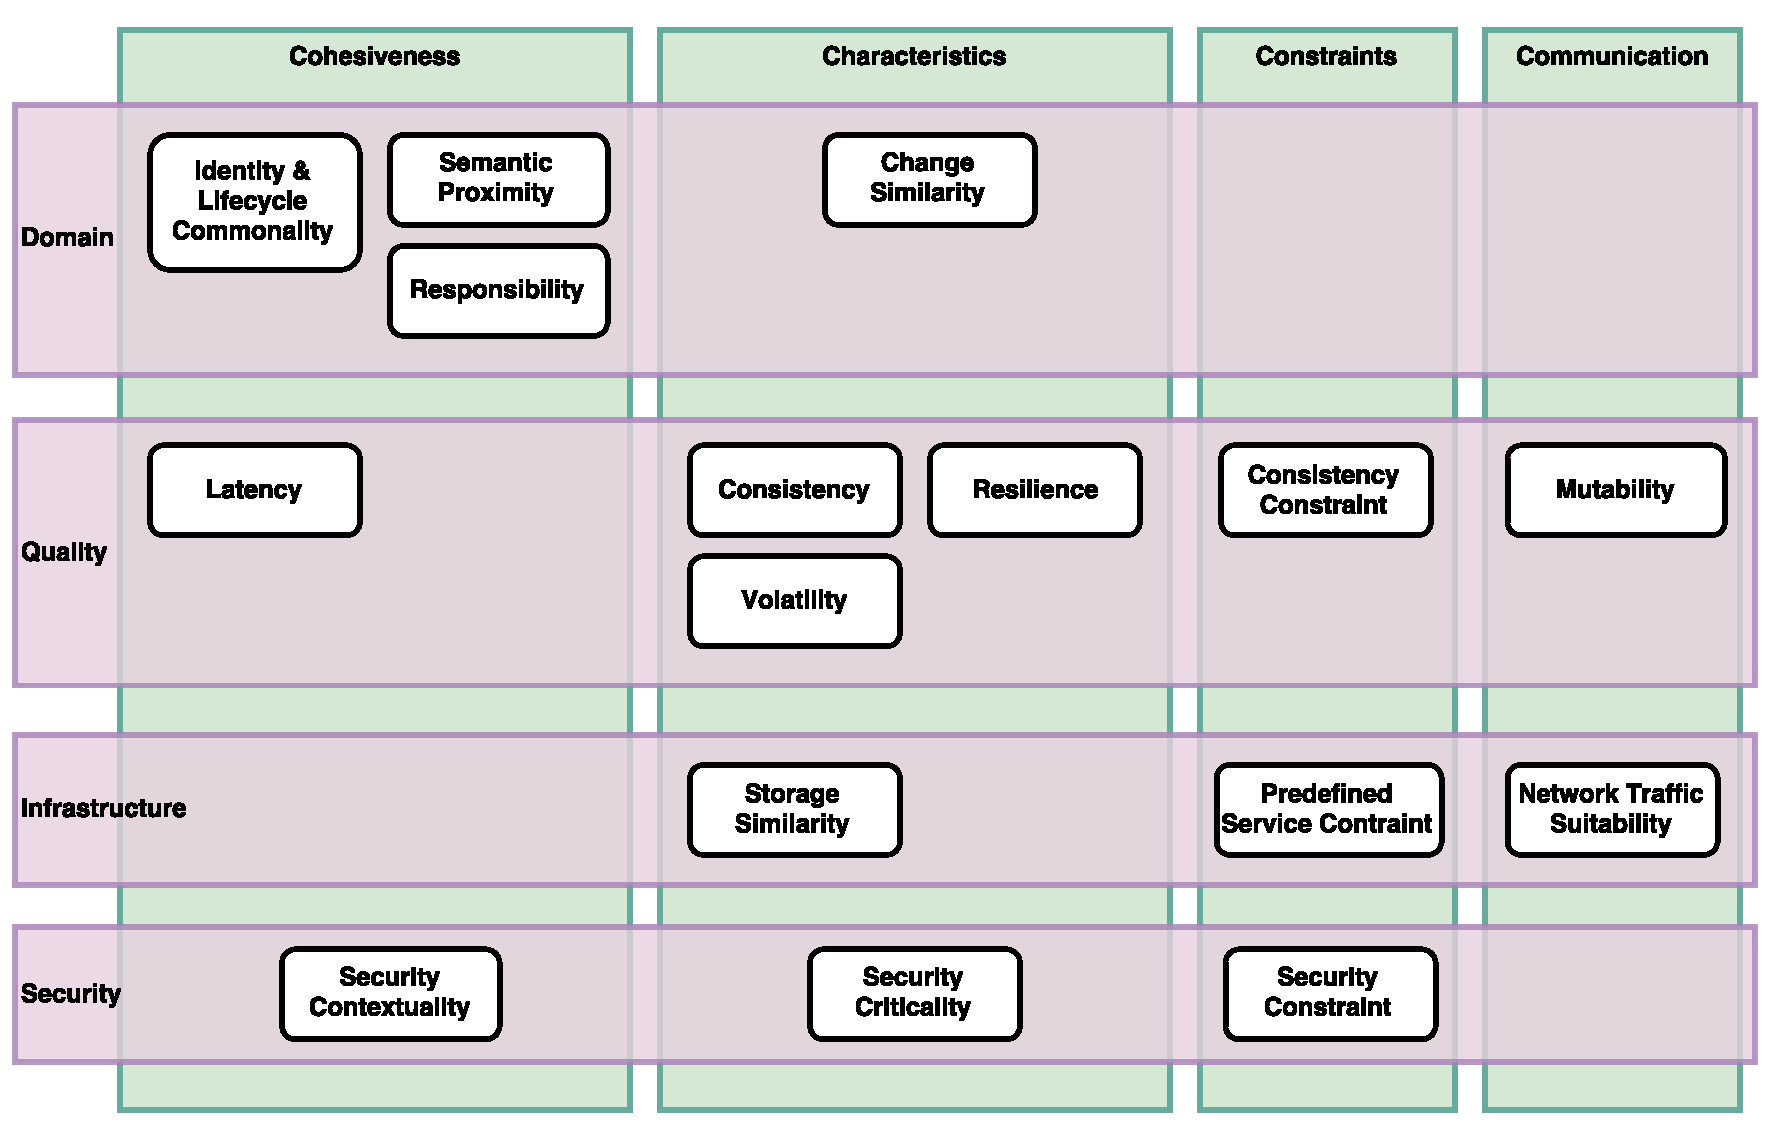
\includegraphics[scale=0.5]{diagrams/CouplingCatalog.pdf}}
	\caption{Coupling Criteria Catalog}
	\label{fig:cc-catalog-mgmt-summary}
\end{figure}


\subsubsection{Service Cutter}

Complementary to the catalog we described an approach to process coupling criteria in a software to optimize loose coupling between services and high cohesion within services. We prototypically implemented the Service Cutter, shown in Figure \ref{fig:ServiceCutter-mgmt-summary}, to verify this approach.

The Service Cutter analyzes a user's \gls{system} based on its nanoentities. Nanoentities are elements used by a service to provide business capabilities. They are defined either as data fields, operations or artifacts. The system is decomposed into services by defining a certain number of services and assigning all nanoentities to exactly one service.

A user can specify his system by means of well established software artifacts such as the entity-relationship model or use cases. Based on these specifications, the coupling between nanoentities is quantified with a score for each coupling criterion. 

\begin{figure}[H]
	\centering{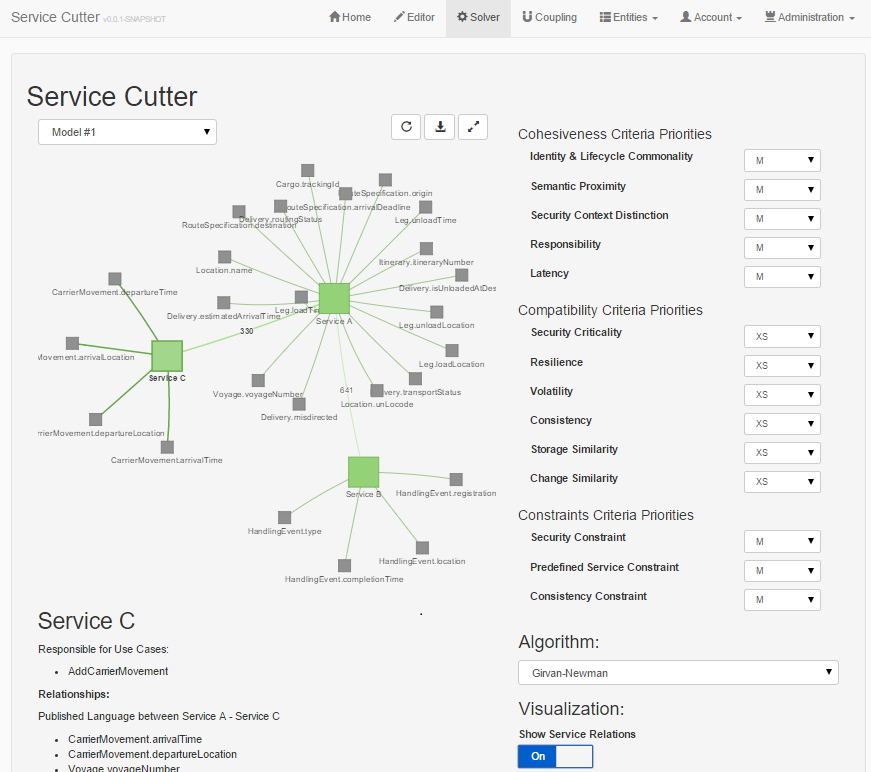
\includegraphics[scale=0.45]{images/ServiceCutter.png}}
	\caption{Screenshot Service Cutter}
	\label{fig:ServiceCutter-mgmt-summary}
\end{figure}

The exact importance of coupling is highly dependent on the context of a software system. Consistency for example is significantly divergent in a banking environment compared to an online social network. To reflect this, we rate the coupling criteria scores using priorities.

\subsubsection{Decomposition by Graph Clustering}

All scores are collected and utilized to construct a weighted, undirected graph. The vertices represent nanoentities and the weighted edges embody the strength of the coupling between two nanoentities.	

Once the graph is constructed, a graph clustering algorithm calculates clusters cutting as few edges as possible. A cluster represents a candidate service. Edges connecting nodes of two clusters represent coupling between the services. This process produces candidate service cuts with high cohesion and low coupling. Figure \ref{fig:mgmt-summary-graph} illustrates a graph created to analyze a sample application.

\begin{minipage}[t]{0.6\textwidth}
	\setlength{\parskip}{5pt plus 0.1pt}
We utilized two complementary graph clustering algorithms. Girvan-Newman takes the desired number of clusters as parameter and is especially suitable for scenarios where a monolithic system is sequentially decomposed into services. The \enquote{Epidemic Label Propagation} algorithm by Leung computes the number of clusters by itself and therefore suggests a suitable number of services to the user. 

We performed tests based on an imaginary \enquote{Trading System}, heavily inspired by real banking software, and the sample application \enquote{Cargo Tracking} as introduced by Eric Evans in his book on Domain Driven Design. The Leung algorithm provided expected or applicable service cuts for both systems while Girvan-Newman only met our expectations for the Trading System. 
\end{minipage}
\begin{minipage}[t]{0.4\textwidth}	
	\begin{figure}[H]
		\begin{center}
			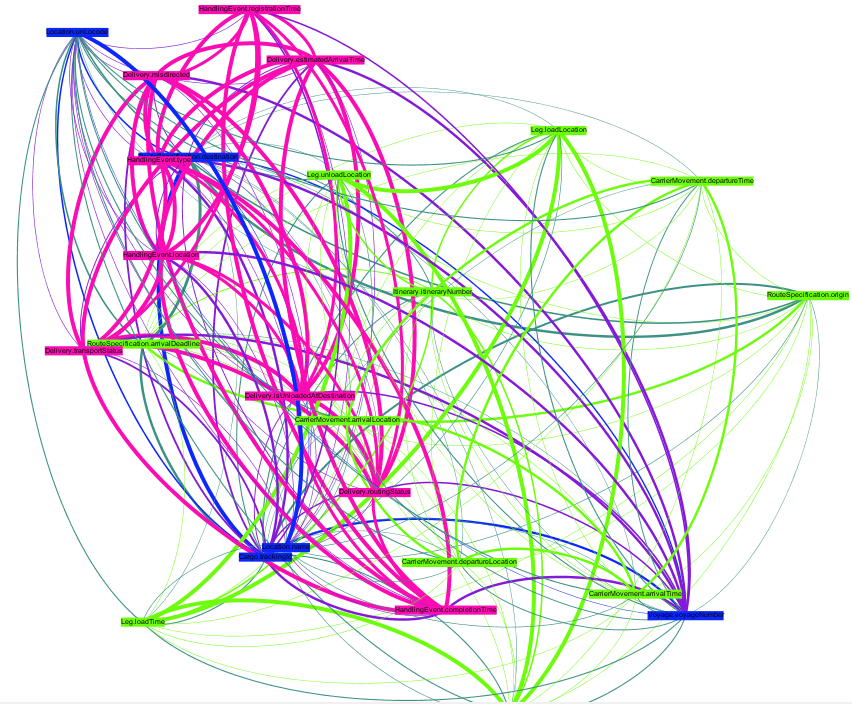
\includegraphics[scale=0.3]{images/ddd_semantic_proximity_debug.png}
			\caption{A graph created for the Cargo Tracking application. The colors represent the detected clusters.}
			\label{fig:mgmt-summary-graph}
		\end{center}
	\end{figure}
\end{minipage}

\subsubsection{Conclusion}
In our thesis, we structured the architecturally significant requirements for service decomposition into the coupling criteria catalog. The test results suggest that these criteria are quantifiable and can be optimized leveraging algorithms and software. 

The Service Cutter structures and assists the decision making process for new or already existing systems. We suggest that future projects either focus on tool development to integrate the Service Cutter into existing software development processes or invest in further research scoring and algorithms. 

\chapter{Introduction}

This chapter introduces the project's goals, scope and context. The original project definition, signed at the beginning of project, is documented in Appendix \ref{appendix:projectDefinition}.

\section{Hypothesis}

D. L. Parnas published a paper titled \textit{On the Criteria To Be Used in Decomposing Systems into Modules}\cite{parnaDecomposing} in 1972. Since then, decomposition of software systems has become an important area in the field of software engineering. As systems grew more complex, software engineers started to distribute modules over computer networks and hence called them services. Architectural styles like Software Oriented Architecture (SOA) have been introduced to tackle many challenges of such distributed systems.

Nevertheless, even with microservices, the latest incarnation of service orientation, decomposition is more described as an art than a structured discipline. C. Richardson writes in his popular introduction to microservices on \gls{infoq}:

\begin{quote}
	\textit{Deciding how to partition a system into a set of services is very much an art but there are number of strategies that can help. One approach is to partition services by verb or use case.}\cite{richardson2014microservices}
\end{quote}

We consider the described strategies as suitable approaches to service decomposition. However, we assume that service decomposition can be approached in more structured way. This leads us to our first hypothesis:

\begin{quote}
	\textit{The driving forces for service decomposition of a software system can be assembled in a comprehensive criteria catalog.}
\end{quote}

To validate this first hypothesis, we created a comprehensive but not conclusive catalog of coupling criteria as a product of the thesis. Taking this structured approach to service decomposition a step further, we formulated a second hypothesis:

\begin{quote}
	\textit{The data of the criteria catalog can be processed in a software to optimize loose coupling between services and high cohesion within services in a structured and automated way.}
\end{quote}

To validate this second hypothesis, we developed a prototype based on the criteria catalog. This tool, hence called the \enquote{Service Cutter}, analyzes a system's specification and suggests candidate service cuts in order to optimize loose coupling between services and high cohesion within services. A system's specification contains an entity-relation model, use cases, and further artifacts as illustrated in Figure \ref{fig:serviceCutterIO}.

\begin{figure}[H]
	\begin{center}
		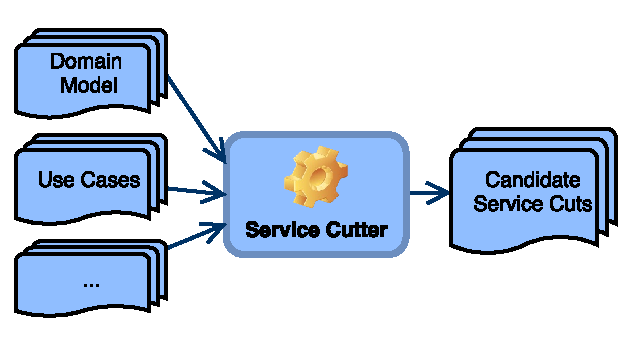
\includegraphics[scale=1.1]{diagrams/systemContextDiagram.pdf}
	\end{center}
	\caption{Input and Output of the Service Cutter}
	\label{fig:serviceCutterIO}
\end{figure}

The Service Cutter's goal is to assist and advise a software architect or developer in his design decisions regarding service decomposition. The architect needs to assess the candidate service cuts and compare them with his expectations. The Service Cutter's mission is accomplished, if the architect's expectations are verified or unexpected but reasonable candidate cuts challenge his preoccupations. 

\section{Project Scope}

This section describes the scope and boundaries of this thesis. 

Throughout the document, a \textit{system} refers to a software application whose architecture needs to be decomposed.

A \textit{service} can be seen as a module providing a remote \gls{API} to communicate with other services. The term is explained in more detail in Chapter \ref{cha:analysis}.

\textit{Service decomposition} refers to splitting a system's functionality and data into services. While we focus on service decomposition, most of the concepts are also true for non-distributed systems where a software internally is decomposed into modules. 

Before a system can be decomposed, its functional and non-functional requirement need be be analyzed and specified in a domain model, use cases, and other artifacts. Based on these specifications the system can be decomposed into services. These are later implemented and connected using intra service communication. Figure \ref{fig:context} illustrates this process.

\begin{figure}[H]
	\begin{center}
		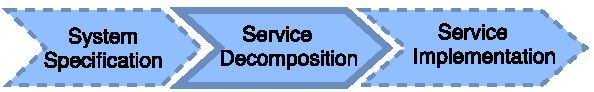
\includegraphics[scale=1.4]{diagrams/context.pdf}
	\end{center}
	\caption{The thesis in the context of system development}
	\label{fig:context}
\end{figure}

Our thesis focuses solely on service decomposition. Consequently the following areas are not in scope:

\begin{itemize}
	\item Requirements engineering and system specification need to be done before a system can be analyzed with the Service Cutter.
	\item Intra service communication is not in scope of this thesis. S. Newman documents in his book \textit{Building Microservices}\cite{newman2015building} multiple popular ways for intra service communication like \gls{RPC}, RESTful HTTP services or asynchronous event-based collaboration. Decomposition only defines \textit{what} is communicated but now \textit{how}. 
	\item Composing multiple services into workflows or business processes using notations like \gls{BPMN} is not in scope.
	\item Service decomposition tries to minimize coupling between services. Tactics like caches or \gls{CQRS}, which try to lower the consequences of coupling introduced by decomposition, are not analyzed. 
\end{itemize}


\section{Context and Influences}

The ideas and concepts in this thesis are influenced by the work of many others. We reused and embodied existing concepts to our structured way of service decomposition. This section describes the context and influences of the thesis.

\subsection{Service Oriented Architecture}

It was during a course titled \textit{Advanced Distributed Systems Design using SOA \& DDD} by Udi Dahan where our initial idea to assist service decomposition with an automated approach emerged. Dahan is the founder of NServiceBus\cite{nservicebus}, the most popular service bus for \gls{dotnet} and a well known \gls{SOA} and \gls{DDD} expert. The approach to tackle service decomposition from the 4+1 View Model\cite{fourPlusOne} is inspired by him. Approaching decomposition on the basis of data fields, or the later in the document introduced nanoentites, is motivated by his course.

Further \gls{SOA} influences are provided by our supervisor throughout the project and during his course \textit{Application Architecture} at \gls{HSR}.

\subsection{Microservices}

In recent years, microservices substituted \gls{SOA} as the trending architectural style, but can be seen as a new incarnation of the service oriented approach. Valuable concepts like service definitions or decomposition criteria are inspired by leading evangelists in this area such as Martin Fowler, Sam Newman, and Chris Richardson. 

\subsection{Domain-Driven Design}

Nevertheless, decomposition is not solely a problem in distributed systems. Eric Evans introduced in his book \textit{Domain-Driven Design: Tackling Complexity in the Heart of Software}\cite{evans2003domain} a collection of patterns to handle decomposition complexity. Especially the concepts \textit{Aggregate}, \textit{Entity}, \textit{Published Language} and \textit{Bounded Context} are integrated in our approach and serve as input or output of the Service Cutter

\section{Existing Decomposition Solutions}

We were not able to find projects that try to structure and automatically assist service decomposition. Nevertheless, there are several methodologies and decomposition tools tackling some of the relevant challenges. 

\subsection{Software Methodologies}

The already introduced approaches \gls{SOA}, microservices, and \gls{DDD} discuss some decomposition criteria but do not provide a comprehensive criteria catalog. 

Other approaches tackle related problems but are focused on different layers of software development. \gls{OOAD} focuses more on abstractions like classes and object instances. We integrated \gls{OOAD} artifacts like the \gls{ERM} as part of the system description given to the Service Cutter as input. \gls{BPM} lays an abstraction layer above services, focusing on business processes and therefore the usage of services rather than their identification and specification. A detailed analysis on the correlation of \gls{OOAD} and \gls{BPM} with service orientation was published by IBM\cite{zimmermann2004elements}. Service oriented modeling approaches like \gls{SOMA}\cite{arsanjani2004service} target similar questions as this thesis but do not provide detailed description of decomposition approaches. \gls{SOMA} suggests decomposition by use cases which resembles our decomposition criterion \textit{Semantic Proximity} introduced in Chapter \ref{cha:decomposition}.

\subsection{Decomposition Tools}

Kenny Bastani suggests a graph based analysis to decompose monolithic software into microservices\cite{bastani}. In his decomposition approach he focuses on dependencies from user stories to resources. He uses Neo4J GraphGist\cite{graphGist} to visualize the dependencies but does not run any automated analysis on the graph. 

The barrio eclipse plugin\cite{dietrich2008cluster} analyzes dependencies based on Java source code. It suggests a candidate package structure by leveraging the Girvan-Newman clustering algorithm. The tool has been published as part of a students project of the Massey University, New Zealand.

\bigskip

After introducing our hypothesis's and the broader context of service decomposition, the next Chapter analyzes the definition of a service and service decomposition principles in more detail. 

%TODO AppArch 3 Ebenen von Services,  Drei definitionen von SOMA/Services, User / Architect / Developer



\chapter{Domain Analysis}
\label{cha:analysis}

This chapter analyzes the concepts of services and service decomposition in more detail and concludes with a questionnaire that helps to assess decompositions. 

\section{Service Definition}
\label{sec:serviceIntro}

\textit{Service} is one of the most used terms in the field of software architecture and has been defined differently in many papers, books, and blog posts in numerous ways and various contexts. This section consolidates multiple definitions and defines service for this thesis.

\subsection{Different Views on Services}

The \enquote{4+1 View Model of Software Architecture} by Philippe Kruchten\cite{fourPlusOne} describes software architecture using the views \textit{Logical View}, \textit{Physical View}, \textit{Development View}, and \textit{Process View} which are illustrated by \textit{Scenarios}. During our research we discovered that the difficulty to clearly define the word service lies in the fact that different definitions focus on contrasting views. For this thesis we use multiple definitions for the term service depending if we write about the \textit{logical} or the \textit{physical} view of a service.

\subsubsection{Logical Service}

\begin{quotation}
\textit{A service is the technical authority for a specific business capability} \newline --- Udi Dahan\cite{serviceDefinitionDahan}
\end{quotation}
   
This definition focuses more on the logical or scenario view of a service than its technical representation. He further defines that all data and operations required to provide a business capability are owned by one and only one service. 

Udi Dahan implies that a service is not restricted to a specific application, process, technology or layer. In fact, it contains required layers itself, including databases, logic, and \gls{UI} code.

A logical service is autonomous and composed from many processes, webservices or databases, but keeps a clear boundary and interface against the outer world. Communication with other parts of the system only happens on a well defined interface on a common communication channel.

\subsubsection{Bounded Context}

Another concept describing logical services is the bounded context as defined in the Domain-Driven Design\cite{evans2014domain}:

\begin{quotation}
	\textit{A description of a boundary (typically a subsystem, or the work of a particular team) within which a particular model is defined and applicable.}
\end{quotation}

A model only used within one bounded context is defined and visible only in that context. Accordingly, a model used in multiple services needs to have a globally shared definition, defined as \textit{Published Language} in the context of \gls{DDD}\cite{evans2014domain}:

\begin{quotation}
	\textit{The translation between the models of two bounded contexts requires a common Language.}
\end{quotation}

The process of service decomposition as done by the Service Cutter automatically defines the published language of the system. 

\subsubsection{Physical Service}

Martin Fowler describes a service as following:

\begin{quotation}
	\textit{A service will be used remotely through some remote interface, either synchronous or asynchronous.}\cite{fowlerIoC}
\end{quotation}

This definition by Martin Fowler is based on the physical structure and is close to what recently has been advertised as a \textit{microservice}:

\begin{quotation}
	\textit{In short, the microservice architectural style is an approach to developing a single application as a suite of small services, each running in its own process and communicating with lightweight mechanisms, often an HTTP resource API.}\cite{fowlerMicroservice}
\end{quotation}

A process providing a remote API might provide business logic, pure technical functionality or a data store. A service commonly includes at least a data store, wrapped by a RESTful HTTP API. Physical services might be congruent with logical services but very often more complex cases split logical services in multiple physical services. 

\subsubsection{Should the Service Cutter Produce Logical or Physical Service Candidates?}

The Service Cutter incorporates logical and physical aspects in the decomposition process but focuses more on the former. 

Not all reasons to create physical services can be analyzed in a structured way. The Service Cutter cannot decide if a service using a database runs in a single process or connects to its database over a remote interface. Similarly, an operations team might decide to run different logical services on the same machine or even in the same process to save resources and simplify deployment. These decisions are often reasoned by operational aspects rather than the system's characteristics. 

Nevertheless, some physical aspects can be analyzed. As an example, the Service Cutter is able to receive information about the storage requirements for the system's data. It suggests that data with very high storage requires an own service because a different database technology is necessary. 

We define that the Service Cutter focuses on logical services while incorporating physical aspects whenever possible. 

\subsection{Nanoentities, Building Blocks for Services}

Sam Newman writes in his book \textit{Building Microservices}\cite[p. 34]{newman2015building}: 

\begin{quote}
	\textit{When you start to think about the bounded contexts that exist in your organization, you should be thinking not in terms of data that is shared, but about the capabilities those contexts provide the rest of the domain.}
\end{quote}

In order to provide capabilities, a service needs resources. We identified three types of resources which are the building blocks of services:

\begin{description}
	\item[Data] A service has ownership over some of the system's data. It is the only instance responsible for changes on that data and optionally informs other services about changes. The data is often, but not necessarily, stored in a database. Data which is published to other services belongs to the published language of the system.
	\item[Operations] A service has ownership over business rules and calculation logic. These operations are often, but not necessarily, based on the data the service owns.
	\item[Artifacts] A service has ownership over artifacts. An artifact is a collection of data or operation results transformed into a specific format. An example is a business report which has been built using operations and data.
\end{description}

In order to enable a structured approach to service decomposition, we generalize these resources with the concept of a \textit{nanoentity}. Examples for possible nanoentities are illustrated in Figure \ref{fig:nanoentities}.

\begin{figure}[H]
	\centering{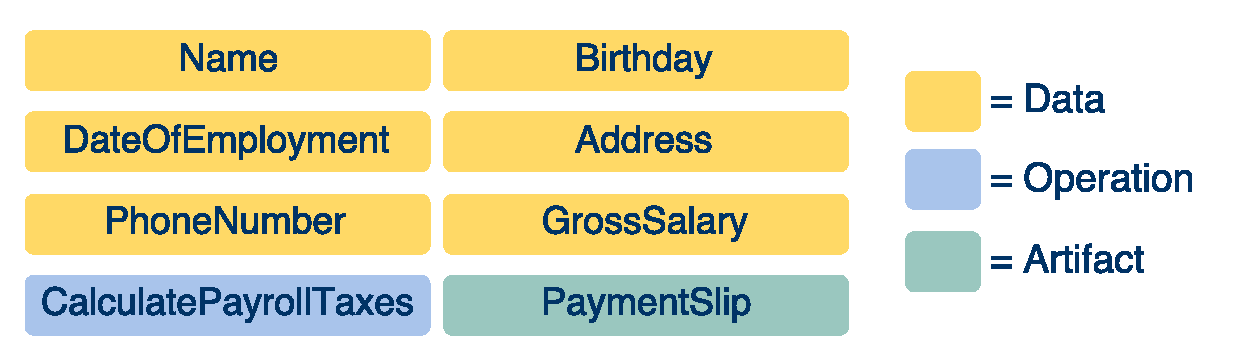
\includegraphics[scale=0.7]{diagrams/Nanoentities.pdf}}
	\caption{Nanoentities related to an employee.}
	\label{fig:nanoentities}
\end{figure}	

A service must contain  at least two type of nanoentities to be considered a logical service. 
\begin{itemize}
\item Something only providing CRUD\footnote{Create, Read, Update, and Delete} functions on data is considered a database. 
\item Something only providing operations is considered a function. 
\item Something only providing artifacts is considered a resource or a database. 
\end{itemize}

Service decomposition is the act of defining a number of services and assigning all nanoentities to the responsible service. The driving forces for decomposition are discussed in more detail in the next section.


\section{Service Decomposition}

Well experienced software architects decompose systems by reason of driving forces to ensure a maintainable, robust and consistent system with business relevance and good performance. This section describes the forces mostly considered by architects. 

Decomposition has been a main discipline for programmers since early in the history of our industry. David L. Parnas published a paper entitled \enquote{On the Criteria To Be Used in Decomposing Systems into Modules} in 1972\cite{parnaDecomposing}. Shortly after, the terms \textit{coupling} and \textit{cohesion} as software design metrics appeared as part of the \textit{Structured Design} technique\cite{structuredDesign}:

\begin{description}
	\item[Coupling] \textit{A measure of how closely connected two routines or modules are.\newline In	software design, a measure of the interdependence among modules in a computer program.}\cite{softwareVocabulary}
	\item[Cohesion] \textit{The manner and degree to which the tasks performed by a single software module are related to one another.} \newline 
	\textit{In software design, a measure of the strength of association of the elements within a module.}\cite{softwareVocabulary}
\end{description}

Software architects commonly started to use these metrics to define that good architectures have high cohesion within and low coupling between its parts. Robert Martin later described a general principle to achieve loose coupling and high cohesion:

\begin{description}
	\item[Single Responsibility Principle] \textit{Gather together the things that change for the same reasons. Separate those things that change for different reasons.}\cite{SRP}
\end{description}

Starting from these principles, we analyzed different types of coupling and cohesion and created the decomposition model described in the next chapter.


\chapter{Decomposition Model}
\label{cha:decomposition}

The decomposition model describes the quality attributes of good service decomposition solutions and the criteria leading to such. This chapter starts with an overview over all defined coupling criteria and concludes with the definition of a good decomposition solution. 

A coupling criterion describes an architecturally significant requirement why two nanoentities should or should not be owned by the same service. These criteria define the semantic model on which the Service Cutter is built on. 

The coupling criteria in this thesis are a product of literature research and a workshop assembling the collective software architect experience of our thesis advisor Prof. Dr. O. Zimmermann, our industry partner represented by W. Giersche, an architect of Zühlke Engineering, and us. We transformed the resulting ideas into the following structured catalog.

\section{Catalog Overview}
\label{subsec:couplingCriteriaOverview}

We arranged the coupling criteria in a grid as shown in Figure \ref{fig:cc_grid}.

The grid columns represent the following partitions:

\begin{description}
	\item[Cohesiveness] - Criteria describing the cohesiveness of nanoentities and therefore why they should belong to the same service. 
	\item[Compatibility] - Criteria describing the divergent characteristics of nanoentities. The service should not contain nanoentities with different characteristics. Examples for incompatible characteristics are \enquote{High}, \enquote{Eventually}, and \enquote{Weak} for the criterion \textit{Consistency Criticality}.
	\item[Constraints] - Criteria describing constraints which enforce that group of nanoentities must be distributed amongst different services or form a service by itself. (No entities are assigned to another service; no entities are added to this service.)
	\item[Communication] - Criteria describing which nanoentities are suitable to be used as part of the published language shared between services. 
\end{description}

\clearpage
The rows are inspired by the \enquote{4+1 View Model of Software Architecture} by Kruchten\cite{fourPlusOne}. Domain is an enhancement of the \textit{Logical View}, quality resembles the \textit{Process View} and physical matches the \textit{Physical View} but also includes predefined service constraints. Security is included in the \textit{Development View} by Kruchten. We decided to promote it to a separate layer as it was a prominent requirement in our workshop and other aspects of the \textit{Development View} were not relevant for our application.

\begin{description}
	\item[Domain] Criteria describing nanoentities from a business domain perspective.
	\item[Quality] Criteria describing the quality requirements of a nanoentity directly or the related use case. Non-functional requirements are predominantly represented in this row.
	\item[Physical] Criteria describing the infrastructural or technological aspects of nanoentities.
	\item[Security] Criteria describing nanoentities from a security perspective.
\end{description}

\begin{figure}[H]
	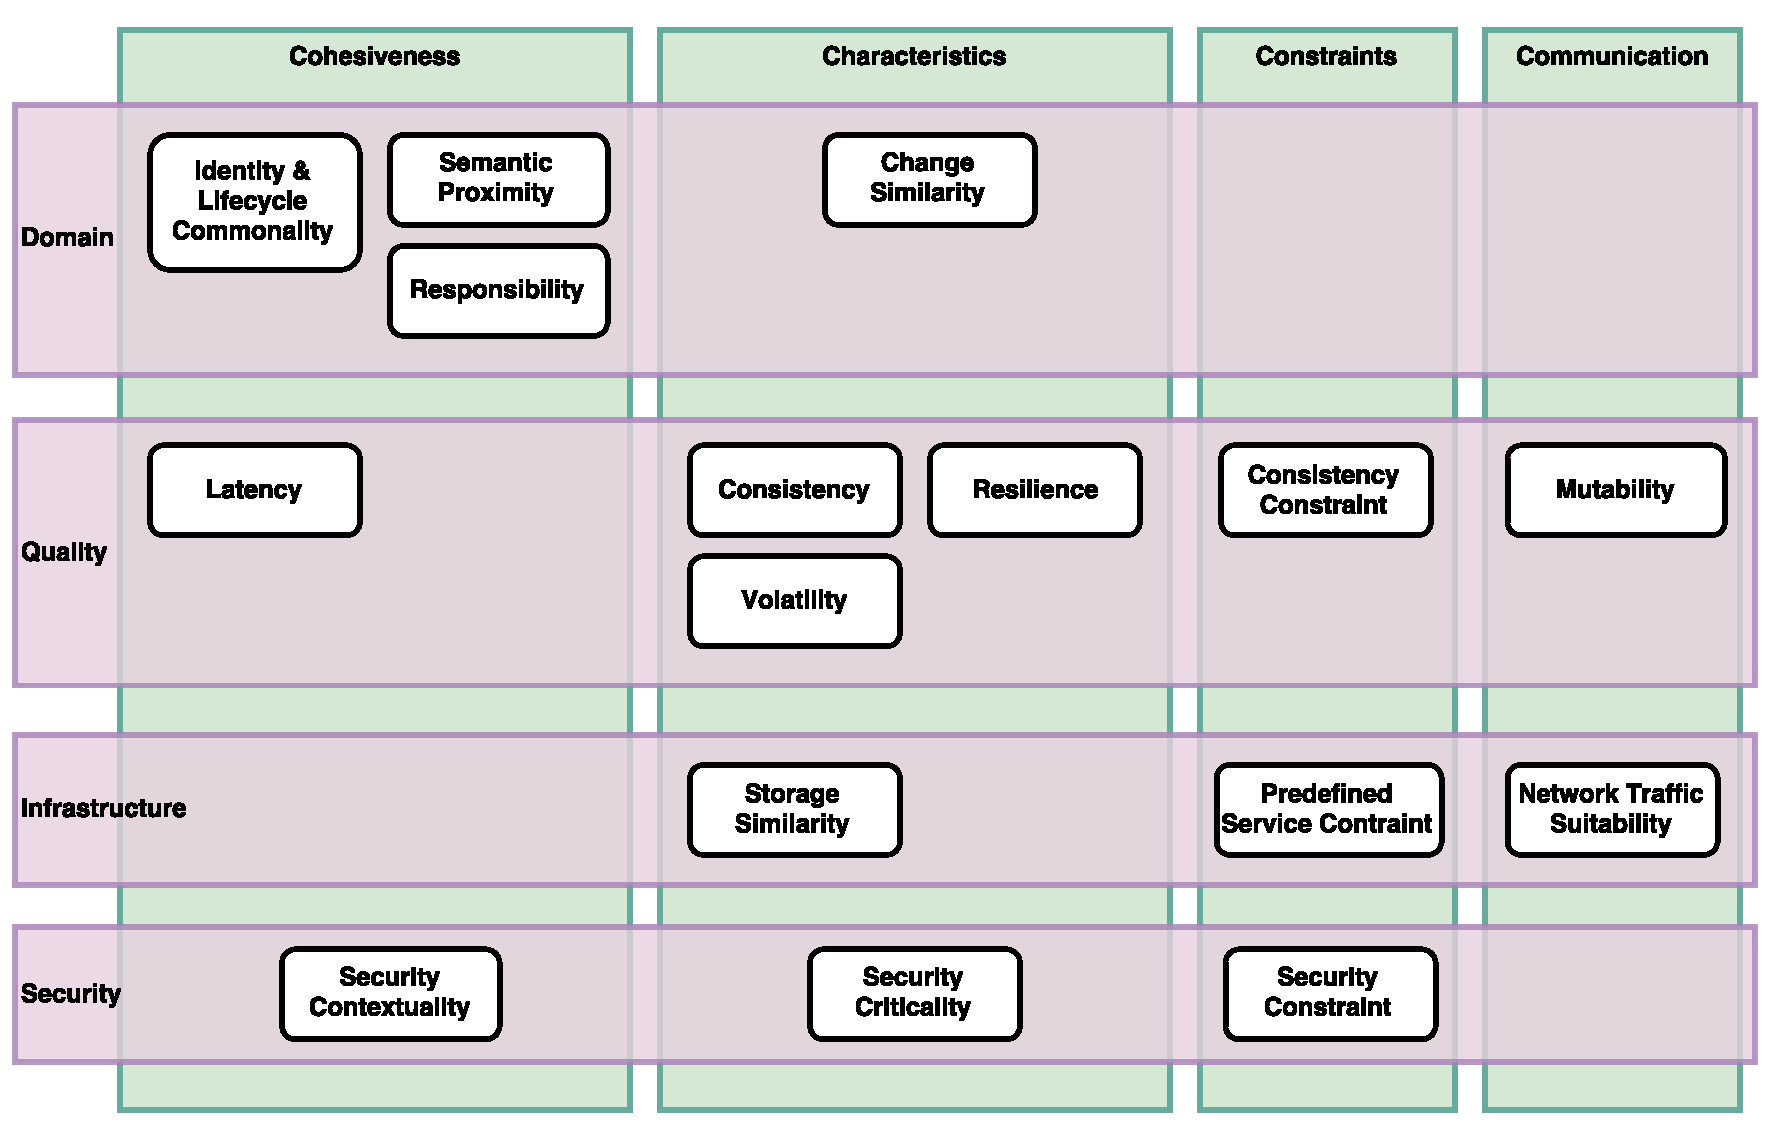
\includegraphics[scale=0.5]{diagrams/CouplingCatalog.pdf}
	\caption{Coupling criteria grid}
	\label{fig:cc_grid}
\end{figure}

\clearpage
\section{Coupling Criteria Cards}
\label{sec:couplingCriteriaCards}

We specified all coupling criteria listed in the grid as \enquote{CC cards} like the following:

\newcommand{\ccCard}[8] {
\begin{minipage}{\linewidth}
	\begin{framed}
	\textbf{#1 #2}
	
		\begin{description}[leftmargin=!,labelwidth=\widthof{\bfseries User Representation}]
		\item[Description] #3
		\item[User Representation] #4 %TODO source?
		\ifthenelse{\equal{#5}{}}{}{\item[Literature] #5}
		\item[Type] #6
		\item[Perspective] #7
		%\ifx #8\empty  #8 \fi
		\item[Characteristics] \ifthenelse{\equal{#8}{}}{n/a}{#8}
		\end{description}
	
	\end{framed}
\end{minipage}
}
\ccCard{CC-1}{Identity \& Lifecycle Commonality}{Nanoentities that belong to the same identity and therefore share a common lifecycle. }{- UML class diagrams (Same Class, Composition, Inheritance) \newline - Domain-Driven Design entities.}{Entity definition in Domain-Driven Design: \newline \textit{Some objects are not defined primarily by their attributes. They represent a thread of identity that	runs through time and often across distinct representations.}\cite{evans2003domain}}{Cohesiveness}{Domain}{}


Cards share the following information:

\begin{description}
	\item[Description] Explains the coupling criteria in more detail.
	\item[User Representation] Lists concepts familiar to the architect that can be used to feed the criteria information into the Service Cutter.
	\item[Literature] References the coupling criteria to descriptions in existing literature.
	\item[Type] The type of the criterion: Cohesiveness, Compatibility, Constraint or Communication.
	\item[Perspective] The perspective of the criterion: Domain, Quality, Infrastructure or Security. 
	\item[Characteristics] Cards of type \enquote{compatibility} list different characteristics that can be applied to a nanoentity.
\end{description}

\ccCard{CC-2}{Semantic Proximity}{Two nanoentities are semantically proximate when they have a semantic connection given by the business domain. The strongest indicator for semantic proximity is coherent access on nanoentities within the same use case.}{- Coherent access or updates on nanoentities in use cases.\newline - Aggregation or association relationships in UML class diagrams.}{C. Richardson on microservice decomposition:\newline \textit{Deciding how to partition a system into a set of services is very much an art but there are number of strategies that can help. One approach is to partition services by verb or use case.}\cite{microserviceIntro}\newline Single Responsibility Principle by R.~C.~Martin:\newline \textit{Gather together the things that change for the same reasons. Separate those things that change for different reasons.}\cite{SRP}}{Cohesiveness}{Domain}{}
%todo literature based on use case driven services?

\ccCard{CC-3}{Shared Owner}{The same person, role or department is responsible for a group of nanoentities. Service decomposition should try to keep entities with the same responsible role together while not mixing entities with different responsible instances in one service. }{User defined persons, roles or departments with each containing a group of nanoentities. A nanoentity can only be associated once.}{Conway's law:\newline \textit{Organizations which design systems are constrained to produce designs which are copies of the communication structures of these organizations.}\cite{conway}\newline Single Responsibility Principle by C. Martin:\newline \textit{Gather together the things that change for the same reasons. Separate those things that change for different reasons. [...] However, as you think about this principle, remember that the reasons for change are people. It is people who request changes. And you don't want to confuse those people, or yourself, by mixing together the code that many different people care about for different reasons.}\cite{SRP}}{Cohesiveness}{Domain}{}

\ccCard{CC-4}{Structural Volatility}{How often change requests need to be implemented affecting nanoentities.}{Classification of nanoentities in characteristics.}{D.~L.~Parnas on modular programming: \newline \textit{We propose instead that one begins with a list of difficult design decisions or design decisions which are likely to change. Each module is then designed to hide such a decision from the others.}\cite{parnaDecomposing}}{Compatibility}{Domain}{Often, Normal \textit{(default)}, Rarely}

Structural Volatility refers to the frequency of changes to the logic or data structure (\gls{DDL}) and requires a redeployment. Updates on the data itself is reflected in the coupling criterion Content Volatility (\gls{DML}).

\ccCard{CC-5}{Latency}{Groups of nanoentities with high performance requirements for a specific user request. These nanoentities should be modelled in the same service to avoid remote calls.}{Use cases with latency requirements. All nanoentities read or written by the same use case belong a group. A nanoentity can belong to multiple groups.}{Design guidelines for application performance by Microsoft: \newline \textit{Minimize round trips to reduce call latency. For example, batch calls together and design coarse-grained services that allow you to perform a single logical operation by using a single round trip.}\cite{performance}}{Cohesiveness}{Quality}{}

\ccCard{CC-6}{Consistency Criticality}{Some data such as financial records loses its value in case of inconsistencies while other data is more tolerant to inconsistencies.}{Classification of nanoentities in characteristics.}{W. Vogel on consistency requirements: \newline  
\textit{\textbf{Strong consistency}: After the update completes, any subsequent access (by A, B, or C) will return the updated value. \newline \textbf{Weak consistency}: The system does not guarantee that subsequent accesses will return the updated value. A number of conditions need to be met before the value will be returned. The period between the update and the moment when it is guaranteed that any observer will always see the updated value is dubbed the inconsistency window.}\cite{consistency}}{Compatibility}{Quality}{High consistency \textit{(default)}, eventual consistency, weak consistency}

\ccCard{CC-7}{Availability Criticality}{Nanoentities have varying availability constraints. Some are critical while others can be unavailable for some time. As providing high availability comes at a cost, nanoentities classified with different characteristics should not be composed in the same service.}{Classification of nanoentities in characteristics.}{E. Woods on availability and resilience: \newline \textit{Getting your availability characteristics wrong can be very expensive. However, increased online availability comes at a cost, whether in terms of more hardware, increased software sophistication, or redundancy in your communications network.}\cite{rozanski2011software} }{Compatibility}{Quality}{Critical, Normal \textit{(default)}, Low}

\ccCard{CC-8}{Content Volatility}{A nanoentity can be classified by its volatility which defines how frequent it is updated. Highly volatile and more stable nanoentities should be composed in different services.}{- Volatility can be calculated from use case definitions if they are equipped with a frequency information. \newline- Nanoentities can be classified by data types to determine the volatility: Master Data (regularly), Reference Data (rarely), Transaction Data (often) and Inventory Data (often) to determine the volatility.}{}{Compatibility}{Quality}{Often, Regularly \textit{(default)}, Rarely}
%TODO add literature (datentypen?)

%TODO data:  DDL, artifact: report regenerated

\ccCard{CC-9}{Consistency Constraint}{A group of nanoentities that have a dependent state and therefore need to be kept consistent to each other. }{An aggregate as defined in domain-driven design.}{Aggregate as defined in domain-driven design by E. Evans: \newline \textit{A cluster of associated objects that are treated as a unit for the purpose of data changes. External references are restricted to one member of the aggregate, designated as the root. A set of consistency rules applies within the aggregate's boundaries.}\cite{evans2003domain} \newline U.~Dahan on service decomposition: \newline \textit{If modifying the value of one attribute involves changing the value of another, then those two attributes should fall under the responsibility of the same service.}\cite{udiConsistency}}{Constraint}{Quality}{}

A \textit{Consistency Contraint} differs from the \textit{Consistency Criticality} coupling criteria in such a way that the constraint groups a set of nanoentities ensuring their atomic processing. 

For example a payment and the account balance should be linked using a \textit{Consistency Constraint}. The Service Cutter therefore guarantees that those fields are in the same service. The \textit{Consistency Criticality} criterion is of type compatibility and only separates divergent characteristics.

\ccCard{CC-10}{Mutability}{Immutable information is much simpler to manage in a distributed system than mutable objects. Immutable nanoentities are therefore good candidates for the published language shared between two services. Service decomposition should be done in a way that favors sharing immutable nanoentities over mutable ones. }{Classification of each nanoentity in mutable or immutable.}{U.~Dahan on finding service boundaries:\newline \textit{When you find something immutable, that is an indication that there is some loose coupling between the two sides passing immutable data.}\cite{mutability}}{Communication}{Quality}{}

Developing nanoservices in an immutable manner is an implementation style that simplifies distributed communication and is not always possible to achieve. Volatility in contrast is an attribute whose characteristics can be assigned to all nanoservices. %TODO lukas: review!

\ccCard{CC-11}{Storage Similarity}{Storage that is required to persist all instances of a nanoentity.}{The user classifies nanoentities into the given characteristics. The classification is system specific. In one system a nanoentity classified as \textit{huge} might need 1MB, but in another 1GB storage per instance.}{}{Compatibility}{Infrastructure}{Huge, Normal \textit{(default)}, Tiny}

\ccCard{CC-12}{Predefined Service Constraint}{There might be the following reasons why some nanoentities forcefully need to be modelled in the same service: \newline - Technological optimizations \newline - Legacy systems}{User defined service with each containing a group of nanoentities. Each nanoentity can be associated only once.}{}{Constraint}{Infrastructure}{}

\ccCard{CC-13}{Network Traffic Similarity}{Service decomposition has a significant impact on network traffic, depending on which nanoentities are shared between services and how often. Small and less frequently accessed nanoentities are better suited to be shared between services.}{Use cases define the frequency of access on nanoentities. The size of each entity can be determined by CC-11: Storage Similarty}{}{Communication}{Infrastructure}{}

\ccCard{CC-14}{Security Contextuality}{A security role is allowed to see or process a group of nanoentities. Mixing security contexts in one service complicates authentication and authorization implementations.}{User defined security roles with each containing a group of nanoentities. A nanoentity can be associated to multiple groups.}{}{Cohesiveness}{Security}{}

\ccCard{CC-15}{Security Criticality}{Criticality of an nanoentity in case of data loss or a privacy violation. Represents the reputational or financial damage when the information is disclosed to unauthorized parties. As high security criticality comes at a cost, nanoentities classified with different characteristics should not be composed in the same service. }{Classification of nanoentities in characteristics}{}{Compatibility}{Security}{Critical, Internal \textit{(default)}, Public}

\ccCard{CC-16}{Security Constraint}{Groups of nanoentities are semantically related but must not reside in the same service in order to satisfy information security requirements. This restriction can be established by an external party such as a certification authority or an internal design team.}{Demilitarized zones or other groups of nanoentities that should be composed to different services.}{}{Constraint}{Security}{}



% \ccCard{CC-}{}{}{}{}{}{}


\section{What is a good Decomposition Solution?}
\label{sec:decompositionRequirements}

The following questionnaire is based on the coupling criteria described in this chapter and aims to fulfill the principles introduced in Chapter \ref{cha:analysis}. In a good decomposition solution, the answer to all those questions should be \enquote{yes}.

\begin{enumerate} %TODO is it possible to remove some of the negation?
	\item Does it not violate a constraint criterion?
	\item Does it not combine too many nanoentities with diverging characteristics into one service?
	\item Does each service depend on as few nanoentities of other services as possible? A use case should cross as few service boundaries as possible. %Do a small amount of use cases require more than one service to be completed?
	\item Are the nanoentities that are part of a published language between services suitable for intra service communication?
	\item Is the coupling between services similar? It is not the size of services that requires homogeneity within the system but the amount of published language the services. 
	\item Are there not too many services? This is called the nanoservice antipattern\cite{nanoservice}.
	\item Are there not too few services? This is a monolithic architecture.
\end{enumerate}

Those questions could form a check-list to validate a service cut suggested by the Service Cutter. This approach is outlined in Section \ref{sec:suggested-cut-grades}.


%TODO User stories as most important criteria: check Ivar Jacobson, oose, a use case driven approach

%TODO: Should we describe non relevant coupling criteria as well? (Hiding design decisions etc, see CC catalog doc)

%TODO: (Bring result \& discussion already here?)



\chapter{Requirements}
\label{cha:requirements}

%TODO: describe the service cutter as a solution finding tool (not a architecture builder) either here or in introduction

This chapter describes the (non-)functional requirements of the target solution and covers the characteristics of it's target users. 

The requirements in this chapter are not prioritized. As part of the sprint planning meetings, these requirements are transformed to tasks and prioritized. The description in this chapter is meant to provide a high level overview and establish a common sense between all stakeholders of this project.


\section{Personas}

Our personas are based on ??. % TODO workshops, interviews, discussions?

All users of the system are experienced software architects or developers interested in the educational aspects of the tool.


%TODO other persona Ideas: High level architect, developr and Business analysts

\subsection{Junior Jedi-Master}

Junior has been a fast growing and aspiring developer since he graduated from university with a master's degree in information technology eight years ago. In his new job, Junior finds himself in the role of an architect for a new and promising product that enjoys the support of well known investors. In consequence of his experience in distributed systems, he has been assigned with the task to decompose the system's business model into logical services of which each will be split into multiple separately deployable microservices. 

Junior strongly believes in automation and using every tool available to support and complete his work. For his current project he plans to try the Service Cutter as a foundation and verification of his architectural decisions. 


\subsection{Walter Wisenheimer}

Walter is an architect with many years of experience in the industry and has built numerous systems already. Walter has seen many automation concepts and tools failing their goals. In Walter's view a natural and obvious outcome -- an architect's world is too complex to model and automate in a system or algorithm. 

After a longer discussion with an over-motivated greenhorn who recently joined his company, Walter starts to see the benefits of the well structured format the Service Cutter organizes architecturally relevant information. Using the tool to structure and document his systems characteristics might be of some benefit as currently most of this information is only known to himself. 

Walter decided to try the Service Cutter to structure the information for the current project he is working on.

%\subsection{Charles Consultant}

%TODO necessary?

\subsection{Stan Student}

Stan studies Computer Science and as part of his class in Service oriented Software Architecture he is supposed to design a set of services for the ZooKeeper domain. The Service Cutter guides him through the important decisions by asking a set of questions and presents him a set of possible service cuts. 

Being overwhelmed of all the data requested by the Service Cutter he would like to configure the tool to only focus on the data he got provided in his exercises. 

Stan then discusses the advantages and disadvantages of the presented options with his fellow students. He furthermore asks his Professor about the to him unknown criteria the Service Cutter requested and why that information might have an impact on service orientation. 


\subsection{Tom Tutor}

Tom wants to introduce his students to the software architecture craft. He uses the Service Cutter to visualize the different ways of distribute data into services during his lectures. By changing the calculation parameters he can demonstrate that software architecture mostly depends on the context of the requirement. The same problem might have different solutions in varying circumstances.


\section{Functional Requirements}

The Service Cutter faces the functional requirements presented in the following
section.

%TODO machen wir user stories?

%TODO: each data field needs a master who is the only one doing writes.

%TODO low prio: Add relations between coupling criteria. examples: High volatility and high security is dangerous. Or high criticality and high change management. The Service Cutter could generate warnings if theses things are put together in the same service or either consider theses r


%TODO low prio: Show warnings as part of the output should a predefined service have a significant negative effect!

\subsection{Data Fields and Entities}

A set of data fields can either be defined in the application or imported using a predefined data format. A data field consists of it's name and a combination of connections to other fields, referred to as Coupling Criteria.

The process of putting fields in relation to each other should use as many familiar concepts as possible. The concept of an entity - a set of fields sharing a commdon identity and lifecycle\cite[p.13]{evans2014domain} - is a widely used notion and is therefore used by the architect to model the data and then mapped to the Coupling Criteria \enquote{Shares Lifecycle} and \enquote{Common Identity} by the system.

\subsection{Coupling Criteria}

Almost all data fields are related to other fields. The concept of a Coupling Criterion is used to characterise such connections.

A list of relevant Coupling Criteria was identified in a workshop with Zühlke. The following Criteria are supported by the system:

\begin{itemize}
	\item Shares Lifecycle
	\item Common Identity
	\item Inheritance
	\item Volatility
	\item Security
	\item Resilience
	\item Use Case
\end{itemize}

%TODO liste ergänzen nach workshop!

\subsection{Service Boundaries}

Once the user has added all data fields and coupling criteria he can calculate the suggested service boundaries. An algorithm groups fields in a way that minimizes coupling between the groups while maximizing the cohesion inside a group.

The calculation can be parametrised using weights assigned to coupling criteria. In this way different service boundaries can be calculated for different requirements. For example in an application that processed financial data, security might be more important than Use Cases. In a different context, e.g. for an application that needs to support high volumes of data, volatility and resilience might be a primary focus.

\subsection{Service Coupling}

Some Coupling Criteria will likely span across service boundaries. The architect uses the graphical representation of the Service Cutter to inspect the coupling. Using this information he might change the calculation parameters to achieve a different service cut.

Service Coupling maps to the Published Language as described by Evans \cite[p.375]{evans2003domain}.

% link zu published language von DDD?

% TODO:  Quantification is configurable – but the system provides a good default
\section{Nonfunctional Requirements}
\label{sec:nonfunctionalRequirements}

The following non-functional requirements should be satisfied by the Service Cutter.

\subsection{Usability}
\label{sec:usability}

A software architect should be able to use the software without any training. All controls are clearly named and, where appropriate, documented using an inline user manual including representative samples.

The user gets well introduced to the important concepts of the Service Cutter. These concepts include:

\begin{enumerate}
	\item A Service and service decomposition
	\item A system's model (nanoentities)
	\item Coupling criteria, their meaning and decomposition impact
	\item User representations and their impact on coupling criteria
	\item Characteristics values, coupling criteria priorities and final ratings.
\end{enumerate}

Often used configuration like coupling criteria priorities should be shown directly to the user to encourage its usage. More advanced configuration like the weights of coupling criteria variants should be accessible for the user but do not need to be shown directly in a standard workflow. 

Up to 2000 nanoentities and 200 entities need to be manageable without losing track.

\subsection{Simplicity}

A simple system analysis can be achieved with not more than 5 clicks. All steps are provided with useful defaults that can be changed.

\subsection{Performance}

All regular user interactions should not take more than one second.

Calculations of service cuts should meet the following conditions assuming a data set of 100 entities and 2000 nanoentities.

\begin{itemize}
\item Calculations that are used once per day should take less than 10 minutes.
\item Calculations that are used once per minute should take less than 5 seconds.
\end{itemize}

\subsection{Monitoring, Logging, Deployment, Availability}

The scope of this thesis is to prototypically implement the Service Cutter. Operational aspects only need to be covered on a basic level:

\begin{itemize}
	\item Log files should be written using SLF4J\cite{slf4j}.
	\item Deployment should be provided with Docker\cite{docker} containers.
\end{itemize} 

\subsection{Fault Tolerance}

As the prototype does not need to handle ever possible use case or unexpected input, a common error handling needs to be built into the application and ensures that operations continue even in case of unexpected input or state.

\subsection{Maintainability}

In case of a success the prototype might be the basis for further development or other thesis projects. It should be built in clearly separated modules (or even remote services) to ensure good maintainability. At least the following modules need to be clearly separated:

%TODO thesis plural

\begin{enumerate}
	\item Internal representation of coupling criteria
	\item Data of a users system (nanoentities, use case definition etc.) 
	\item Decomposition algorithm (Solver)
	\item User interface
\end{enumerate}

If one or multiple of the modules are implemented as physical services the remote \gls{API} needs to be implemented as RESTful HTTP interface. 

The application should leverage existing open source frameworks or libraries wherever possible to ensure a minimal maintenance effort.

\subsection{State-of-the-Art Technology}

To support further development of the Service Cutter the prototype needs to be implemented in state-of-the-art technology. Our industry partner Z\"uhlke has suggested the following technology stack:

\begin{enumerate}
	\item Java Spring\cite{spring} as a base framework. 
	\item JHipster\cite{jhipster} with Spring Boot\cite{springboot} for project setup.
	\item AngularJS\cite{angularjs} and Bootstrap\cite{bootstrap} for the user interface.
	\item Docker\cite{docker} for container and deployment configuration and handling. 
\end{enumerate}

\subsection{License}

All involved parties decided to release the Service Cutter under the terms of the Apache 2.0 open source license.


\bigskip

After defining all (non-)functional requirements, the next Chapter outlines design and implementation steps which were taken to satisfy these requirements.




\chapter{Design and Implementation}
\label{cha:implementation}

\section{Decomposition Algorithm}

Decomposition describes the task of grouping data fields into services. Achieving a good solution according to the defined Coupling Criteria as described in \ref{sec:decompositionRequirements} requires a non trivial algorithm. This section documents the evaluation process for such an algorithm.

\subsection{Approach \#1: Clustering of a Weighted Undirected Graph}
\label{subsec:approach1_graph}

Our first approach to solve the decomposition problem was using a weighted, undirected graph with a clustering or community algorithm. 

Every data field in the model is represented by a node. Edges define a relationship between two data fields. The weight on each edge shows how \textit{close} or \textit{cohesive} two fields are. The higher the weight, the more likely they should belong to the same service. Figure \ref{fig:weighted_graph} shows an abstract example of such a graph.

\begin{minipage}[t]{0.5\textwidth}
	Figure \ref{fig:graph_approach} outlines a solution sketch for this approach. As user representations are imported, data fields and  information for predefined Coupling Criteria are extracted by the \textit{Importer} to store all important information to create the graph.
	
	The \textit{Solver} then creates all vertices from the data fields and builds edges between them according to the stored Coupling Criteria instances. This task contains complexity for the following reasons:
	
	\begin{enumerate}
		\item Coupling Criteria are not homogeneous as described in Section \ref{subsec:couplingCriteriaTypes}. 
		%TODO: write first about types before completing this item. Mention distance, closeness and cumulative criteria
		
		\item All Coupling Criteria information is reduced to a single number with one single unit of measurement. An increase of the weight for one Criteria automatically changes the relative importance of that CC to others.
		
		\item To give the user a way to define the specific requirements of his system, priorities per Coupling Criteria can optionally be defined to influence the weights of each Coupling Criteria instance. 
	\end{enumerate}
	
	The \textit{Clustering Algorithm} then analyzes the graph and creates clusters of data fields so that as few edges as possible need to be cut.
	
	\begin{figure}[H]
		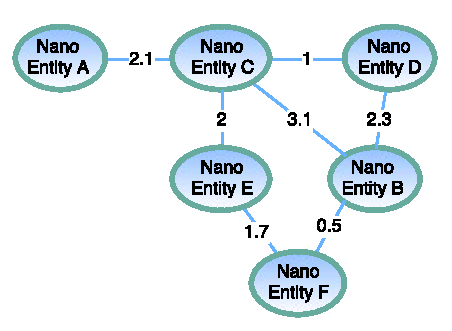
\includegraphics[scale=1.0]{diagrams/weighted_graph.pdf}
		\caption{Example of a Weighted Graph}
		\label{fig:weighted_graph}
	\end{figure}

\end{minipage}
\begin{minipage}[t]{0.5\textwidth}
	\begin{figure}[H]
		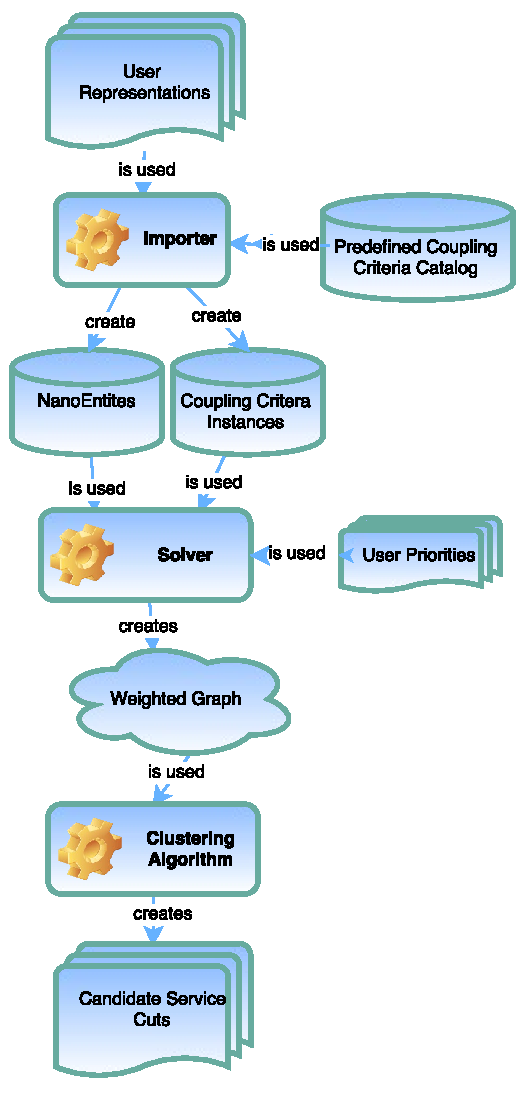
\includegraphics[scale=1.0]{diagrams/graph_approach.pdf}
		\caption{Solution Sketch for a Weighted Graph with a Clustering Algorithm}
		\label{fig:graph_approach}
	\end{figure}
\end{minipage}

A detailed evaluation of clustering algorithms is document in Appendix \ref{appendix:graphClustering}. We decided to do a first assessment of this approach with the MCL\cite{mcl} and Girvan-Newman\cite{girvanNewman} algorithms. Both algorithms are implemented as plugins of the Gephi\cite{gephi} platform and can be extracted as \gls{JAR} files.

\subsubsection{Practical Assessment of the Graph Clustering Approach}

To assess the graph approach we use a simple booking domain model. In Figure \ref{fig:clusteringBookingSimple} the MCL algorithm was run on the booking model with all Coupling Criteria priorities set to zero expect the Variant \textit{Same Entity} of the \textit{Identity \& Lifecycle Commonality} Criteria. Consequently the visualized Services contain one entity each. The entities can be identified as \textit{Customer}, \textit{Article} and \textit{Customer}.

\begin{figure}[H]
	\begin{center}
		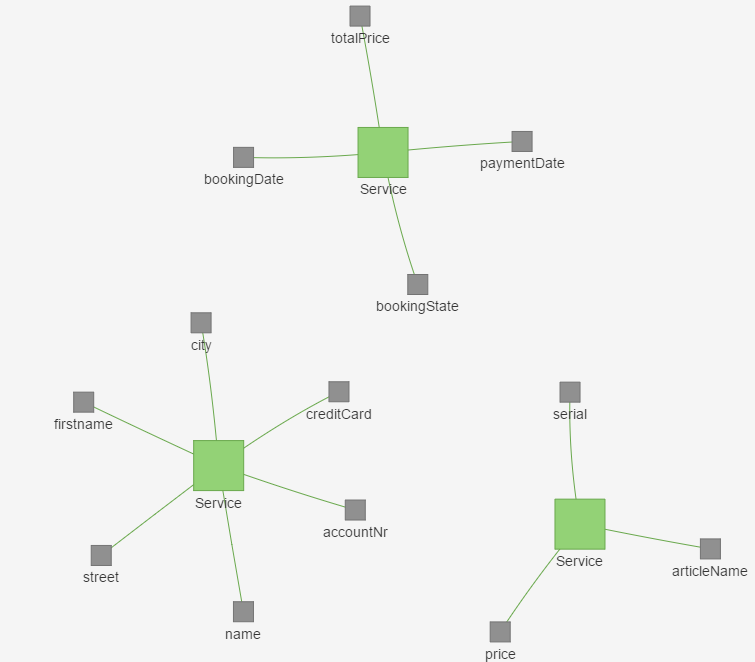
\includegraphics[scale=0.8]{images/booking_entities.png}
	\end{center}
	\caption{Clustering of a simple Booking example.}
	\label{fig:clusteringBookingSimple}
\end{figure}


Figure \ref{fig:clusteringBooking} shows the result of the MCL algorithm with user stories of the Booking domain added. 

\begin{figure}[H]
	\begin{center}
		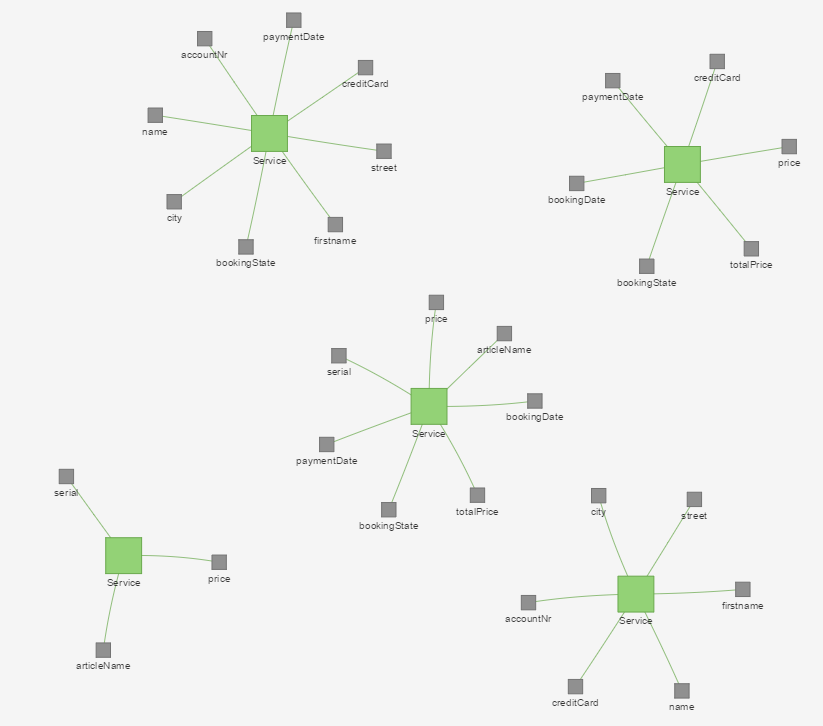
\includegraphics[scale=0.7]{images/booking_entities_mcl.png}
	\end{center}
	\caption{Booking Example enhanced with User Stories.}
	\label{fig:clusteringBooking}
\end{figure}

Obviously this is not the result expected. The requirement that a data field should be once and only once grouped to a Service is not met and the meaning of each Service can't be interpreted. 


\subsubsection{Theoretical Assessment of the Graph Clustering Approach}
Theoretical assessment


\subsection{Approach \#2: Set Rating}

\subsection{Approach \#3: Constructing Services - a Heuristic Approach}

\section{Prototype} 

\subsection{Design}

\subsection{Technology}

\subsection{Infrastructure}

\subsection{Information Security}

The web application is secured using an authentication and authorization implementation. Any other internal components such as the database or web services are hidden behind the servers firewall and therefore do not need any special security measures.

The uploaded data models are initially shared amongst all registered users.

\subsection{User Interface}

The base layout is responsive and adapts to smaller screens such as smartphones. However the tool is mostly used on devices such as laptops and the controls are therefore optimized for use on screens that are at least 15 inches wide and used with a mouse and a keyboard.


\bigskip
After covering the important design and implementation aspects, the next chapter assesses the built solution described in this chapter against the defined requirements.


\chapter{Working with the Service Cutter} 

%TODO Potential contents of this chapter:
\begin{itemize}
	\item How do you organize such an interview?
	\item Documentation of input format?
	\item When to choose which algorithm?
	\item Recommendations for working with the priorities.
\end{itemize}

This section outlines our proposed usage schemes.

%TODO: Does this chapter make sense? it could cover the process of working with the service cutter, finding the needed information, intepreting the results and using it for decision finding and documentations (ADs). Giersche highly recommended/requested this. 
\subsection{Data Population}

\begin{enumerate}
	\item UML Class Diagram
	\item Use Cases or User Stories
	\item Contextual information
\end{enumerate}

How do you initially populate all the coupling data? LOTS of knowledge is required!

Hard to keep it up to date.

\subsection{Usage Scenarios}

- from monolith to microservices
- green field services, replicable priorities

\subsection{Interpreting the Result}

?
\subsection{Development Iterations}

What to do with the output? How to feed it back into the loop in the next release cycle?


After introducing usage scenarios of the service cutter, the next chapter assesses the decomposition approach and the practicability of the Service Cutter

\chapter{Discussion}

This chapter discusses the outcome of the thesis, the Service Cutter and its impact for future work.


%TODO Broader algorithm testing. Also non-Java implementations

\section{Thesis Evaluation}

At the beginning of this project we formulated two hypothesizes. We were able to produce results proving both of them.
%TODO convert goals to reference?

%Die Gründe für Service Cuts in einem Softwaresystem kann man als Liste von \enquote{Coupling Criteria} umfassend beschreiben.
\begin{quote}
	\textit{The driving factors for service cuts in a software system can be compiled into a comprehensive criteria catalog.}
\end{quote}

We successfully compiled a catalog of 14 coupling criteria that aims to form a comprehensive but not conclusive collection. 

The catalog helps a software architect to structurize driving factors for service decomposition while providing a good system documentation. The developed criteria may provide a basis for a common language amongst architects. 

%Ziel erreicht. umfassend - aber nicht abschliessend. der katalog kann aus unserer sicht einen diskussionsbeitrag liefern und zum beispiel eine grundlage für eine gemeinsame sprache für architekten liefern.

\begin{quote}
	\textit{The data of the criteria catalog can be embodied in software in order to optimzie loose coupling between and high cohesion within services in a strcutured and automated way.}
\end{quote}
%Die Informationen aus den \enquote{Coupling Criteria} können strukturiert verarbeitet werden, um die Entkopplung von Softwarekomponenten zu optimieren.}

In the Service Cutter assessment documented in Appendix \ref{appendix:serviceCutterAssessment}, we tested two sample systems each with the algorithms Girvan-Newman and Leung. Girvan-Newman provided expected and therefore satisfying results in only one of the two example systems. Leung on the other hand did not only provide expected service cuts for both systems but surprised us with suggestions that were unexpected but definitely reasonable.  


The Service Cutter as of now does not yet provide significant business value to its users. It is not a production grade architectural tool but a proof that our concept of structured and automated decomposition optimization generally works and is worth further investigations. We believe that the great value to its users will become apparent when further efforts are put in the following four aspects:

\begin{enumerate}
	\item The \textbf{scoring process} for the different type of criteria should further be analyzed and tested. More sophisticated solutions for conceptual challenges like the single dimensionality problem documented in Section \ref{subsec:singleDimensionality} could improve the accuracy and meaningfulness of results. 
	\item \textbf{Graph clustering algorithms} should further be analyzed and optimized. Possible alternative approaches as documented in Appendix \ref{appendix:decompositionAppraoches} could furthermore solve some of the conceptual challenges of the scoring process.
	\item The \textbf{Service Cutter Prototype} should be enhanced to a production ready tool with graphical user interfaces for defining, editing, and storing a user's system description and candidate service cuts. %TODO storing user representations?
	\item The idea of the Service Cutter should be integrated into a \textbf{toolkit chain}. The input could automatically be generated from other tools or diagrams and the output used for code or \gls{API} generation.
\end{enumerate}

These aspects are documented in more detail in Chapter \ref{cha:futureWork}.

\section{Requirements Assessment}

This section assesses the developed solution based on the defined requirements. The two domain models as described in Appendix \ref{appendix:serviceCutterAssessment} as well as the implemented Service Cutter itself serve as the test scenario.

All requirements are rated with a rating from $1-3$.

\begin{description}
\item[1] The requirement is fully satisfied.
\item[2] The requirement is partially satisfied.
\item[3] The requirement is not satisfied.
\end{description}

\subsection{Functional Requirements}

Table \ref{tab:conclusionFunctional} assesses the provided solution against the defined functional requirements described in Section \ref{sec:functionalRequirements}.

\begin{table}[H]
	\centering
	\caption{Assessment of functional requirements}
	\label{tab:conclusionFunctional}
	\begin{tabular}{|p{100pt}|l|p{250pt}|}
	\hline \textbf{Requirement} & \textbf{Rating} & \textbf{Assessment} \\ 
	\hline Coupling Criteria & 1 & All coupling criteria have been implemented in the Service Cutter.  \\ %TODO stimmt das wirklich? noch nicht!
	\hline User Representations & 1 & All required user representations are supported by the importer of the Service Cutter. \\ 
	\hline Priorities & 1 & Priorities are built into the scoring process. \\ 
	\hline Candidate Service Cuts & 2 & The Service Cutter visualizes a candidate service cut using a chart. Multiple candidate cuts can only be compared using several browser tabs. \\ 
	\hline Published Language & 1 & The published language is extracted from the candidate service cut when selecting a service node in the visualization.  \\ 
	\hline Hard Architectural Decisions & 2 & This feature is not explicitly implemented but partially given by non-deterministic algorithms as discussed in Section \ref{subsec:algoDiscussion}\\
	\hline 
	\end{tabular} 
\end{table}

\subsection{Non-Functional Requirements}

Table \ref{tab:conclusionNonFunctional} assesses the provided solution against the defined non-functional requirements described in Chapter \ref{cha:requirements}, Section \ref{sec:nonfunctionalRequirements}. %TODO überall so? chapter X, section Y

\begin{table}[H]
	\centering
	\caption{Assessment of non-functional requirements}
	\label{tab:conclusionNonFunctional}
	\begin{tabular}{|p{100pt}|l|p{250pt}|}
	\hline \textbf{Requirement} & \textbf{Rating} & \textbf{Assessment} \\ 
	\hline Usability & 2 & TODO: document in detail \\ %TODO document
	\hline Simplicity & 1 & A simple analysis can be performed with 5 mouse clicks. \\
	\hline Performance & 2 & The sample domain models can be decomposed in not more than two seconds. Extensive performance tests have not been conducted due to time budget constraints as decided with our stakeholders. \\
	\hline Logging, \newline Deployment & 1 & Logging is based on SLF4J and a deployment based on Docker is implemented. \\
	\hline Fault Tolerance & 1 & All errors are handled and occuring errors are logged. \\
	\hline Maintainability & 1 & The implementation is based on two services (editor and engine) both built with suitable application layers. Communication between the layers is implemented with RESTful HTTP communication. Open source tools are used wherever possible. \\
	\hline State-of-the-Art Technology & 1 & The application is based on the technology stack suggested by our industry partner. \\
	\hline License & 1 & The source code has been released under the Apache 2.0 license. \\
	\hline 
	\end{tabular} 
\end{table}


\section{Conclusion}

??
%TODO




\chapter{Future Work}
\label{cha:futureWork}

This chapter explains possible enhancements of the Service Cutter and the coupling criteria catalog. %TODO check, catalog auch?

\section{Scoring}

The developed scoring process works well for our test scenarios. However other systems might require further enhancements.

\subsection{Better Handling for Separations}
\label{sec:handling-for-separations}

As introduced as \textit{single dimensionality} in Section \ref{subsec:singleDimensionality}, we mapped coupling of type compatibility and constraints to negative scores. Once all coupling criteria have been processed, we remove all edges with a negative total score. This approach retains information about the coupling in a system. Finding a solution for the single dimensionality problem would lead to more accurate candidate service cuts.

\subsection{Implement Criteria of Type Communication}

As part of this project we only implemented 14 out of 16 identified coupling criteria. The following two criteria are solely described as part of the decomposition model in Chapter \ref{cha:decomposition}.

\begin{itemize}
\item \textit{Mutability} defined whether a nanoentity is mutable or immutable.
\item \textit{Network Traffic Suitability} illustrates the network traffic implications when this nanoentity is exposed to a remote interface.
\end{itemize}

Both criteria of type \textit{communication} do not describe which nanoentities should or should not be modeled in the same service, but which nanoentities are more suitable for being exposed as published language and therefore used in intra service communication. For immutable data, consistency is not an issue and it is therefore simpler to handle and more suitable for published language then mutable nanoentities. Similarly, nanoentities that are frequently accessed and need high storage resources are less suitable for being exposed on the network. 

If a nanoentity needs to be exposed is defined by use cases and which service is responsible for which use case. The communication criteria require that the use case accessing unsuitable nanoentities are owned by the same services as the nanoentities.

%%% verstehe ich nicht
%Both criteria influence the cost of a service cut. Services owning immutable data with little network traffic can easily be extracted into a separated service. Mutable data causing lots of traffic however should preferrably not be extracted. The scoring concept could be enhanced to also be capable of supporting communication requirements.

\section{Algorithms \& Approach}

This section illustrates a series of possible improvements to the algorithms.

\subsection{Additional Leung Layer}

The non-deterministic nature of the Leung algorithm causes the calculation result to be unstable. This has advantages and disadvantages as outlined in Section \ref{subsec:algoDiscussion}. As an architect, I would expect the Service Cutter to assist me with non-deterministic algorithms in a way that the possible service cuts are automatically calculated, compared and rated. This additional layer would allow me to select the best candidate service cut and help furthermore help to identify hard architectural decisions.

\subsection{MCL adapter}
\label{subsec:mclAdapter}

As outlined in Section \ref{sec:algorithms}, the MCL algorithm could be used in the Service Cutter as well.

The reference implementation of the MCL algorithm is provided as a \gls{c} based command line tool. With some effort this algorithm could be integrated into the Service Cutter using \gls{JNI} or an integration based on text files.

An assessment of the MCL algorithm may produce better results compared to the other algorithms.

\subsection{Alternative Algorithms and Optimizations of Existing Algorithms}

Our evaluation of suitable graph clustering algorithms was limited to the ones having a stable Java implementation. Further research may prove that other algorithms are capable of calculating even candidate service cuts better according to the defined criteria\ref{sec:decompositionRequirements}.

Furthermore existing algorithms may be improved with optimizations. For instance Lancichinetti and Fortunato\cite{lancichinetti2009community} valuated a set of improved versions of the Girvan-Newman algorithm as well as a collection of alternative algorithms.

We assume that optimizations of the Service Cutter's algorithm can be achieved when the selection is not limited to existing Java implementations.

\section{Tooling}

A set of enhancements of the Service Cutter as a tool may increase its value to the users.

\subsection{Traceability of User Representations}

It is important that the calculated data is presented to the user in a way for him to understand why the candidate service cuts have been selected. By visualizing the user's input on candidate service cuts, the user gets a better understanding of how his input and definitions affect the suggested decomposition. 

Along with the user representations, the scores could be visualized per coupling criterion so that the user understands the impact of priority changes and input enhancements. However, this feature should be disabled for a novice user. 

\subsection{Adjust Suggested Solutions}

The architect is able to adjust the solution by moving a nanoentity from one to another service. He instantly sees the impact of his adjustment as the rating of each coupling criterion is visualized.

\subsection{Configurations for Advanced Users}

For a normal usage, the Service Cutter provides reasonable defaults which have been tested with example systems. Advanced users should be enabled to change or enhance existing characteristics of compatibility criteria.

\subsection{Configuration through a Questionnaire}

The Service Cutter could guide the architect through a questionnaire in order to apply different presets of characterization defaults or priorities.

\subsection{Editor for User Representations}

To improve usability and reduce the effort needed to define the input for the Service Cutter, a sophisticated user interface to create and edit user representations should be built. The user interface should simplify input creation as much as possible. One example to achieve this is to the ability to define characteristics on entities which are then applied to all nanoentities of the entity. 

\subsection{Iterative Enhancements}
%TODO: Lukas: Ich verstehe nicht wie das dann funktionieren soll? Sollen wir das nicht umschreiben sodass man models und candidate service cuts einfach persistieren kann?
Projects are often implemented in subsequent stages. The selected service cut of the first iteration influences the design decision of the second iteration. The Service Cutter therefore should allow the user to load a previously persisted service cut into the new model.

\section{Toolchain Integration}

Providing interfaces to existing tools lowers the cost of using the Service Cutter considerably. We therefore recommend to develop integrations with popular software development tools.

\subsection{Adapters for the Input Format}

Writing the required input is a significant effort. The model containing nanoentities and their relations could automatically be parsed from different sources. Adapters could be written for an \gls{ORM} configuration, a database schema, or \gls{UML} diagrams provided by tools like the Enterprise Architect\cite{entArch}.

%TOOD: wie soll das gehen?
%Use cases could be parsed from existing \gls{API} documentation.

\subsection{Use Solution as a Basis for Working Software}

As the Service Cutter has sophisticated information about the usage of nanoentities in use cases, it is able to generate the APIs used to communicate between services. 

Depending on the communication layer used to communicate between services, these \gls{API}s look differently. In a messaging based system the Service Cutter could generate a set of messages or events needed to communicate between services. When services interact by RESTful HTTP interfaces, the Service Cutter is able to generate Swagger\cite{swagger} \gls{API} definitions for the resources which need to be part of the published language of the system. 

\section{Conceptual Refinements}

Besides the technical enhancements, we also collected a set of conceptual improvements.

\subsection{Logical and Physical Services}

As outlined in Section \ref{sec:serviceIntro}, services can be analyzed from different views like the logical or physical view. Udi Dahan describes the confusion of these views as one of the common pitfalls in implementing \gls{SOA}\cite{udiViews}.

In Section\ref{subsec:couplingCriteriaOverview} we categorized the coupling criteria into the views \textit{Domain}, \textit{Quality}, \textit{Physical}, and \textit{Security}. These views should be further analyzed and integrated in the Service Cutter to improve an architect's understanding of different views on his system and the definition of a service. For example, service decomposition could start with candidate bounded contexts by only considering domain criteria. These bounded contexts would further be split into services to when taking the other views into consideration.

%TODO: wie soll das gehen?
%As outlined in Section \ref{sec:serviceIntro} there are two different definitions for the term service. A technical service may contain a number of logical services. This mitigates the cost associated with remoting when two related nanoservices are split into two different services. The Service Cutter could reflect those differences in the scoring logic.

\subsection{Caching}

Caching is data redundancy that is used to reduce the cost of coupling between services. By the means of use cases, the Service Cutter has knowledge of which nanoentities need to be shared between services and, if the use case contains frequency information, even how often it needs to be shared. The Service Cutter could therefore suggest to the architect where caches would be appropriate.

\subsection{Document Architectural Decisions}

\begin{quote}
	Architectural decisions capture key design issues and the rationale behind chosen solutions.\cite{zioAD}
\end{quote}

Documenting architectural decisions is a significant documentation artifact of every long-term software project. In order to retrace architectural decisions taken with help of the Service Cutter, important solutions enhanced with discussion notes could be saved persistently. These notes could be captures as free text, Y-Templates\cite{zimmermann2012yTemplate} or other architectural decision templates\footnote{O. Zimmermann \textit{et al} compiled a comparison of seven publicly available decision templates\cite[p. 3]{zimmermann2015architectural}}.

\subsection{Relationships between Coupling Criteria}

A relationship between coupling criteria like the following might have significant impact on service decomposition:

\textit{Persisted nanoentities with huge storage requirements should not be placed in the same service as nanoentities with high consistency requirements as they are handled using different database technologies.}

Such a relationship should be incorporated in the Service Cutter's decomposition algorithm. Another way of integration would be to present a warning to the user whenever a critical combination of characteristics appears in a candidate service cut.

\section{Candidate Service Cut Grading}
\label{sec:suggested-cut-grades}

We suggested a questionnaire to assess candidate service cuts in Section \ref{sec:decompositionRequirements}. This distinction could automatically be performed by the Service Cutter and visualized using a indicator similar to a traffic light.

%\section{Handling of Large Data Volumes}
%NOTE Lukas: Ist alles bereits abgedeckt in vorherigen Sections

%Our two test systems are relatively small compared to a typical enterprise system. Therefore the required information to analyze such a system is very large. The data model is probably already existing in a machine-readable format -- the use cases however might not exist and a systematic characterization of the nanoentities are likely not available. It is therefore an important question how such a system could be analyzed using the Service Cutter.

%The following questions need to be investigated:

%\begin{enumerate}
%\item Can an existing data model automatically be transformed into the Service Cutter's import format?
%\item Can the Service Cutter calculate meaningful candidate service cuts without taking use cases into account?
%\item Can the Service Cutter offer a \gls{UI} that simplifies characterizations of a large data models?
%\end{enumerate}

%One approach we suggest is to allow a user to specify the coupling on the level of an entity instead of a nanoentity. Other ideas would have to be gathered and evaluated in subsequent projects.



%%%----------------------------------------------------------
%%%Anhang
\appendix



\chapter{Parking Lot}
document not so important findings here	

* Resilience not only per Field definition but also per Instance definition 

* Find Aggregates from Consistency data? Aggregates should not be split between services.

* Decomposition mode: logical or phyiscal. Or: Microservice vs. Module?

* Idea: Only suggested logical services (similarity), then zoom in to see technical services (distance). Algorithm could be splitted into two parts?



\chapter{Decomposition Approach Evaluation}
\label{appendix:decompositionAppraoches}

During early feasibility tests with graph clustering, we encountered significant problems as documented in the next section. As consequence of these results, we conducted a feasibility assessment with a professor of mathematics on the graph based approach, documented in Appendix \ref{sec:feasibilityAssessment}. Out of the feasibility assessment, two additional approaches on how the Service Cutter can solve the decomposition problem were defined and are discussed in this chapter. Nevertheless, the conclusion section states how challenges in these approaches and further research on clustering graphs led us back to follow the graph based approach.

\section{Graph Clustering Problems}

At first, the clustering algorithm evaluated documented in Appendix \ref{appendix:graphClustering} did not contain the Leung algorithm as this has been found later during the project. The two candidate algorithms were MCL and Girvan-Newman. We did a feasibility test using a small booking sample containing three entities:

\begin{description}
	\item[Customer Entity] containing address, accountNr, creditCardNr, and name.
	\item[Article Entity] containing articleName, price, and serial.
	\item[Booking Entity] containing totalPrice, paymentDate, bookingDate, and bookingState.
\end{description}

\begin{figure}[H]
	\begin{center}
		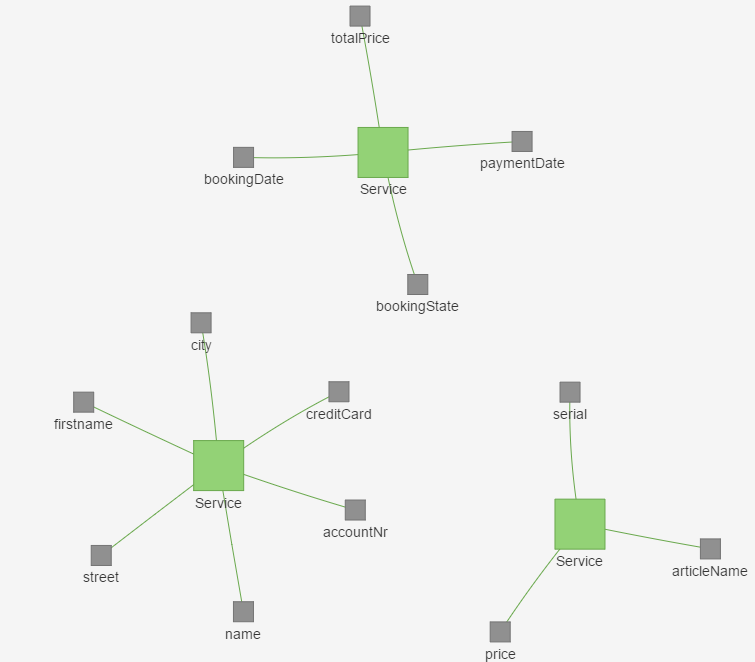
\includegraphics[scale=0.75]{images/booking_entities.png}
	\end{center}
	\caption{Expected output for the booking example}
	\label{fig:bookingExample}
\end{figure}

To keep the sample simple we only added information for the \textit{Lifecycle \& Identity Commonality} criterion, so that the output is expected to show exactly the entity borders as shown in Figure \ref{fig:bookingExample}.


\begin{figure}[H]
	\begin{center}
		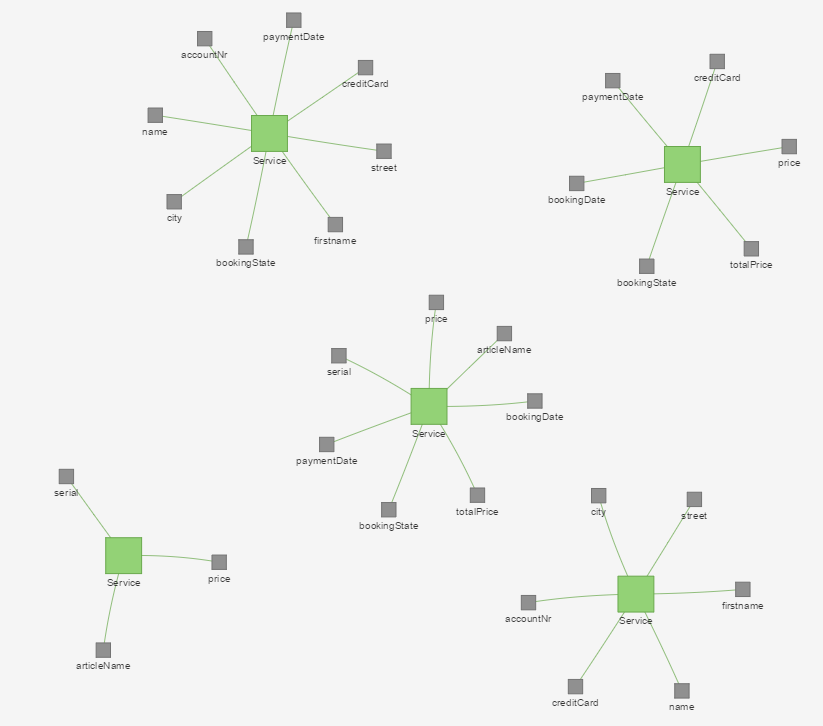
\includegraphics[scale=0.7]{images/booking_entities_mcl.png}
	\end{center}
	\caption{booking sample with the MCL algorithm}
	\label{fig:bookingExampleMCL}
\end{figure}

The MCL algorithm's result for this example is shown in Figure \ref{fig:bookingExampleMCL}. This does not match the expectations as nanoentities are attached to multiple services. This violates the \textit{distinct clusters} requirement. A nanoentity should be assigned to one and only one service. 

The distinct clusters requirement is satisfied by the original MCL algorithm written in C. We therefore assume that this is  an implementation problem of the Gephi plugin\cite{gephiMarkov}. A solution to this problem would be to write a Java wrapper for the C implementation as described in Section \ref{subsec:mclAdapter}.

\begin{figure}[H]
	\begin{center}
		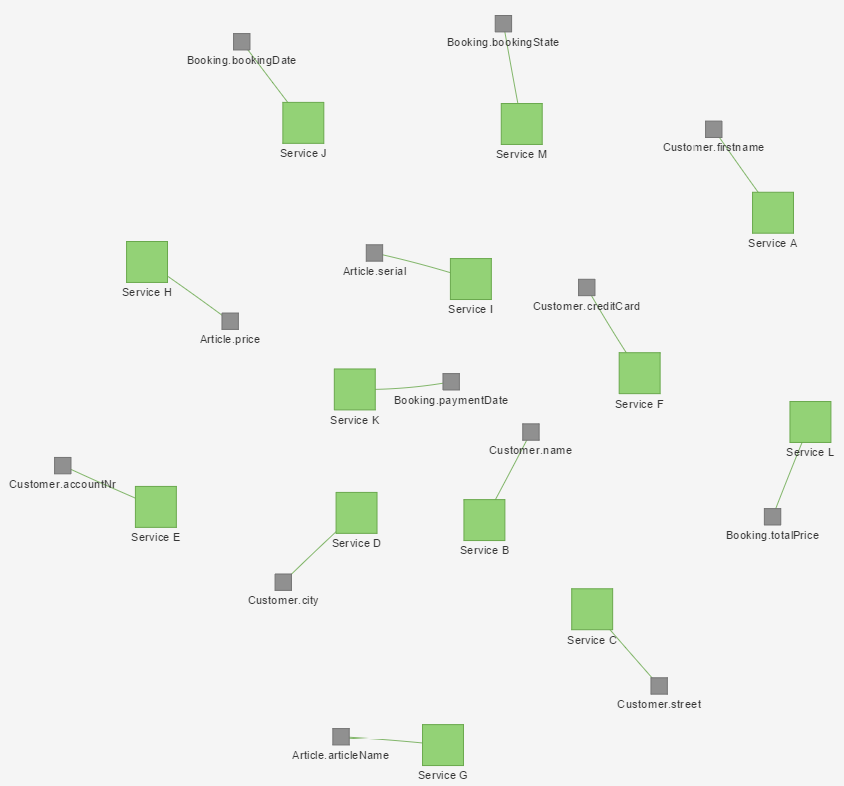
\includegraphics[scale=0.65]{images/girvan_entities_fail.png}
	\end{center}
	\caption{Booking example with the Girvan-Newman algorithm}
	\label{fig:bookingExampleGirvan}
\end{figure}

Figure \ref{fig:bookingExampleGirvan} shows the unsatisfying result provided by Girvan-Newman. By reasons of these unexpected results, we consulted a professor of mathematics as documented in Appendix \ref{sec:feasibilityAssessment} which lead to the alternative approaches described in the next Sections.

\section{Approach \#2: Rating of Possible Service Cuts}

The idea this approach introduces is to create a set of all possible service cuts and rate the cuts isolated per coupling criteria. The approach is illustrated in Figure \ref{fig:setProcess}.

%TODO update Data Fields to NanoEntities, Processor to Scorer
\begin{figure}[H]
	\begin{center}
		\includegraphics[scale=0.45]{diagrams/scoring_process.png}
	\end{center}
	\caption{Approach \#2: Set rating}
	\label{fig:setProcess}
\end{figure}

This approach is processed in three steps:

\begin{description}
	\item[Partitioning] Based on the nanoentities, a set of all possible candidate service cuts is calculated. This includes every theoretically possible service cut for any number of services. For practical usage, this step needs to be optimized. 
	\item[Assessment] For all coupling criteria a processor assesses all service cuts with a score describing how well the criteria's requirements are met. The score is a number between 0 and 10, while 10 implies that all requirements are perfectly satisfied. 
	\item[Evaluation] The user optionally defines priorities how important each criteria is for his system. The priorities are defined with approximately exponential numbers like the Fibonacci sequence. These priorities are applied on the service cut scores. The resulting best candidate cut is then presented to the user.
\end{description}

\subsection{Discussion}

An advantage of this approach is that each relevant step is clearly separated and can thus be analyzed, debugged and visualized better than in the graph based approach. The assessment and score calculation is done separately for every cut and for every coupling criteria. Each criteria scorer scores candidate cuts with a uniform scoring range. As candidate service cuts do not need to be constructed but only rated, the single dimensionality problem described in Section \ref{subsec:singleDimensionality} does not apply.

The weak spot is the partitioning process. Theoretically every possible set of services where each nanoentity is contained in one and only one service is a candidate cut. In mathematics this is described as the \textit{partition of a set}\cite{partitionOfASet} problem. The Bell number $B_n$ defines the amount of possible partitions: 


\begin{displaymath}
B_{n+1}=\sum_{j=0}^n {n\choose j} B_j
\end{displaymath}

For the Service Cutter, $n$ is the number of nanoentities. The number of possible service cuts for $n=20$ nanoentities is $51'724'158'235'372$\footnote{We do not print the number for the required $2000$ nanoentities for lack of space in this document.}.

The Bell number includes cuts for $1 - n$ number of services. In the context of a software system only certain numbers of services are realistic. The \textit{Stirling numbers of the second kind} calculate the Bell number for a given number of sets $k$:

\begin{displaymath}
\left\{ {n \atop k}\right\} = \frac{1}{k!}\sum_{j=0}^{k} (-1)^{k-j} \binom{k}{j} j^n
\end{displaymath}

For $n=20$ nanoentities and $k=4$ services the equation results in $45'232'115'901$ possible cuts. For $k=6$ the result is $4'306'078'895'384$.

During a discussion with our industry partner and supervisor documented in Appendix \ref{sec:status22102015}, we decided that the Service Cutter should be able to process system models with up to 2000 nanoentities. We therefore concluded in the same meeting that this approach is not attainable without a heuristic attempt of finding a small set of relevant candidate cuts. 

A possible heuristic approach is to take into account one or a few coupling criteria information about the system to find service candidates. A simple example would be to only analyze cuts where nanoentities of the same entity are not split across services so that only entities and not its nanoentities need to be considered.

As we tried to find a heuristic approach to calculate candidate cuts, we discovered a new idea for the composition algorithm described in the next section. 

\section{Approach \#3: Constructing Services - a Heuristic Approach}

While analyzing the decomposition problem we realized that finding a good number of services is one of the key challenges. Cohesiveness criteria are mainly satisfied by consolidating nanoentities in one service while compatibility criteria request exactly the opposite, namely the separation of nanoentities. Figure \ref{fig:numberOfServices} illustrates this dilemma.

\begin{figure}[H]
	\begin{center}
		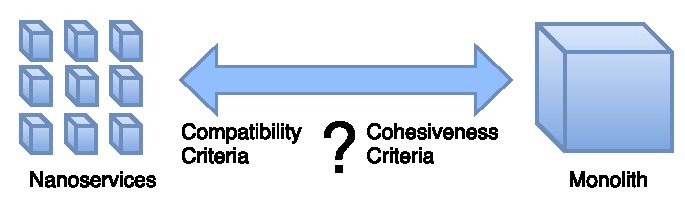
\includegraphics[scale=1]{diagrams/HeuristicApproach.pdf}
	\end{center}
	\caption{Finding a good number of services is a key challenge of service secomposition}
	\label{fig:numberOfServices}
\end{figure}

To simplify the problem for the heuristic approach we assume the number of services is given by the user and does not need to be computed. Very often an architect has a reasonable assumption about the number of services suitable for his system.

The heuristic approach starts with a unordered list of all nanoentities and services that can be imagined as empty boxes that are incrementally filled. The algorithm runs multiple iterations of construction and optimization steps.

\begin{description}
	\item[Construction] Nanoentities are sequentially taken from the list and put in the best suitable service. The target service is calculated by the criteria scores between the selected nanoentity and the nanoentities a service contains at that point of time. 
	\item[Optimization] Within a service the score from each nanoentity to all its neighbors in the same service is calculated to determine the least suitable nanoentity in a service. This nanoentity is taken out of the service and put back on the list of unassigned nanoentities.
\end{description}

%TODO: illsutration?

The algorithm alternates between construction and optimization steps. It finishes either after a given time, by the user stopping the optimization or by detecting that no further optimization is possible. This is detected when nanoentities taken from services in the optimization step are put back to their original service during the construction step.

In an attempt to implement this heuristic approach we realized that even if the algorithm works well, it does not accurately solve the desired problem. The approach focuses only on cohesion within services but does not take coupling between services, that should be minimized, into consideration.

While acceptable results might still be possible using this approach, we decided to focus more on graph clustering due to new findings described in the next section.

\subsection{New Findings on Graph Clustering}

As both alternative approaches did not promise expected results, we shifted our focus back to graph clustering. 

By analyzing the Girvan-Newman algorithm documented in Section \ref{subsec:girvanNewman}, we were able to identify the problem encountered with the booking sample. As the sample only provides \textit{Lifecycle \& Identity Commonality} data, every pair of nanoentities in the graph was either directly or not connected at all. The calculated edge betweenness, which Girvan-Newman is based on, is therefore equal for all edges in the graph as every shortest path only passes one edge. The Gephi\cite{gephi} implementation of Girvan-Newman then consequently removes all edges in the first iteration leaving every nanoentity isolated which then results in one service per nanoentity. Adding only one more information like nanoentity characteristics or use cases solved this problem.

Through further research on the topic we found the algorithm defined by Leung implemented in the GraphStream\cite{leungGraphstream} project and integrated it into the Service Cutter. First tests using the booking sample provided the expected results.

\subsection{Conclusion}

While all approaches possibly lead to the desired results, the new findings on the Girvan-Newman and Leung algorithms promised the best results with adequate effort. Rating possible service cuts or heuristic construction of services would both require great effort. We then decided together with our stakeholders, that it is not worth taking considering that the graph clustering provides reasonable results. 

We furthermore implemented a warning in the Service Cutter should a user provides input leading to the faulty behavior of Girvan-Newman. %TODO implement %
\chapter{Service Cutter Assessment}
\label{testSystems}

We used two example systems to test the Service Cutter. After defining the input used to describe the systems we discussed and documented our expectations on how service decomposition of the systems would make sense from our experience. In order to rate the candidate service cuts provided by the service cutter we defined three categories of cuts:

\begin{description}
	\item[Expected Service Cut] The cut is exactly the way we expected it. 
	\item[Reasonable Service Cut] The cut is not the way we expected it but we find reasons why the cut could make sense from an architects perspective.
	\item[Unreasonable Service Cut] The cut is not as we expected it and we do not find reasons why the cut would provide any benefits to a systems architecture. 
\end{description}

To assess the Service Cutter's output the following language is used:

\begin{itemize}
	\item An \textit{good} output contains zero unreasonable service cuts.
	\item An \textit{acceptable} output contains at most one unreasonable service cut.
	\item A \textit{bad} output contains two or more unreasonable service cuts.
\end{itemize}


\section{Trading System}
\label{sec:tradingSystem}

We developed the Trading System as a fictional example based on personal experience with similar systems. Its goal is to include various different coupling aspects in a rather small model.

The Trading System is an application one might find in a typical swiss private bank offering its customers the ability to manage their stocks portfolio.

\begin{itemize}
\item The main focus is to buy or sell \textit{stocks} at a specific price (\textit{Order.triggerPrice}) using an \textit{order}.
\item \textit{Prices} are frequently imported from a market data provider and upon import of a price, all orders are checked for orders that can be triggered.
\item When an order is executed, an instruction is sent to the market to purchase or sell the stocks. The \textit{PaymentInfo} contains all necessary information to do so. 
\item \textit{News} are imported from an external provider and are linked to a specific stock. They provide valuable, contextual information when using the system. However traders and customers can easily fall back to any online source should this information not be available.
\item \textit{Recommendations} are suggested to the user of the system based on his existing portfolio.
\end{itemize}

Figure \ref{fig:tradingClasses} shows a domain model of the Trading System.

\begin{figure}[H]
	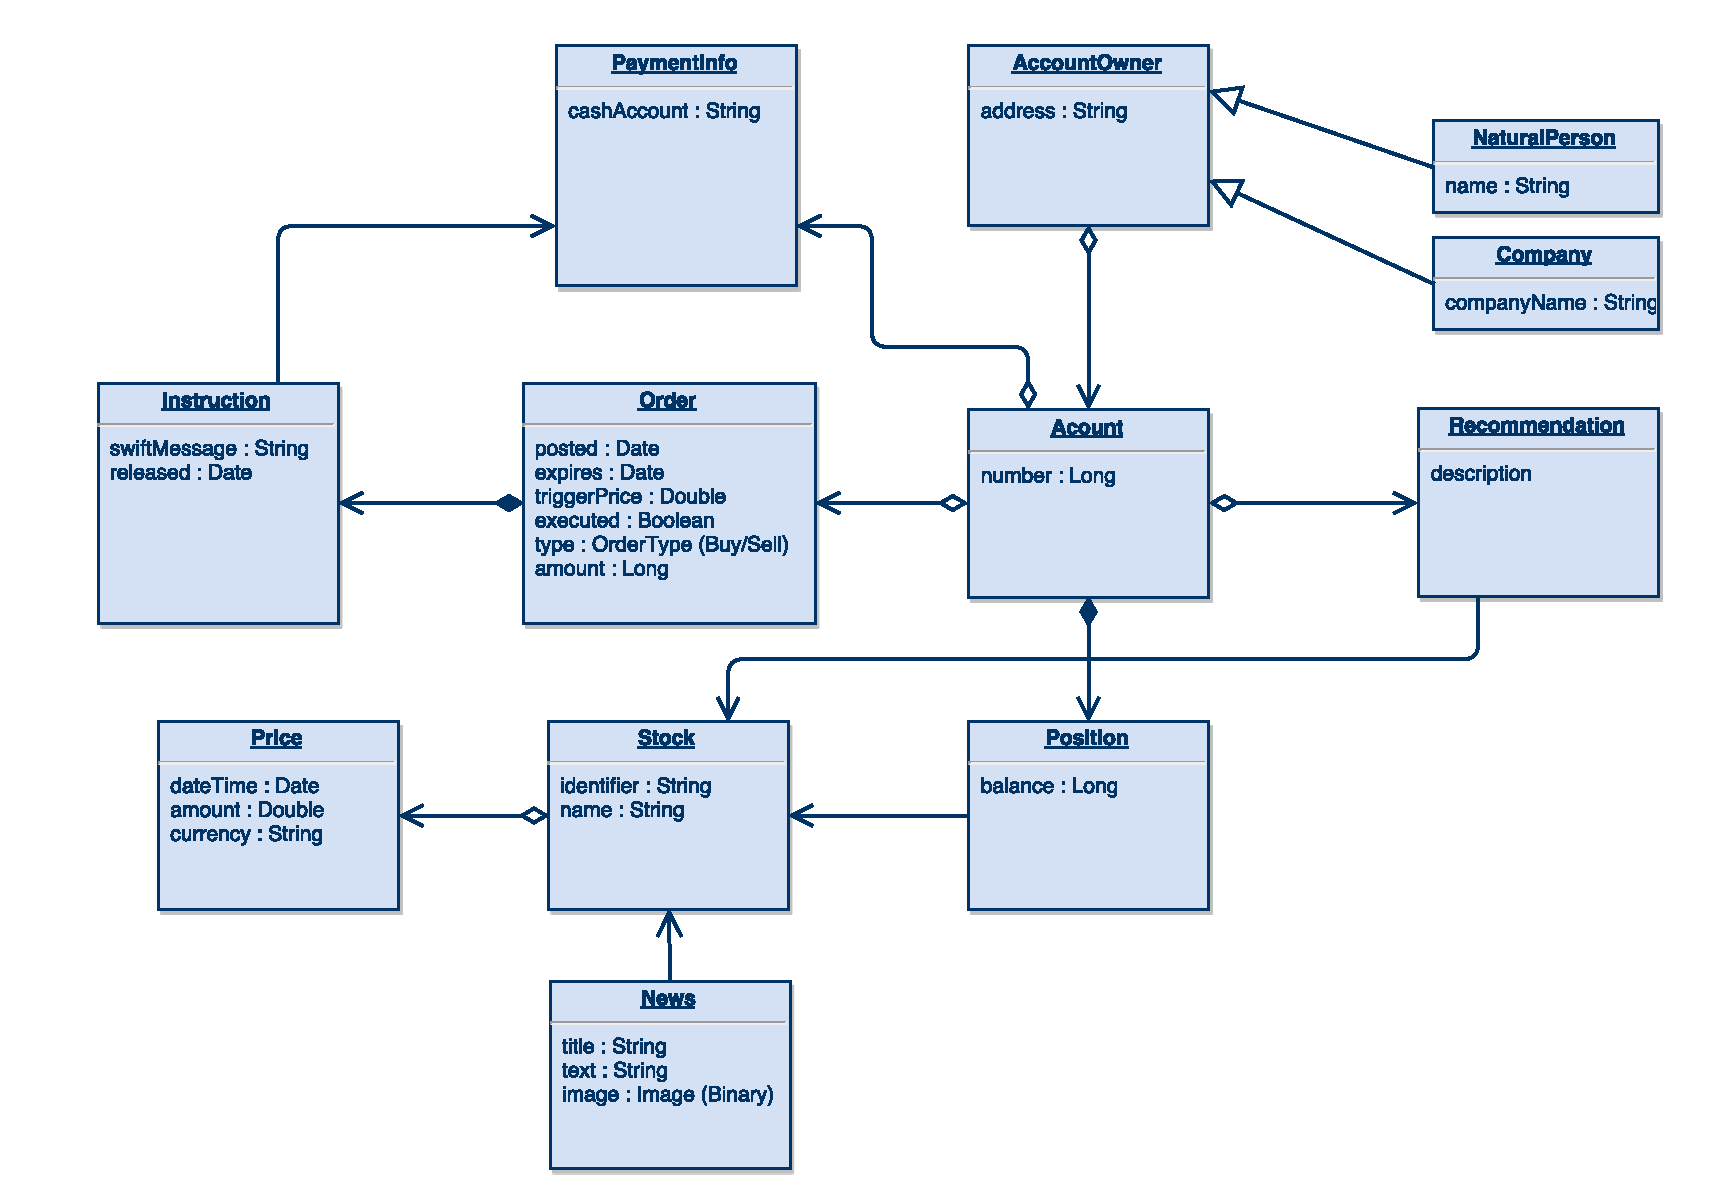
\includegraphics[scale=0.5]{diagrams/TradingSystem.pdf}
	\caption{Trading System Class Diagram}
	\label{fig:tradingClasses}
\end{figure}

The following ten use cases describe the supported functionality of the application.

\begin{enumerate}
\item Post Order
	\begin{itemize}
	\item Nanoentities written: Order.posted,  Order.expires, Order.triggerPrice, Order.executed, Order.type, Order.amount
	\item Nanoentities read: Account.number, Stock.identifier, Stock.stockName
	\end{itemize}
\item Instruct Order
	\begin{itemize}
	\item Nanoentities written: Instruction.instructedTime, Order.executed, Position.balance
	\item Nanoentities read: PaymentInfo.cashAccount
	\end{itemize}
\item Import Price and Check for Due Orders (Technical)
	\begin{itemize}
	\item Nanoentities written: Price.dateTime, Price.price, Price.currency
	\item Nanoentitiess read: Order.triggerPrice, Stock.identifier
	\end{itemize}
\item Read News
	\begin{itemize}
	\item Nanoentities written: - 
	\item Nanoentities read: Stock.identifier, News.title, News.text, News.image
	\end{itemize}
\item Import News (Technical)
	\begin{itemize}
	\item Nanoentities written: News.title, News.text, News.image
	\item Nanoentities read: Stock.identifier
	\end{itemize}
\item View Recommendations
	\begin{itemize}
	\item Nanoentities written: -
	\item Nanoentities read: Account.number, Recommendation.description, Stock.identifier, Stock.stockName
	\end{itemize}
\item Suggest Recommendations (Technical)
	\begin{itemize}
	\item Nanoentities written: Recommendation.description
	\item Nanoentities read: Account.number, Stock.identifier, Stock.stockName, Position.balance
	\end{itemize}
\item Create Account
	\begin{itemize}
	\item Nanoentities written: Account.number
	\item Nanoentities read: AccountOwner.address, NaturalPerson.name, Company.companyName
	\end{itemize}
\item Create Account Owner
	\begin{itemize}
	\item Nanoentities written: AccountOwner.address, NaturalPerson.name, Company.companyName
	\item Nanoentities read: -
	\end{itemize}
\item View Portfolio
	\begin{itemize}
	\item Nanoentities written: -
	\item Nanoentities read: Account.number, Position.balance, Stock.identifier, Stock.stockName, Order.triggerPrice, Order.amount, Order.posted, Order.expires, Order.executed, Order.type
	\end{itemize}
\end{enumerate}

In addition to the use cases, we defined the following characteristics.

\textbf{Security Criticality}

\begin{itemize}
\item \textbf{Critical}: AccountOwner.address, NaturalPerson.name, Company.companyName
\item \textbf{Public}: Stock.identifier,Stock.stockName, Price.dateTime, Price.price, Price.currency, News.title, News.text, News.image
\end{itemize} 

\textbf{Volatility}

\begin{itemize}
\item \textbf{Often}: Price.dateTime, Price.price, Price.currency
\item \textbf{Rarely}: AccountOwner.address, NaturalPerson.name, Company.companyName, Account.number
\end{itemize}

\textbf{Consistency}

\begin{itemize}
\item \textbf{Eventually}: Price.dateTime, Price.price, Price.currency
\end{itemize}

\textbf{Storage Similarity}

\begin{itemize}
\item \textbf{Huge}: News.image
\end{itemize}

\textbf{Change Similarity}

\begin{itemize}
\item \textbf{Often}: Recommendation.description
\end{itemize}

\textbf{Resilience}

\begin{itemize}
\item \textbf{Low}: News.title, News.text, News.image, Recommendation.description
\end{itemize}

Furthermore all default characteristics as documented in Section \ref{sec:couplingCriteria} are taken into account.

\subsection{Expected Service Cuts}

From our experience in software architecture we expect the Service Cutter to decompose the Trading System into the services presented in Figure \ref{fig:tradingCuts}.

\begin{figure}[H]
	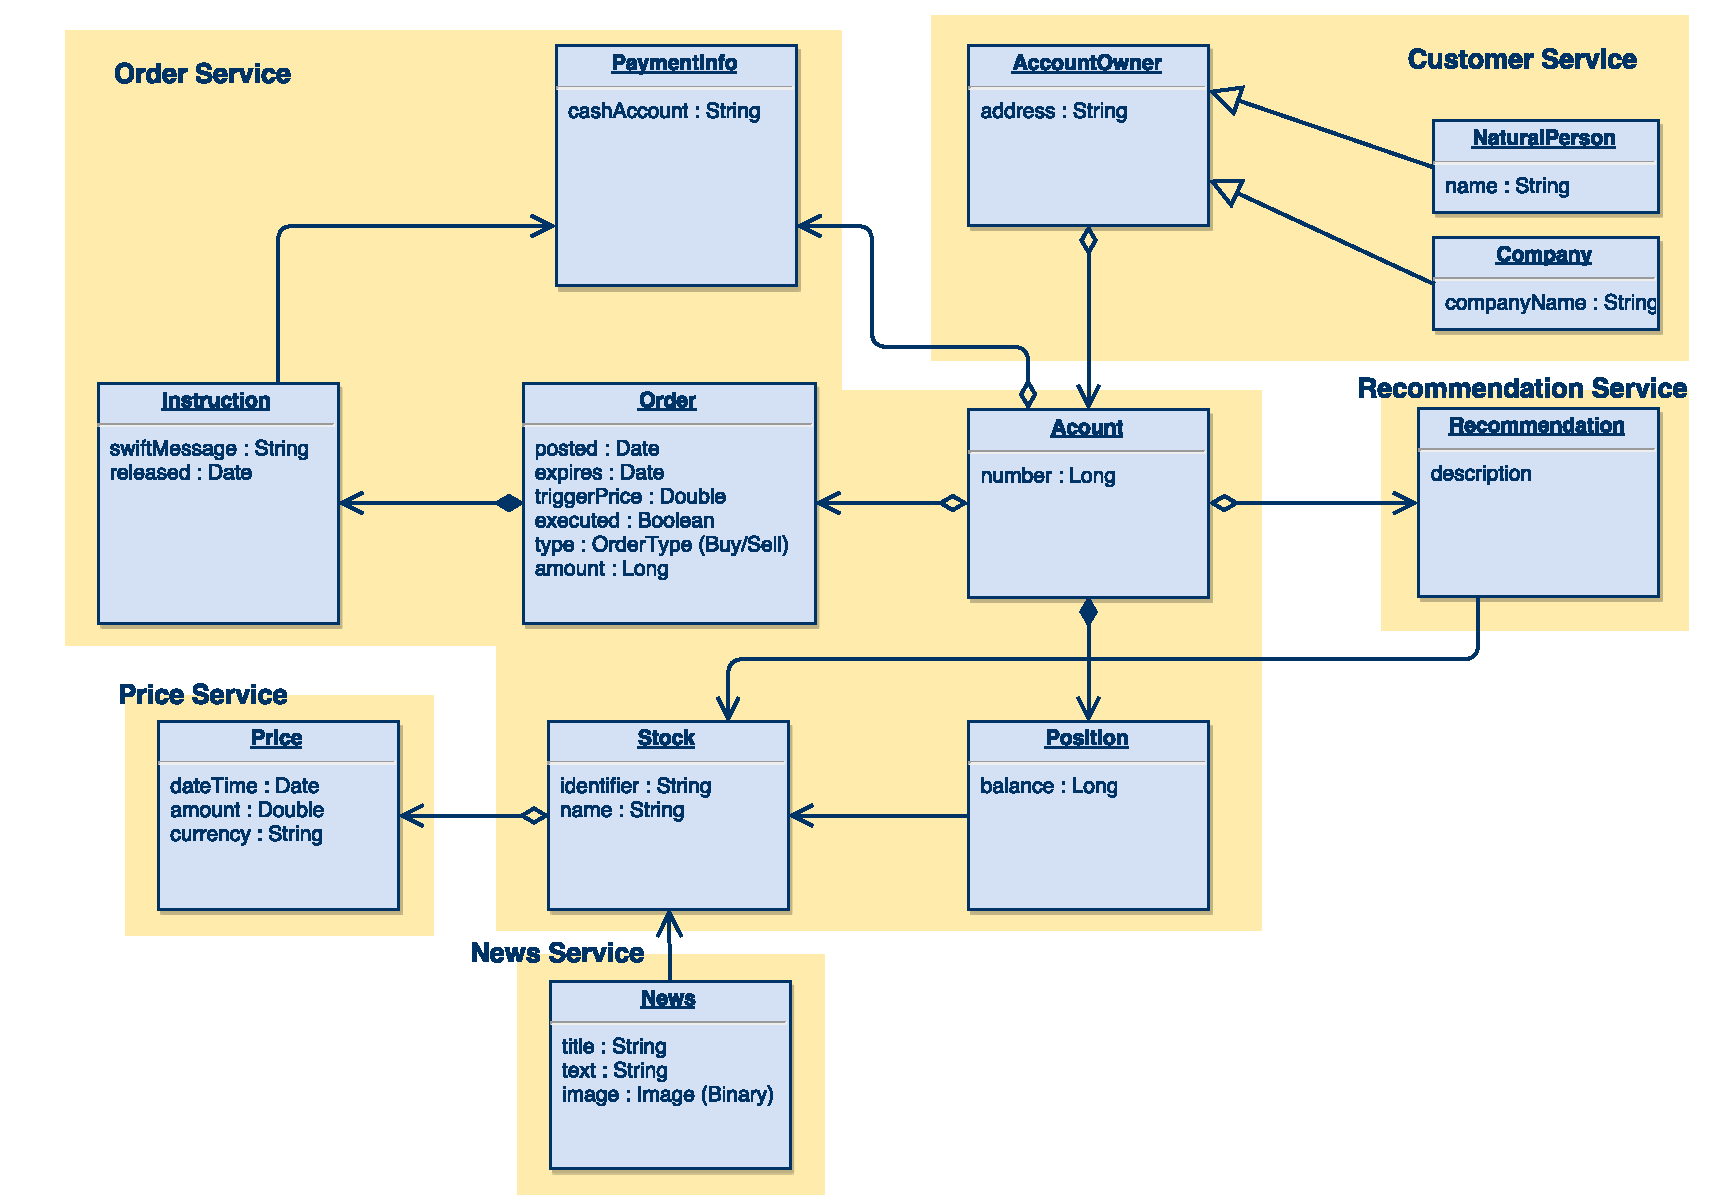
\includegraphics[scale=0.5]{diagrams/TradingSystem-ServiceCut.pdf}
	\caption{Trading System expected service cuts}
	\label{fig:tradingCuts}
\end{figure}

The following reasons led us to this decision.
\begin{itemize}
	\item The service \textit{Order} encapsulates many use cases and contains several entities that need to be processed with high consistency (Order, Position).
	\item The high volatility of the entity price led to the isolation of this part into an own service \textit{Price}.
	\item News are not part of the core operations and therefore require lower resilience and security criticality. News images furthermore require a significant amount of storage. Therefore we would isolate this into a separate \textit{News} service.
	\item The recommendation algorithm will be changed frequently. A dedicated \textit{Recommendation} service allows independent deployment of updated versions. Moreover recommendations are, like the news, not part of the core operations and require lower resilience. 
	\item Security restrictions requires all \gls{PII} to be separated from other data. Extracting it into a \textit{Customer} service allows the architect to protect this data with additional measures. 
\end{itemize}


\subsection{Girvan-Newman Algorithm Assessment}

Figure \ref{fig:tradingCutsTool} is the suggested cut as calculated by the Service Cutter with the Girvan-Newman algorithm. 

\begin{figure}[H]
	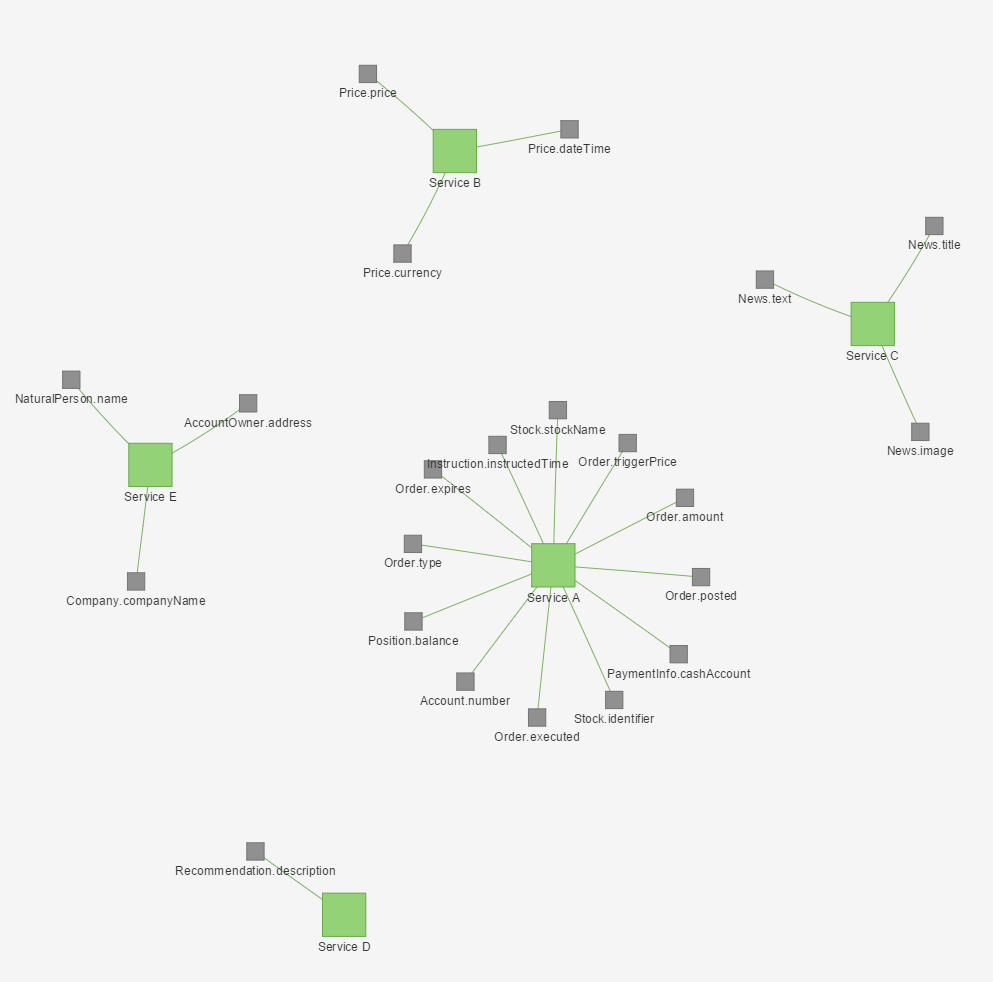
\includegraphics[scale=0.5]{images/trading_service_cut.png}
	\caption{Trading System actual service cuts}
	\label{fig:tradingCutsTool}
\end{figure}

The parameters that produce a cut as seen in \ref{fig:tradingCutsTool} are the following:

\begin{itemize}
\item Coupling criteria priorities: Defaults as defined in \ref{sec:defaultPriorities}
\item Number of services: 5
\end{itemize}

The presented candidate service cuts match exactly the expected services and are therefore considered a good result.

\subsubsection{Priorities Sensitivity}

The candidate service cuts are very stable when changing the priorities. Changing the two relevant cohesiveness parameters \textit{Identity \& Lifecycle Commonality} and \textit{Semantic Proximity} to any combination between \textit{XS} and \textit{L} only affects the result when both set to \textit{L}. With these priorities the Service Cutter suggests an own service for \textit{Stock.stockName} and \textit{Stock.identifier} instead of \textit{Recommendation.description}.

An own service for stocks is reasonable as these nanoentities can be categorized as master data and not transaction data like most of the other nanoentities in the order service. Requesting 6 number of services with these priorities creates cuts for both the recommendation and the stock service. 

Changing the priority of compatibility or constraint criteria to any value between \textit{XS} and \textit{L} does not affect the resulting cuts. However the possibility to request a small number of services gets lost as too many relations between nanoentites are cut if criteria scoring negative values receive a high priority. 

\subsubsection{Number of Services}

As Girvan-Newman receives a number of services parameter we can analyze how a monolithic architecture would be split up step by step. The resulting services by each parameter are listed in Table \ref{tab:tradingNumberOfServices}.

\begin{table}[H]
	\centering
	\caption{Girvan-Newman cuts of trading system with different number of services}
	\label{tab:tradingNumberOfServices}
	\begin{tabular}{|p{60pt}|p{200pt}|}
		\hline	
		\textbf{Number of services} & \textbf{Services}  \\
		\hline
		1 & Monolith \\
		\hline
		2 & Customer Service extracted \\
		\hline
		3 & Price Service extracted  \\
		\hline
		4 & News Service extracted  \\
		\hline
		5 & Recommendation Service extracted  \\
		\hline
		6 & Not supported\\
		\hline
		7 & Payment Service and Instruction Service extracted \\
		\hline
		8 & Stock Service extracted \\
		\hline
		9 & Stock Service splitted in \textit{Stock.name} and \textit{Stock.identifier} \\
		\hline
	\end{tabular}
\end{table}

Reasonable cuts are presented for up to 8 different services. The results produced by Girvan-Newman with the Trading System example are very satisfying as \textit{good} results are presented with almost all combinations of parameters. 

\subsection{Leung Algorithm Assessment}

Leung produces varying suggested cuts as it is not a deterministic algorithm. The algorithm is therefore harder to analyze, as we can't determine if changes in results emerge from changes in priorities or by coincidence. 

Generally speaking the results are similar as those by Girvan-Newman. With the default priorities, the result matches the one of Girvan-Newman shown in Figure \ref{fig:tradingCutsTool} in approximately 50\%. In the cases it is not matching it suggests fewer service by merging two services together. This is due to the label propagation problem described in XXX.
%TODO describe propagation problem in algorithm description. 

\subsubsection{Priorities Sensitivity}

As already mentioned we can't assess the priority sensitivity with Leung. Changing criteria priorities to values from \textit{XS} to \textit{L} has in some cases produced the following results differing from the one shown in Figure \ref{fig:tradingCutsTool}.

\begin{itemize}
	\item An extra service for PaymentInfo.
	\item An extra service for Stock.
	\item An extra service for Account.
	\item A service combining Account, PaymentInfo and Position.
	\item A service combining News and Stock.
\end{itemize}

Except of the last cut we find reasonable justifications for all cases. In fact, combining PaymentInfo, Account and Position into one service seems to be a considerable suggestion we have not thought of before. These entities are closely related to an account while the other entities in the order service are more focused on the trading itself. 

\subsubsection{Number of Services}

The number of services suggested by Leung vary between 2 and 7 services. There is a tendency towards a higher number of services when cohesiveness criteria are prioritized high and compatibility, and constraints criteria are prioritized low. The same applies vice versa. 

With only small changes to the priorities Leung commonly suggests 4 or 5 services which matches with our expectation. %TODO meistens?

\subsection{Conclusion}

In conclusion we can say that the Service Cutter did suggest the Trading System service cuts as we expected. For both algorithms most results can be considered \textit{good} with only one or two exceptions where the result was considered \textit{acceptable}. These are excellent results for a first test of the Service Cutters scoring and algorithms. 

The tests furthermore show the advantages and disadvantages of a deterministic algorithm. Girvan-Newman produced very stable results and nicely shows the path from a monolith to a more service oriented architecture. Leung on the other hand is harder to analyze but provided us more reasonable candidate service cuts we have not considered before. Leung also suggests a reasonable number of services while this consideration completely lies in the responsibility of the user when using Girvan-Newman.

\section{Cargo Tracking System - Domain-Driven Design Sample}
\label{sec:dddSample}

The Cargo Tracking System is a well known software project created to illustrate the concepts and patterns described in the \gls{DDD} book by E. Evans\cite{evans2003domain}. The DDDSample is hosted on Github\cite{dddGithub} and a short screencast on YouTube\cite{dddScreencast} outlines its functionality. 

The Cargo Tracking System provides a domain with a suitable complexity and, unlike the Trading System, comes with a already implemented and well reasoned architecture. With reverse engineering we extracted the domain model, use cases and some characteristics from the code. The Cargo Tracking implements the following functionalities:

\begin{itemize}
	\item The main focus is to transport a \textit{Cargo} from \textit{Location} A to \textit{Location} B. \textit{Cargos} are created with a \textit{TrackingId} and specified with a \textit{RouteSpecification}. Once created, one of multiple suitable \textit{Itinerarys} is assigned.
	\item The system calculates suitable \textit{Itinerarys} for a \textit{Cargo} from existing \textit{Voyages} each containing a list of \textit{CarrierMovements}.
	\item Once a \textit{Cargo} is routed, \textit{HandlingEvents} track the progress of each \textit{Cargo's} \textit{Itinerary}. A \textit{HandlingEvent} contains information about the event and references a \textit{Cargo} on a specific \textit{Voyage} and occurs in a particular \textit{Location}. 
	\item The \textit{Delivery} of a \textit{Cargo} informs about its state, estimated arrival time and contains information whether the \textit{Cargo} is on track or not.
\end{itemize}

The extracted domain model is not a one-to-one copy of the domain classes in the code. The domain classes contain some calculated and therefore redundant information which have been merged into single nanoentities in the domain model shown in Figure \ref{fig:dddSampleAggregates}. 

\begin{figure}[H]
	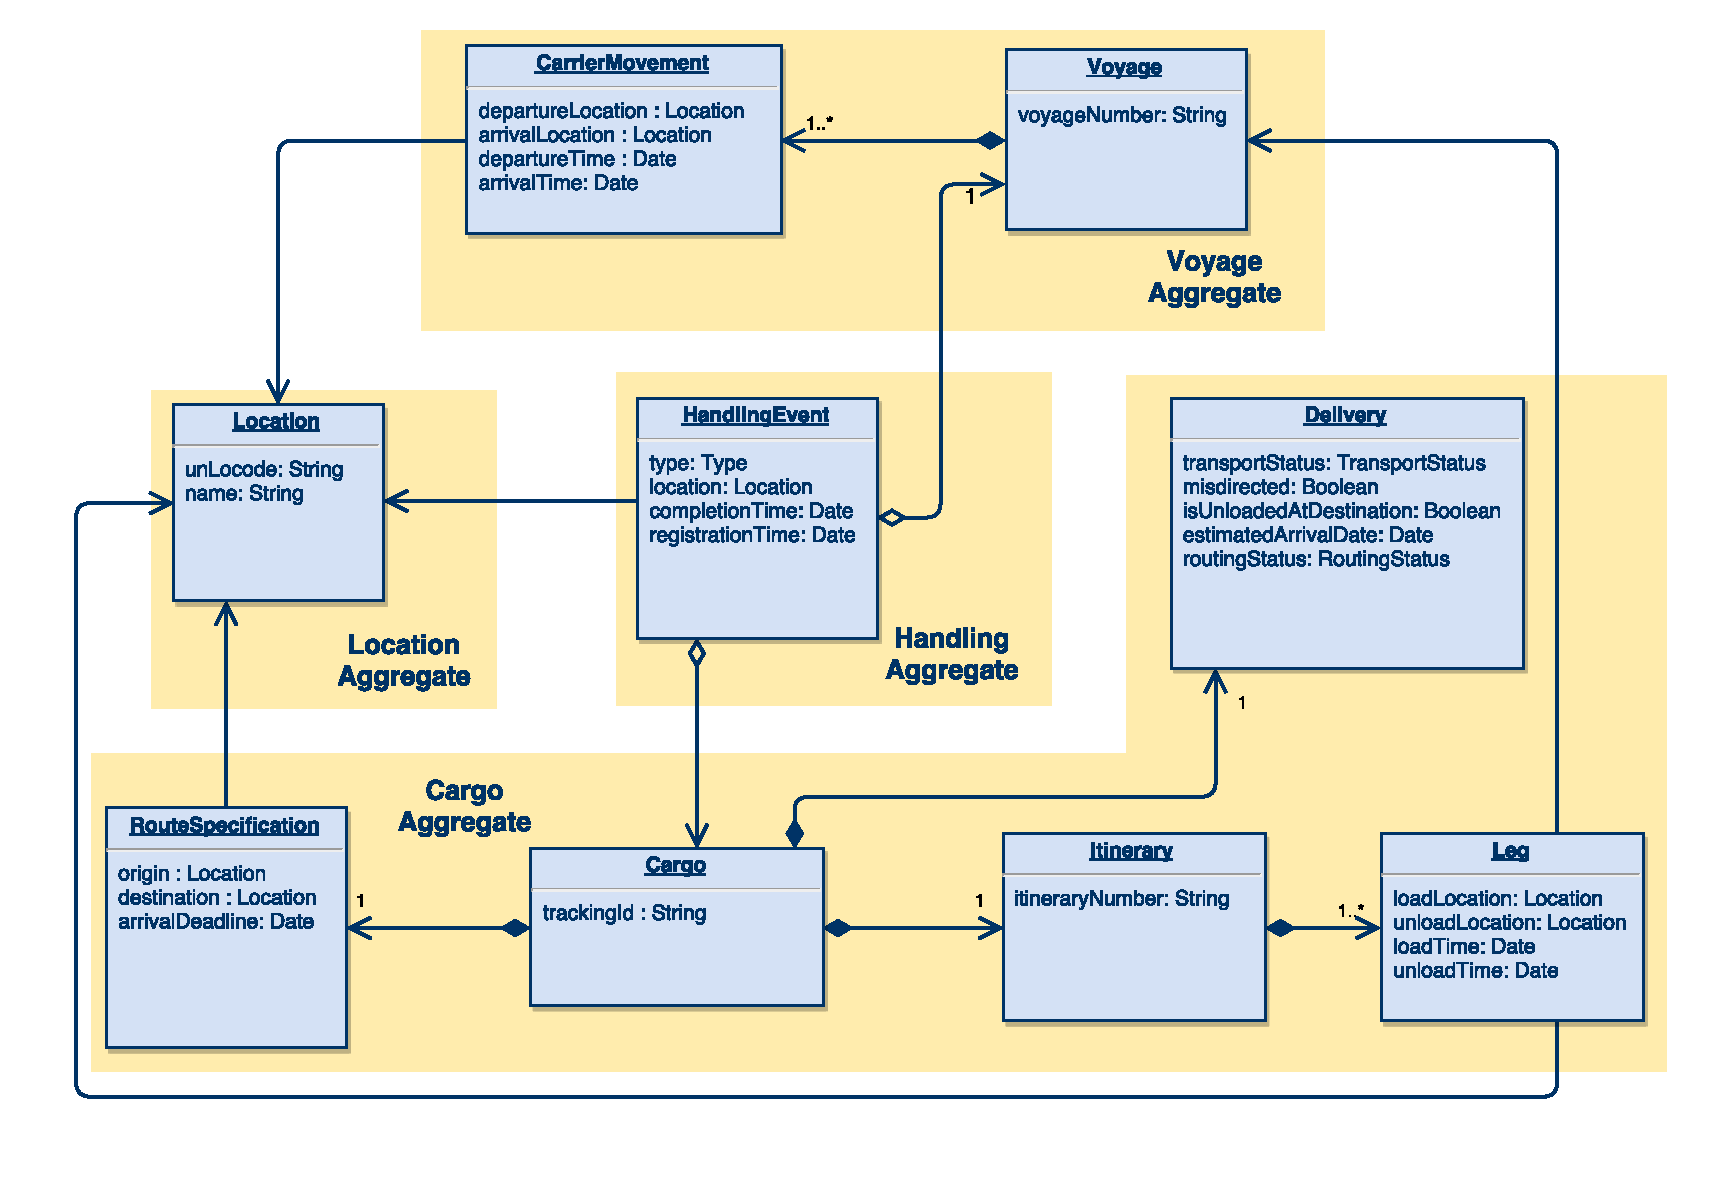
\includegraphics[scale=0.5]{diagrams/ddd_sample_aggregates.pdf}
	\caption{DDD Sample with Aggregates}
	\label{fig:dddSampleAggregates}
\end{figure}

Figure \ref{fig:dddSampleAggregates} additionally outlines the package and aggregate structure provided by the DDDSample which is a first indication about service decomposition. 

The following use cases describe the supported functionality of the application.

\begin{enumerate}
	\item ViewTracking
	\begin{itemize}
		\item Nanoentities written: -
		\item Nanoentities read: Cargo.trackingId, HandlingEvent.type, HandlingEvent.location, HandlingEvent.completionTime, Delivery.transportStatus, Delivery.estimatedArrivalTime, Delivery.misdirected, Voyage.voyageNumber, RouteSpecification.destination, Stock.stockName
	\end{itemize}
	
	\item ViewCargos
	\begin{itemize}
		\item Nanoentities written: -
		\item Nanoentities read: Cargo.trackingId, RouteSpecification.destination, RouteSpecification.arrivalDeadline, Delivery.routingStatus, Itinerary.itineraryNumber
	\end{itemize}
	
	\item BookCargo
	\begin{itemize}
		\item Nanoentities written: Cargo.trackingId, RouteSpecification.origin, RouteSpecification.arrivalDeadline, RouteSpecification.destination
		\item Nanoentities read: Location.unLocode
	\end{itemize}
	
	\item ChangeCargoDestination
	\begin{itemize}
		\item Nanoentities written: RouteSpecification.destination
		\item Nanoentities read: Cargo.trackingId, RouteSpecification.destination
	\end{itemize}
	
	\item RouteCargo
	\begin{itemize}
		\item Nanoentities written: Itinerary.itineraryNumber, Leg.loadLocation, Leg.unloadLocation, Leg.loadTime, Leg.unloadTime
		\item Nanoentities read: Cargo.trackingId, RouteSpecification.destination, RouteSpecification.origin, RouteSpecification.arrivalDeadline, Location.unLocode, Voyage.voyageNumber, CarrierMovement.departureLocation, CarrierMovement.arrivalLocation, CarrierMovement.departureTime, CarrierMovement.arrivalTime
	\end{itemize}
	
	\item Create Location
	\begin{itemize}
		\item Nanoentities written: Location.unLocode, Location.name
		\item Nanoentities read: -
	\end{itemize}

	\item Create Voyage
	\begin{itemize}
		\item Nanoentities written: Voyage.voyageNumber
		\item Nanoentities read: -
	\end{itemize}
	
	\item Add CarrierMovement
	\begin{itemize}
		\item Nanoentities written: CarrierMovement.departureLocation, CarrierMovement.arrivalLocation, CarrierMovement.departureTime, CarrierMovement.arrivalTime
		\item Nanoentities read: Voyage.voyageNumber
	\end{itemize}
	
	\item Handle Cargo Event
	\begin{itemize}
		\item Nanoentities written: HandlingEvent.type, HandlingEvent.completionTime, HandlingEvent.registrationTime, HandlingEvent.location, Delivery.transportStatus, Delivery.misdirected, Delivery.estimatedArrivalTime, Delivery.isUnloadedAtDestination, Delivery.routingStatus
		\item Nanoentities read: Voyage.voyageNumber, Cargo.trackingId
	\end{itemize}
\end{enumerate}

In addition to the use cases, we identified the following characteristics.

\textbf{Volatility}

\begin{itemize}
	\item \textbf{Often}: HandlingEvent.type, HandlingEvent.completionTime, HandlingEvent.registrationTime, HandlingEvent.location, Delivery.transportStatus 
	\item \textbf{Rarely}: Location.unLocode, Location.name
\end{itemize} 

\textbf{Change Similarity}

\begin{itemize}
	\item \textbf{Rarely}: Location.unLocode, Location.name
\end{itemize}

Furthermore all default characteristics as documented in Section \ref{sec:couplingCriteria} are taken into account.

The DDDSample provides multiple interfaces depending on the user's role. The main interface provides tracking information, the administration panel offers means to create cargos and plan their itinerary and an additional interface is used to inform about handling events. Out of these distinction by the \gls{UI} we defined responsibility areas listed in Table \ref{tab:dddResponsibilites} each containing a group of nanoentities a user role is responsible for.

\begin{table}[H]
	\centering
	\caption{Responsibility Areas in DDDSample}
	\label{tab:dddResponsibilites}
	\begin{tabular}{|p{90pt}|p{200pt}|}
		\hline	
		\textbf{Responsibility Area} & \textbf{Nanoentities}  \\
		\hline
		Cargoplaner & Cargo.trackingId \newline RouteSpecification.origin\newline RouteSpecification.destination\newline RouteSpecification.arrivalDeadline\newline Itinerary.itineraryNumber\newline Leg.loadLocation\newline Leg.unloadLocation\newline Leg.loadTime\newline Leg.unloadTime\newline Delivery.estimatedArrivalTime\newline Delivery.routingStatus  \\
		\hline
		CargoTracker & HandlingEvent.type\newline HandlingEvent.completionTime\newline HandlingEvent.registrationTime\newline HandlingEvent.location\newline Delivery.transportStatus\newline Delivery.misdirected\newline Delivery.isUnloadedAtDestination  \\
		\hline
		VoyageManager & Voyage.voyageNumber\newline CarrierMovement.departureLocation\newline CarrierMovement.arrivalLocation\newline CarrierMovement.departureTime\newline CarrierMovement.arrivalTime \\
		\hline
		Admin & Location.name, Location.unLocode \\
		\hline
	\end{tabular}
\end{table}

\subsection{Expected Service Cuts}

From our experience in software architecture we expect the Service Cutter to decompose the Cargo Tracking System into the services presented in Figure \ref{fig:dddSampleServices}.

\begin{figure}[H]
	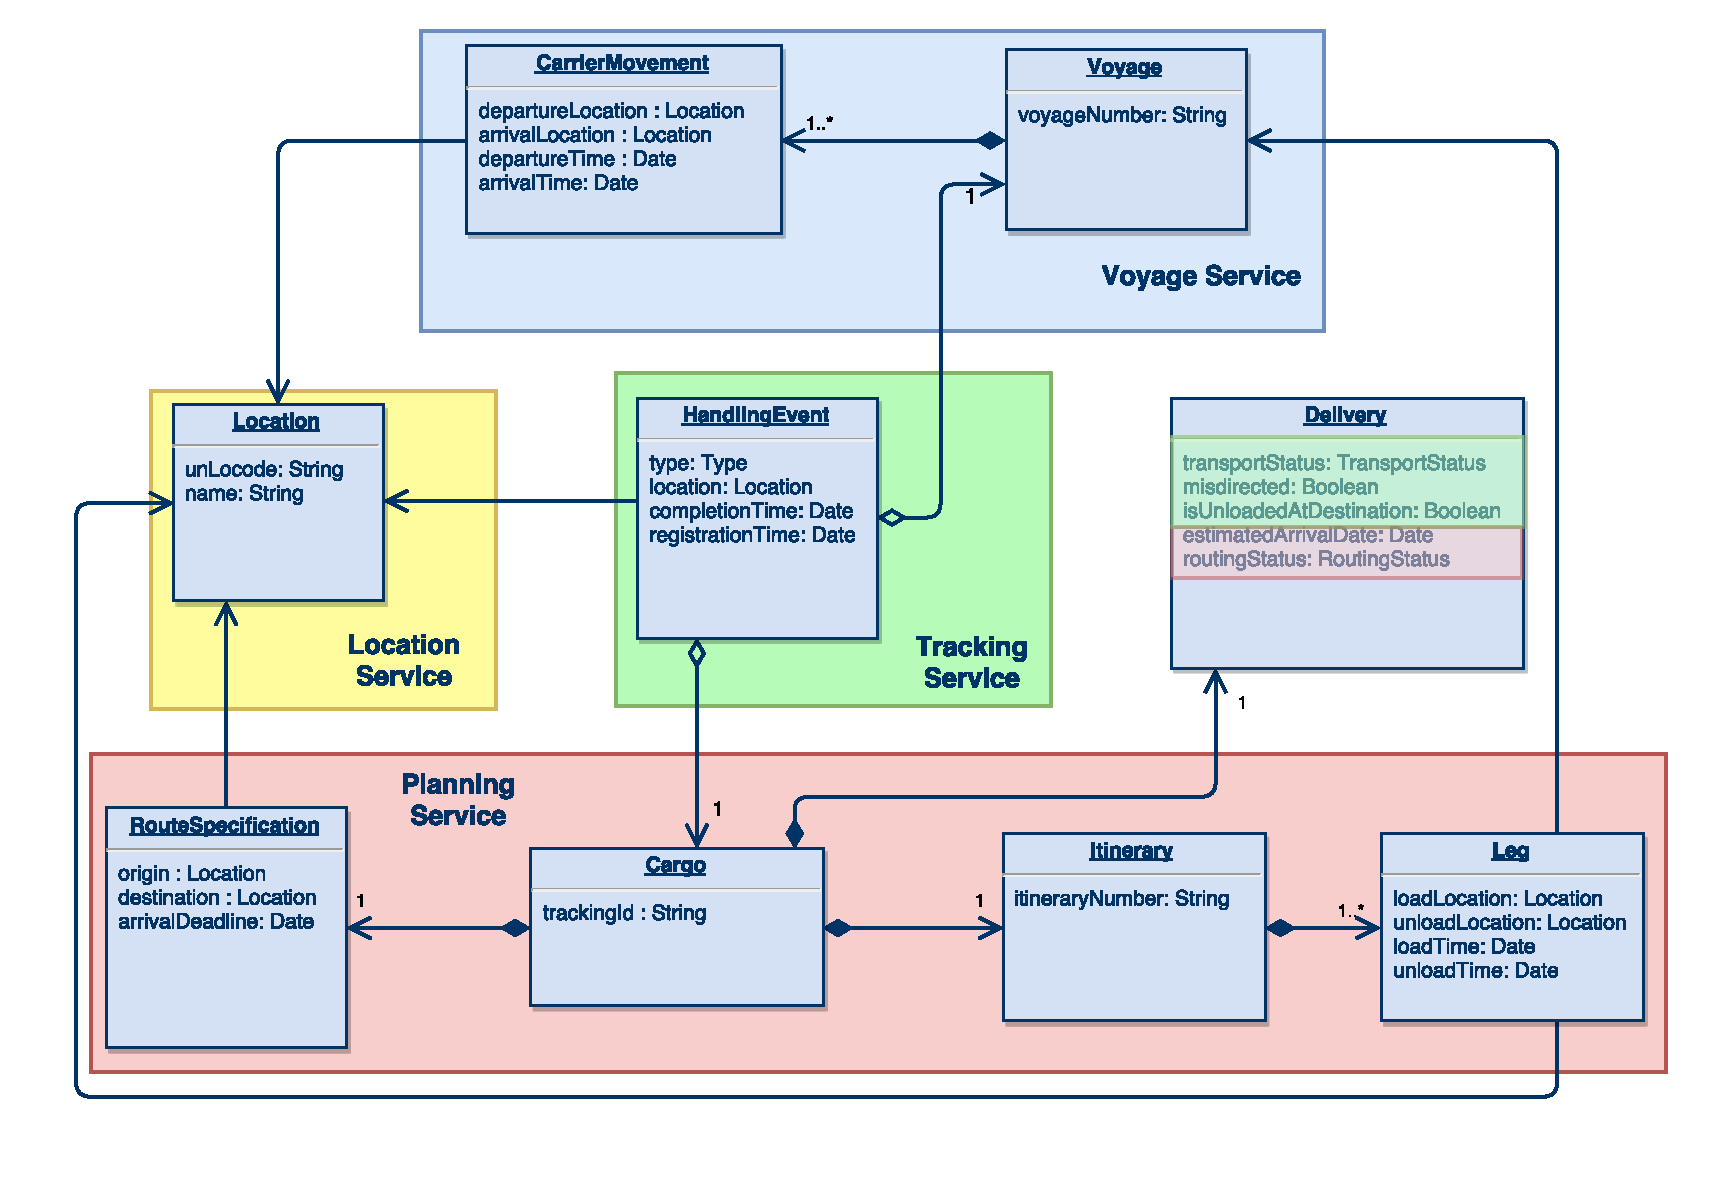
\includegraphics[scale=0.5]{diagrams/ddd_sample_services.pdf}
	\caption{DDD Sample with expected services}
	\label{fig:dddSampleServices}
\end{figure}

As there are not many compatibility criteria defined, the main reasons for our decomposition solution are responsibilities and semantic proximity by use cases:

\begin{itemize}
	\item The \textit{Voyage Service} contains all nanoentities regarding actual voyages and their movements, regardless of any cargo. 
	\item The \textit{Location Service} is separated as a consequence of the low volatility and change similarity of these nanoentities. Locations are used and referred from almost all entities but very rarely written. This service could be categorized as a master data service.
	\item The \textit{Planning Service} handles all nanoentities regarding cargos and their itinerary. 
	\item The \textit{Tracking Service} is responsible to track the actual events of a cargo. The aggregates defined in the DDDSample assign the delivery to the Planning Service. In our opinion the nanoentities \textit{transportStatus}, \textit{misdirected} and \textit{isUnloadedAtLocation} are better assigned to the Tracking Service as they are defined as a consequence of handling events.
\end{itemize}

\subsection{Girvan-Newman Algorithm Assessemnt}

For the Cargo Tracking System the default priorities were adjusted to the following values:

\begin{itemize}
	\item Volatility: \textit{S} instead of \textit{XS}
	\item Change Similarity: \textit{S} instead of \textit{XS}
	\item Responsibility: \textit{L} instead of \textit{M}
\end{itemize}

The resulting candidate service cuts by the Girvan-Newman algorithm for 4 services are shown in Figure \ref{fig:dddGirvanNewman}.

\begin{figure}[H]
	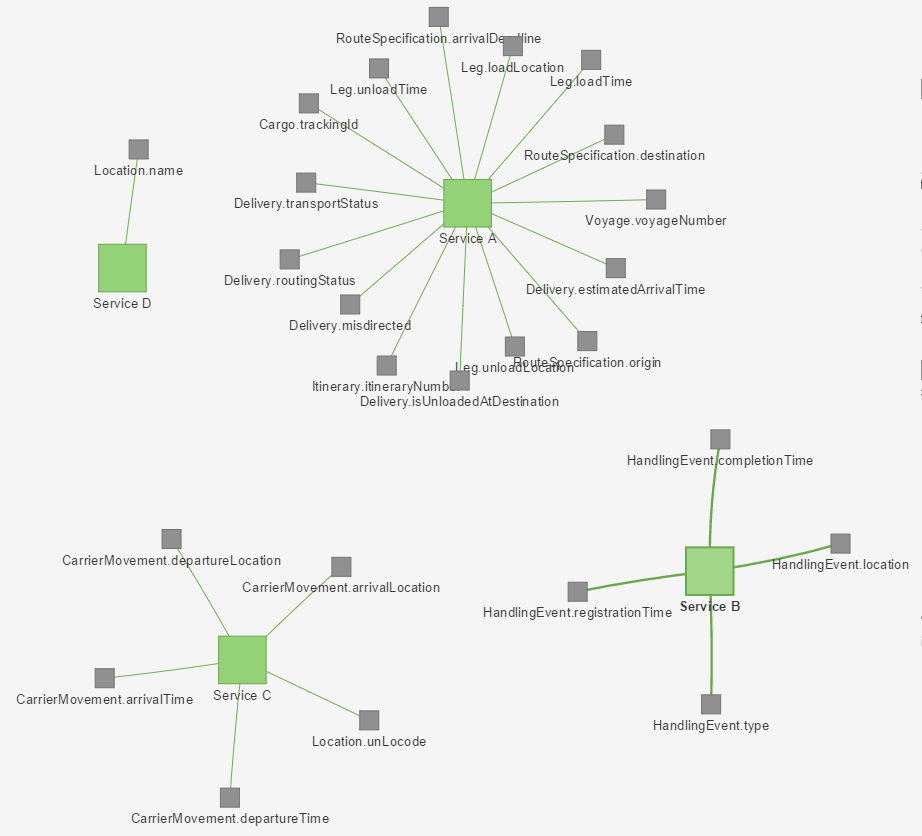
\includegraphics[scale=0.7]{images/ddd_girvan_4.png}
	\caption{Cargo Tracking System Service Cuts by Girvan-Newman}
	\label{fig:dddGirvanNewman}
\end{figure}

Surprisingly, the location has been split to Service D and Service C. Service C contains the carrierMovement nanoentities but misses the voyageNumber which is closely related to the carrierMovement through responsibilities and use cases. Service B represents the handling aggregate as defined by the DDDSample but does not contain delivery nanoentites as expected by us. 

None of the service contains the nanoentities as expected by us and only Service B can be categorized as reasonable service cut. We rate this a \textit{bad} result. 

The split of location might be due to the fact that in most use cases only Location.unLocode is used and not Location.name. We changed the priority for \textit{Semantic Proximity} from \textit{M} to \textit{S} which resulted in the candidate service cuts shown in Figure \ref{fig:dddGirvanNewmanS}

\begin{figure}[H]
	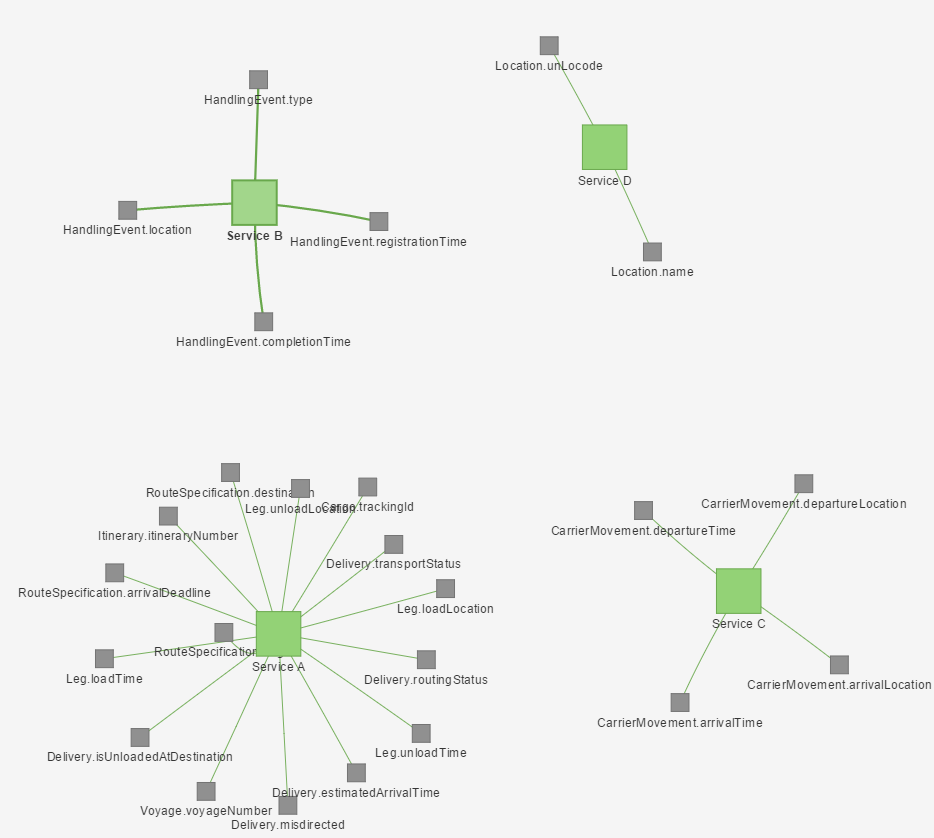
\includegraphics[scale=0.7]{images/ddd_girvan_4_proximity_s.png}
	\caption{Semantic Proximity with Priority S instead of M}
	\label{fig:dddGirvanNewmanS}
\end{figure}

Location has now an own service as expected. This improves the result a little but still not enough to consider it \textit{acceptable}.

\subsubsection{Priorities Sensitivity}

Changing priorities of the relevant coupling criteria to values between \textit{XS} and \textit{L} results in minor changes. The following alternations have been produced:

\begin{itemize}
	\item Delivery.transportStatus is assigned to the service containing handling events if \textit{Identity \&Lifecycle Commonality} is set to \textit{XS}. This is closer to our expectation of a tracking service.
	\item Increasing the priority of \textit{Semantic Proximity} to \textit{L} produces an unreasonable service containing Cargo, Voyage and RouteSpecification nanoentities.
\end{itemize}

We were not able to produce \textit{acceptable} or \textit{good} results for the Cargo Tracking System with Girvan-Newman. The sensitivity of the results on priority changes seems acceptable. 

\subsection{Leung Algorithm Assessment}

Like Girvan-Newman, the Leung algorithm only suggests a location service if \textit{Semantic Proximity} is set to \textit{S} instead of \textit{M}. The candidate service cuts are shown in Figure \ref{fig:dddleungVoyage}.	

\begin{figure}[H]
	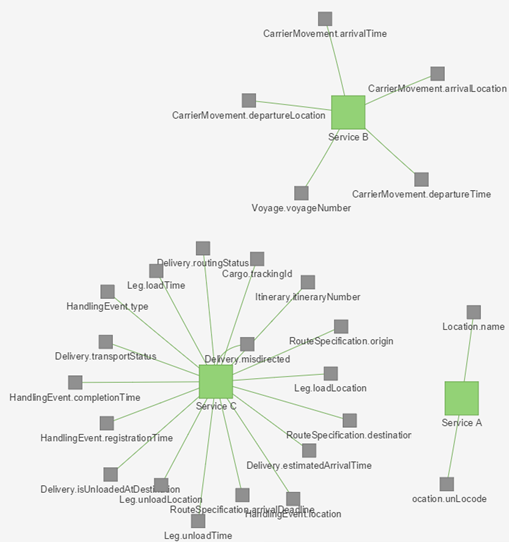
\includegraphics[scale=0.9]{images/leung_voyage.png}
	\caption{Cargo Tracking System Service Cuts by Leung}
	\label{fig:dddleungVoyage}
\end{figure}

A location and a voyage service have been extracted while the planning and tracking service are merged together. A different run with the same priorities is shown in Figure \ref{fig:dddleungTracking}.

\begin{figure}[H]
	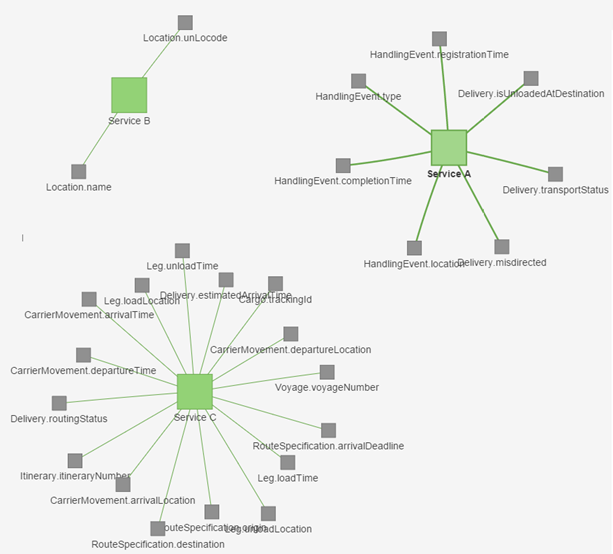
\includegraphics[scale=0.9]{images/leung_tracking.png}
	\caption{Cargo Tracking System Service Cuts by Leung}
	\label{fig:dddleungTracking}
\end{figure}

This time Leung extracted the tracking service and kept voyage and planning services together. Noteworthy is the fact that Leung splits the delivery entity in two different services the same way we expected it. 

Other runs resulted in similar cuts whereas often only the location service was extracted. The cuts done by Leung meet our expectations precisely but provides less services than expected. We assume this results from the label propagation problem described in Section XX. 
%TODO: describe Leung problem. 

The results provided by Leung can be classified as \textit{acceptable}.









 %
\chapter{Clustering Graph Evaluation}
\label{appendix:graphClustering}

To implement the graph approach described in Section \ref{subsec:approach1_graph}, a clustering algorithm is required to split the undirected weighted graph into as little as possible connected groups of data fields. 

The requirements listed in Table \ref{tab:requirementsAlgorithm} should be met by the algorithm and it's implementation:

\begin{table}[H]
	\centering
	\caption{Algorithm Requirements}
	\label{tab:requirementsAlgorithm}
	\begin{tabular}{|p{100pt}|p{250pt}|p{50pt}|}
		\hline	
		Name & Description & Priority \\
		\hline
		Distinct Clusters & Every field is contained once and only once in a cluster. & High  \\
		\hline
		Balanced Coupling & The sum of weights of the edges a cluster connects with other clusters should be similar for all clusters. & High \\
		\hline
		Minimal Coupling & The total weight of the edges connecting clusters should be minimal. & High \\
		\hline
		Implementation & A free implementation of the algorithm should be available either in Java or another language easily callable from the \gls{JVM}. & High  \\
		\hline
		Number of Clusters & The number of clusters should be defined by a parameter. & Medium \\
		\hline
		Performance & An algorithm run with 2000 edges should not take longer than 2 minutes on an average laptop. & Medium \\
		\hline
		Simplicity & It should be possible to understand the mechanism and parameters of the algorithm within a day with the mathematical background we have from the studies at \gls{HSR}. & Low \\
		\hline
		%TODO: specify more
		Hardship Cases & Cases in which it is unclear which cut is best should be made visible in form of a hint or multiple solution suggestions. & Low \\
		\hline
		License & ? & ? \\
		\hline
	\end{tabular}
\end{table}

The algorithms listed in Table \ref{tab:algorithmEvaluation} are the result of a online research on clustering and community algorithms.

\begin{table}[H]
	\centering
	\caption{Algorithm Evaluation}
	\label{tab:algorithmEvaluation}
	\begin{tabular}{|p{90pt}|p{200pt}|p{130pt}|}
		\hline	
		Name & Description & Implementation \\
		\hline
		MCL - Markov Cluster Algorithm\cite{mcl} & A clustering algorithm working on weighted undirected graphs. MCL is based on Random Walks with Markov Chains. & Implementations of MCL are available in R and in Java as s plugin of the Gephi\cite{gephi} platform.  \\
		\hline
		HCS - Highly Connected Subgraphs\cite{hcs} & A clustering algorithm working on unweighted undirected graphs. The CLICK clustering algorithm enhances HCS for weighted edges. & Implementations only available in R.  \\
		%TODO: check CLICK algorithm again
		\hline
		Girvan–Newman\cite{girvanNewman} & A clustering algorithm working on weighted undirected graphs based on Edge-Betweenness \footnote{The amount of shortest paths between nodes going through a specific edge.}. & Java implementations exist as part of the Jung\cite{jung} framework (only unweighted graphs) and as a plugin of the Gephi\cite{gephi} platform. \\
		\hline	
		K-means\cite{kmeans} & A clustering algorithm working with vectors in an n-dimensional space. & Multiple implementations, for example as part of the Spark\cite{spark} framework, are available. \\
		\hline
		Apiacoa\cite{apiacoa} & A clustering algorithm working on unweighted undirected graphs. This algorithm is based on maximal modularity clustering. & Apiacoa.com provides an implementation of the algorithm in Java. \\
		\hline
		%TODO: what is maximal modularity clusterni?	
		%TODO: replace wikipedia with original sources		
	\end{tabular}
\end{table}

We did not find a simple way to transform the problem from a graph to vector based representation in order to use k-means as a solution. We  decided to try the Gephi implementations of Girvan-Newman and MCL as Apiacoa does not support weighted edges and no Java implementation for HCS was found. Gephi is a desktop platform with a well developed \gls{UI} to explore and visualize complex graphs and network systems. The two algorithms are provided by Gephi plugins, from which the algorithm implementations can be extracted as \gls{JAR} files. 
	% 
\chapter{Implementation Details}
\label{appendix:implementationDetails}

This appendix contains detail documentation, code, or configuration files used to implement the Service Cutter.

\section{JSON Schema Export}
\label{appendix:exportSchema}

Listing \ref{code:exportSchema} lists the JSON Schema that specifies the export format for candidate service cuts.

\lstset{
	language=JavaScript,
	tabsize=3,
	%frame=lines,
	caption=JSON Schema for candidate services export.,
	label=code:exportSchema,
	frame=shadowbox,
	rulesepcolor=\color{gray},
	xleftmargin=20pt,
	framexleftmargin=15pt,
	keywordstyle=\color{blue}\bf,
	commentstyle=\color{OliveGreen},
	stringstyle=\color{red},
	numbers=left,
	numberstyle=\tiny,
	numbersep=5pt,
	breaklines=true,
	showstringspaces=false,
	basicstyle=\footnotesize}
\lstinputlisting{code/JSONSchema_export.json}

\section{Docker Compose}
\label{appendix:dockerCompose}

A \gls{yaml} file is used to configure and start all Docker containers required for the Service Cutter. The file shown in Listing \ref{code:dockercompose} is delivered as \texttt{docker-compose.yml} in the source code of the Service Cutter.

In a productive environment the default passwords as defined in the Docker Compose file have to be changed.

\lstset{
   	language=,
   	tabsize=3,
   	%frame=lines,
   	caption=Docker Compose definition for the Service Cutter,
   	label=code:dockercompose,
   	frame=shadowbox,
   	rulesepcolor=\color{gray},
   	xleftmargin=20pt,
   	framexleftmargin=15pt,
   	keywordstyle=\color{blue}\bf,
   	commentstyle=\color{OliveGreen},
   	stringstyle=\color{red},
   	numbers=left,
   	numberstyle=\tiny,
   	numbersep=5pt,
   	breaklines=true,
   	showstringspaces=false,
   	basicstyle=\footnotesize}
\lstinputlisting{code/docker-compose.yml}
 % 

\chapter{Project Management}
\label{cha:projectmgmt}

This Appendix documents aspects of project management like methodology, roles, environment, quality management, and risk management. The project was time boxed and started on \formatdate{14}{9}{2015} and ended on \formatdate{18}{12}{2015} which implies 14 working weeks. 

\section{Milestones}

Apart from the appointed project end on the \formatdate{18}{12}{2015}, the following milestones ensure a timely progress.

\begin{enumerate}
\item \textbf{\formatdate{23}{10}{2015}} - Finished chapters "Context", "Idea" and "Requirements"
\item \textbf{\formatdate{20}{11}{2015}} - Finished chapters "Solution / Architecture / Design"
\item \textbf{\formatdate{14}{12}{2015}} - Finished chapters "Result", "Discussion" and "Future Work"
\end{enumerate}

All milestones relate to the documentation. The coding tasks are scheduled to be mostly finished with the milestone 2 as well. A more detailed breakdown is presented in Appendix \ref{sec:projplan}.
\section{Sprint Plan}
\label{sec:projplan}

The project is organized in 4 regular sprints with each two weeks length. 

\begin{itemize}
\item 1st Sprint: \formatdate{14}{09}{2015} - \formatdate{25}{09}{2015}
\subitem Refinement of thesis concept
\subitem Implementation of prototype
\item 2nd Sprint: \formatdate{12}{10}{2015} - \formatdate{23}{10}{2015}
\subitem Development of algorithm
\subitem Development of Coupling Criteria catalog
\item 3rd Sprint: \formatdate{09}{11}{2015} - \formatdate{20}{11}{2015}
\subitem Finish functional requirements
\subitem Test significantly large project
\item 4th Sprint: \formatdate{30}{11}{2015} - \formatdate{11}{12}{2015}
\subitem Refine scoring system, fine tune sample models
\item 5th Sprint: \formatdate{14}{12}{2015} - \formatdate{18}{12}{2015} (one week)
\end{itemize}

The 5th sprint will solely be used to finish the documentation.

%TODO müssen wir beschreiben, was wir zwischen den sprints machen?

\section{Hours Worked}

We invested a total of 757 hours on this project. Michael Gysel worked 365 hours and Lukas Kölbener spent 392 hours on this thesis. Figure \ref{fig:hoursworked} breaks these numbers down into individual categories. We tracked them using epics which is a common technique in agile projects.

\begin{figure}[H]
	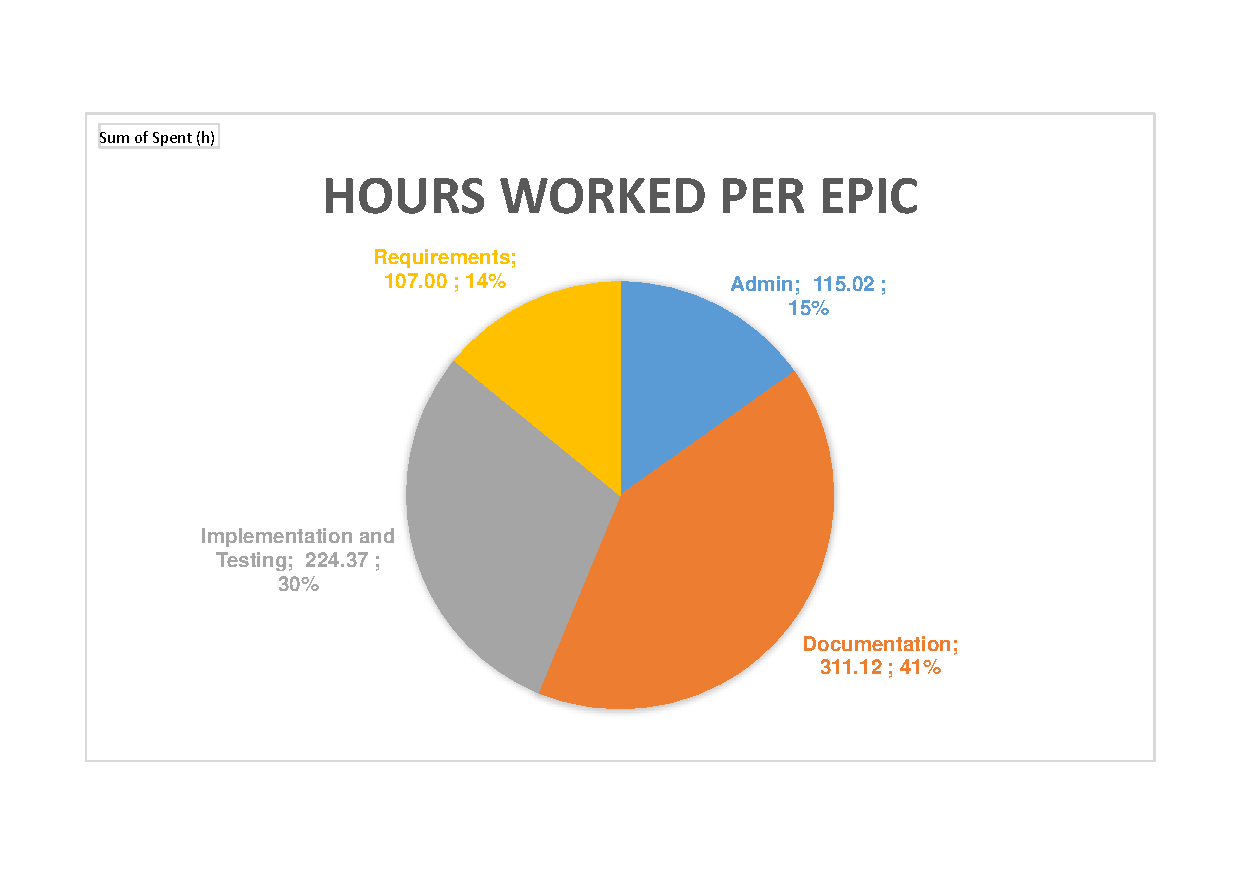
\includegraphics[scale=0.7]{diagrams/hoursperepic.pdf}
	\caption{Development Environment}
	\label{fig:hoursworked}
\end{figure}
\section{Risk Management}

%TODO: we should have a measurement for impact and "Eintretungswahrscheinlichkeit" to provide a proper risk mgmt analysis.

To assess the risk associated with this project, a comprehensive list of possible risks and their mitigations is described in the following Section. 

The risk assessment shown in Table \ref{tab:toprisks} is based on a literature survey\cite{risk} taken in 2011. Two custom lists of project specific risks are documented in Table \ref{tab:projmgmtrisks} and Table \ref{tab:projtechnicalrisks}.

\begin{table}[H]
\begin{tabular}{|c|p{120pt} p{100pt} p{140pt}|}
\hline \# & Risk & Impact & Evaluation \& Mitigation \\ 
%\hline 1 & Stakeholders have opposing requirements. & It is impossible to prioritise requirements. & Discuss implementation approaches and priorities in meetings with all stakeholders present. \\ 
%2 & Wrong priorities are defined and unimportant features implemented first. & Important features are left out. & Validate priorities and functionality with all stakeholders on a regular basis. \\ 
1 & The criteria on which architects create Service cuts are too complex or to context specific to be modeled in a system. & The idea of an automatic Service Cutter won't be possible to realize. & Analyze Coupling Criteria early on in the project and review with Z\"uhlke. Focus more on the conceptual part if modeling the criteria proves to be impossible. \\
2 & The scope of the thesis is too wide and the domain area too complex to be covered within the time box available. & No significant result can be produced within the time available. & Focus first on the conceptual part of identifying Coupling Criteria, which is already a significant result. Then use an iterative approach to maximize business value at all time, focusing on a proof of concept of the decomposition algorithm. \\
3 & As the thesis includes many different tasks and facets, loosing too much time in details is likely to happen. & The main goal can not be reached because resources are not available. & Review work done recently with Dr. O. Zimmermann and Z\"uhlke to ensure common priorities. \\
4 & A team member faces health issues and cannot continue to work on the project. & The project scope is impossible to fulfill. & The project scope has to be renegotiated with Z\"uhlke and HSR. \\ 
5 & The idea and implementation of a Service Cutter works, but the tool is not accepted by it's target users as the usability is insufficient or the effort to provide the needed data is too high. & Service Cutter won't be used by it's target group. & Define clear non functional requirements for usability and simplicity. Try to find well known concepts (user representation) for the input data. \\
\hline
\end{tabular}
\caption{Project-Specific Management Risks}
\label{tab:projmgmtrisks}
\end{table}

\begin{table}[H]
\begin{tabular}{|c|p{80pt} p{140pt} p{140pt}|}
	\hline \# & Risk & Impact & Evaluation \& Mitigation \\ 
	\hline 1 & Calculating service cuts using a clustering algorithm does not produce usable results. & An important functional part of the service cutter cannot be implemented. & Also evaluate other types of algorithms and functional alternatives. Discuss ideas early on with experts available at \gls{HSR} to validate feasibility. \\ 
	2 & Unstable development environment & Analyzing and fixing problems takes too much time and causes a delay in the project plan. & Make use of established development tools and agree on a common version of Java, the development environment and plugins. \\
%	3 & Architectural decisions introduce unnecessary complexity. & Implementation of functionality is  & Assess every architectural decision regarding its impact towards the complexity. Where possible prefer established technologies. \\ 
	3 & Developed source code is not covered with unit tests. & Future refactorings are hard to perform without appropriate test coverage. Unit tests serve as a functional documentation as they specify the intended behavior of a piece of code. & All written software should be covered with automated unit or integration tests. The code coverage plugin of Jenkins helps to monitor the test coverage. \\
	4 & The suggested technology stack by the industry partner is difficult to install or requires significant training investments. & The prototype and user interface will require too much time to be build so that the conceptual analysis and algorithm development won't get enough resources. & Evaluate and build a first prototype within the first sprint to have enough time to discuss impact of technology constraints early.\\
	5 & Project infrastructure outage & JIRA, GitHub or the project server goes down and the progress is therefore delayed.  & All components are supported by a company and professional support should therefore be available quickly.  \\ 
	6 & Personal infrastructure failure & A personal laptop of one of the team members stops working. & HSR desktops are available and can be used as replacement hardware. Furthermore an personal spare notebook owned by Michael Gysel is available as well.  \\ 

	\hline
\end{tabular}
\caption{Project-Specific Technical Risks}
\label{tab:projtechnicalrisks}
\end{table}

\begin{table}[H]
\begin{tabular}{|c|p{80pt} p{140pt} p{140pt}|}
\hline \# & Risk & Impact & Evaluation \& Mitigation \\ 
\hline 1 & Misunderstanding of requirements & The final product consists of features that do not comply with the requirements of the stakeholders. & Likely to happen as the industry partner's resources are limited for requirement and deliverable reviews. At least one meeting per sprint needs to be held to ensure the work is in line with Z\"uhlke's expectations.  \\ 
2 & Lack of management commitment and support & The project lacks funding or resourcing. & The project sponsor and other stakeholders committed to attend status and review meetings whenever allowed by their schedules. \\ 
3 & Lack of adequate user involvement & Requirements and solutions cannot be validated with users. & An extra workshop apart of the sprint status meeting will be held to review the conceptual work on Coupling Criteria. Acceptance tests with potential external customers would help to improve user feedback. \\ 
4 & Failure to gain user commitment & End users may not be able to provide required progress reviews or required contributions towards the requirement specification. & As the thesis goal is a prototype as a proof of concept, end user involvement is not in scope. \\ 
5 & Failure to manage end user expectation & End users may not be able to use the product or refuse to do so. & As the thesis goal is a prototype as a proof of concept, end user involvement is not in scope. \\ 
6 & Changes to requirements & Already implemented functionality turns out to be unnecessary or based on wrong assumptions. & Likely to happen as the stakeholders have varying priorities and conceptions of the product to be developed. Has to be mitigated by reviewing requirements as part of the regular meetings. Absent stakeholders need to be informed of all decisions taken at such meetings. \\ 
7 & Lack of an effective project management methodology & Project is delayed and generated business value is impacted. & The project will be managed using Scrum, a methodology that is already known to all involved parties. \\ 
\hline 
\end{tabular} 
\caption{Top Software Risks Evaluation}
\label{tab:toprisks}
\end{table}

\subsection{Risk Assessment}

%As all mitigation measurements described in the last Section were implemented and
%therefore none of the described risks put the project seriously at risk. The following risks
%impacted the project nevertheless:

todo

%TODO

% All taken measures and used methodologies proved to be good choices to ensure good
% project management. The project did not suffer from management overhead nor were
% important aspect left out or forgotten during the project
\section{Development Environment}

Figure \ref{fig:devenvironment} outlines all components of the development environment. The Service Cutter is developed with Java 8 using Eclipse Mars~\cite{eclipsemars}. \gls{HSR} has provided a \gls{VM} on which the \gls{docker} images are running. On the same server a \gls{CI} Jenkins server pulls for changes from the Git repositories on GitHub to build and test the different projects. The Docker images are built using a Maven plugin on Jenkins and then pushed into the local Docker repository. Table \ref{tab:vm} indicates the software installed by us on the server.


\begin{table}[H]
\begin{center}
\begin{tabular}
{|p{100pt} p{80pt}|}
\hline \textbf{Software} & \textbf{Version} \\ 
\hline Java & 1.8.0\_60 \\ 
\hline Jenkins & 1.629 \\ 
\hline Docker & 1.8.2 \\ 
\hline Docker Compose & 1.4.1 \\
\hline Apache Maven & 3.0.5 \\
\hline Node.js & 0.10.25 \\
\hline NPM & 1.3.10 \\
\hline 
\end{tabular} 
\caption{Installed software on sinv-56064.edu.hsr.ch (152.96.56.64)}
\label{tab:vm}
\end{center}
\end{table}

\begin{figure}[H]
	\centering{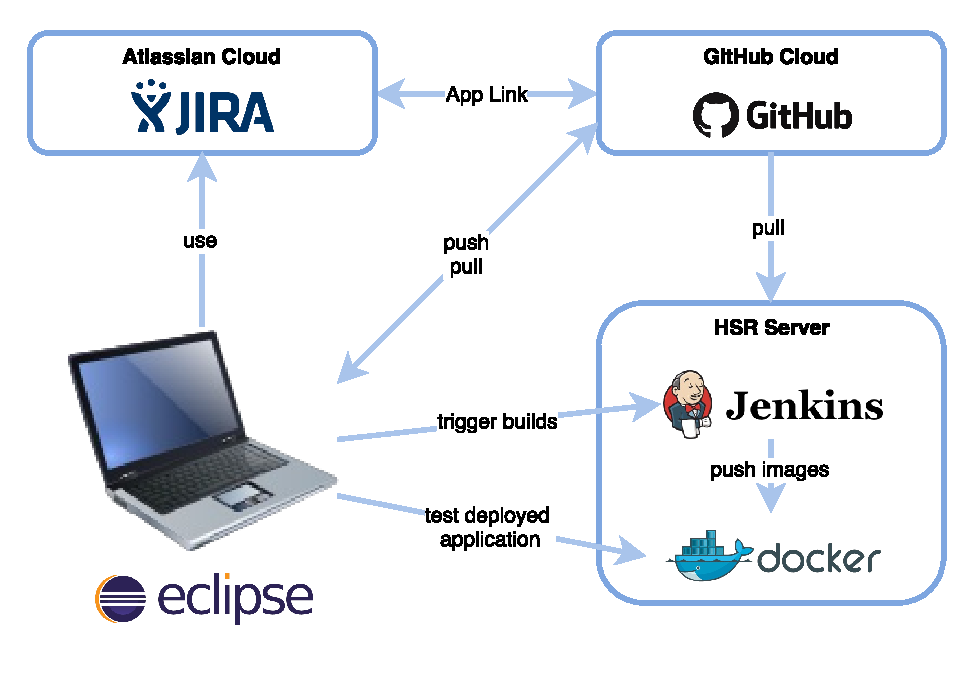
\includegraphics[scale=0.7]{diagrams/DevelopmentEnvironment.pdf}}
	\caption{Development Environment}
	\label{fig:devenvironment}
\end{figure}


\chapter{Meetings}

All minutes of meetings of the status meetings and workshops are listed in this Chapter.

\section{Workshop}

One workshop was organised refine the concept of coupling criteria.

\subsection{\formatdate{19}{10}{2015} at Z\"uhlke}

\textbf{Agenda}

\begin{enumerate}
\item Introduction
\item Brainstorming Coupling Criteria
\end{enumerate}

\textbf{Attendees}

\textbf{Notes}

\textbf{Decisions}

\textbf{Action Items}
\section{Feasibility Assessment}
\label{sec:feasibilityAssessment}

During sprint 2 we contacted Oliver Augenstein, professor of mathematics at \gls{HSR} for a feasibility assessment of the graph based approach. 

\subsection{\formatdate{13}{10}{2015} at HSR}

\textbf{Agenda}

\begin{enumerate}
\item Introduction and context
\item A weighted undirected graph approach
\item Alternative approaches or goals
\end{enumerate}

\textbf{Attendees:} Oliver Augenstein, Lukas Kölbener (KOE)

\textbf{General Feedback}

\begin{enumerate}
	\item The problem description and goal of the thesis might be too broad and ambitious. 
	\item An alternative approach to the problem could be to concentrate on coupling visualization instead of calculating candidate cuts. Data fields used more frequently by use cases could for example be colored with darker colors. A query language with queries like \enquote{show all transactions which operate on field X} would help to analyze a manually generated architecture. 
\end{enumerate}

\textbf{Notes on Graph Approach}

\begin{itemize}
	\item To develop a meaningful algorithm, we need a clear conception of the expected algorithm output for a given input.
	\item Normalizing the dimensions of every Coupling Criteria to one weight for each edge is challenging.  
	\item The Coupling Criteria characteristics are different. Modeling distance or clear constraints between vertices is difficult with weighted edges.
\end{itemize}

\textbf{Alternative Approaches}

\begin{itemize}
	\item To break down the problem into smaller pieces, every Coupling Criteria should be analyzed isolated of other Coupling Criteria. 
	\item A possible approach to achieve this is working with sets instead of a graph. For each Criteria a set of candidate cuts is calculated that meets all requirements of the Criteria. 
	\item Theoretically the number of candidate cuts is way too big to be calculated. Optimization is required.
	\item To analyze all Criteria, the algorithm tries to find a candidate cut existing in the solution set of every Criteria. 
\end{itemize}

\textbf{Conclusion}

We discussed these findings together and with our supervisor	. We decided to not change the focus to a more visualization based solution and still concentrate on finding optimal service cuts. The ideas for better visualization can still be integrated in the Service Cutter or used if early in the project it becomes clear that no sufficient algorithm can be found. 

The approach to assess precalculated candidate cuts per Coupling Criteria has many benefits over the graph based approach. It is more comprehensible as it is easier to debug or change and provides more information about the reasons why a candidate cut is a good solution for a system. Nevertheless, it first needs to be ascertained that the calculation can be done with a reasonable amount of time and resources. 
\section{Project Status}

Every sprint one or two status meetings where held to track the progress.

\subsection{Kick Off \formatdate{15}{9}{2015}}

\textbf{Time:} 14:00 – 15:15

\textbf{Next Meeting:} \formatdate{21}{9}{2015} 10:30

\textbf{Attendees:} Olaf Zimmermann (ZIO), Lukas Kölbener (KOE), Michael Gysel (GYS)

\textbf{Agenda}
\begin{itemize}
\item Meetings, Sprints
\item Aufgabenstellung
\item Discussion on the subject of the thesis
\end{itemize}

\textbf{Notes}
\begin{itemize}
\item The automatic REST interface of Apache ISIS could be an inspiration
\item Vaughn Vernon provides his DDD samples on \href{https://github.com/VaughnVernon/IDDD_Samples}{GitHub}
\item The provided article by Subbu Allamaraju is a must-read.
\item General approach: Start with business requirements (Use Cases, User Stories) and transform them into Components (e.g. UML). These Components are then modeled into services.
\item UML Components approach: Identification, Specification, Realization. (Our tool would probably support the step from spec to realization)
\item Possible quality attributes: Coupling, Cohesion, Security, Performance, Data volatility, Frequency of updates, Monitoring, Reconciliation, Consistency, Data invariants, Data Volumes
\item Structurizer by Simon Brown is a possible input format
\item C4: Context, Container, Components, Classes
\item Swagger is a possible output of the tool
\item Idea: Quality attributes should be specified on the level of fields instead of entities.
\item New item in the reading list: \url{https://msdn.microsoft.com/en-us/library/ms954587.aspx} 
\item NFR: Number of entities/fields to be supported
\end{itemize}

\textbf{Decisions}
\begin{itemize}
\item MoM and Meetings should be handled the same way as in the SA.
\item Project management should be < 10\% of the overall effort.
\item Model reconciliation is out of scope!
\end{itemize}

\textbf{Tasks}
\begin{itemize}
\item GYS: Send invite for the next meeting
\item GYS/KOE: Suggest dates for the intermediate presentation (end Oct, beginning of Nov)
\item ZIO: Send Aufgabenstellung via mail to GYS/KOE
\item ZIO: Bring UML Components book to the next meeting
\item ZIO: Book a room for the next meeting (21.9. 16:30)
\end{itemize}

\subsection{Status Meeting \formatdate{21}{9}{2015}}

\textbf{Time:} 10:30 – 12:00
 
\textbf{Next Meeting:} \formatdate{19}{10}{2015} 14:00-16:00 (Zühlke Office)
 
\textbf{Attendees:} Olaf Zimmermann (ZIO), Lukas Kölbener (KOE), Michael Gysel (GYS), Wolfgang Giersche
 
\textbf{Agenda}
\begin{itemize}
\item Scope and content of the thesis 
\item Project Organization / Review Meetings
\item Intellectual property rights
\end{itemize}

\textbf{Notes}
\begin{itemize}
\item Coupling Criterion / architectural significant requirements
\subitem Data confidentiality
\subitem SPI, Sensitive Personal Information
\subitem Structural volatility
\item Critique on automated scoring systems for IT architecture:
\subitem Pseudo accuracy, for example when mapping non functional requirements
\subitem Only one of many relevant criteria considered
\subitem => Make a sensitivity analysis to analyze the impact of weight-parameters
\item Define exactly what is meant with entity, bounded context and aggregates are within the system
\item Check Spark framework for algorithms
\item Check triple graph grammar for model transformations
\item Possible modes of system: Suggested bounded contexts are local (Modules, Components) or separated by network (Remote/ Microservices)
\item The data used in multiple bounded contexts should be part of the \enquote{published language} (DDD)
\item Dr. Gerald Reif will take the role of the expert
\end{itemize}

\textbf{Decisions}
\begin{itemize}
\item The target audience (Persona) are architects which use the system as assistance in taking architectural decisions
\item The produced results will be published on Github under the Apache 2.0 license
\item Meetings 
\subitem 19.10.2015, 14:00-16:00 Office Zühlke 
\subitem 22.10.2015, 09:00-10:00 HSR
\subitem 19.10.2015, 11:00-12:00 HSR
\end{itemize}

\textbf{Tasks}
\begin{itemize}
\item GYS/KOE: Review \enquote{Aufgabenstellung} and send back to ZIO
\item GYS/KOE: Send invitation for meetings
\item GYS/KOE: Authorize ZIO on Github repositories
\item Giersche: Find example project(s) with good complexity level and documentation (domain model, user stories, NFRs...). Clarify if the project can be published as an example within the thesis.
\end{itemize}

\subsection{Status Meeting \formatdate{15}{10}{2015}}

\textbf{Time:} 11:00 - 12:00

\textbf{Next Meetings:} \formatdate{19}{10}{2015} 14:00, Z\"uhlke; \formatdate{22}{10}{2015} 09:00, HSR
 
\textbf{Attendees:} Olaf Zimmermann (ZIO), Lukas Kölbener (KOE), Michael Gysel (GYS)

\textbf{Agenda}

\begin{itemize}
\item Thesis \& documentation progress
\item Outcome discussion with O. Augenstein // Complexity, alternative approaches
\item Date of intermediate presentation (Zwischenpr\"asentation)
\item Interest of industry contacts
\item Idea workshop Monday @ Z\"uhlke
\end{itemize}


\textbf{Notes}
\begin{itemize}
\item The thesis title needs to be finalized by mid November.
\item \enquote{Service} is a good candidate for the things produced by the service cutter. Conflicting definitions exist for \enquote{Service} of which some focus on business capability and others on providing a remote API. 
\item Possible example project candidates are Netstal (\url{http://wwww.netstal.com}) and the master thesis by Jonas Biedermann.
\item The clustering approach has multiple flaws which are hard to overcome. A new approach using theory of sets is inspired by the discussion with Prof. O. Augenstein and will be analyzed within this sprint. 
\item Good visualization of the service cutter input and good traceability within the tool might support the taking and documentation of architectural decisions.
\item Andreas Rinkel will take the role of the \enquote{Gegenleser} for this bachelor thesis.
\item ZIO provided further ideas and research material on the topic of coupling criteria and decomposition. 
\end{itemize}
 
\textbf{Tasks}
\begin{itemize}
\item ZIO: Send draft for legal rights agreement (15.10)
\item ALL: Sign legal rights agreement (19.10)
\item GYS/KOE: Return "UML Components" book to ZIO by next week (22.10)
\item ZIO: Find date for intermediate presentation during 9-11. November (21.10)
\end{itemize}


\subsection{Status Meeting \formatdate{22}{10}{2015}}
\label{sec:status22102015}

\textbf{Attendees}: Wolfgang Giersche, Olaf Zimmermann (ZIO), Lukas Kölbener (KOE), Michael Gysel (GYS)
 
\textbf{Next Meeting}: 19.11.2015, 11:00 @HSR / Skype

\textbf{Agenda}

\begin{itemize}
\item Admin: Sign paper regarding usage rights
\item Demo: Prototype, development environment
\item Coupling Criteria Catalog
\item Algorithms and coupling quantification
\item Sample project (not discussed)
\end{itemize}
 
\textbf{Notes}

\begin{itemize}
\item Maintainability is important. Coupling Criteria should be changeable with an appropriate effort.
\item Findings discussion on the algorithm / approach.
\subitem Calculating a score of every possible service cut is not possible.
\subitem New term: Candidate Service Cut.
\subitem Idea W.G.: Start with a heuristic approach like “Substantiv-Clustering”, a set of Candidate Service Cuts derived from a graph cluster or an analysis using only one Coupling Criteria.
\subitem Document needs to explain why we did not “just use a graph cluster”.
\item Three step approach is probably required
\subitem Determine a set of Candidate Service Cuts (perform once) (needs to be a smart solution – not a brute force approach! E.g. 100 possibilities.)
\subitem Assess all Candidates with a given set of weights to come up with a score.
\subitem Evaluate all Candidates with priorities by CC to find best choices.
\item Idea: Shake solution to improve it.
\end{itemize}
 
\textbf{Decisions}

\begin{itemize}
\item It is not an exact science – a good solution is enough.
\item No complete freeze of the CC catalog as of now.
\item Performance for 100 Entities, 2000 Fields:
\subitem Calculate Candidate Service Cuts (Steps 1\&2) – less than 10 minutes
\subitem Evaluate Candidates with parametrized weights (Step 3) – less than 5 seconds
\end{itemize}
 
\textbf{Action Items}

\begin{itemize}
\item GYS/KOE: Send documentation to ZIO for a review by the end of Oct.
\item GYS/KOE: Enhance Coupling Catalog with Decomposition Impact, Example (maybe from trading system), Measurement/Quantification, Type (Distance/Proximity/Constraint)
\end{itemize}

\subsection{HSR Status Meeting \formatdate{11}{11}{2015}}

\textbf{Attendees}: Olaf Zimmermann (ZIO), Lukas Kölbener (KOE), Michael Gysel (GYS)
 
\textbf{Next Meeting}: tbd

\textbf{Agenda}

\begin{itemize}
\item Status of thesis / development
\item Sprint Goals 3 \& 4
\item Sample Project
\item Personas
\item Final presentation
\item Discussion Thesis Review
\end{itemize}

\textbf{Notes}

\begin{itemize}
\item The cargo tracking sample application is currently being reimplemented. Maybe take a look at it to use it as test project.
\item Can we apply the service cutter to the service cutter domain model? Good for credibility to test one's own systems. 
\item Personas are very good. Add an Enterprise Architect.
\item Papers on coupling: (focus on object oriented code, not architecture!)
	\begin{itemize}
		\item \url{http://ieeexplore.ieee.org/stamp/stamp.jsp?tp=\&arnumber=1605186}
		\item \url{http://ieeexplore.ieee.org/stamp/stamp.jsp?tp=\&arnumber=4021375\&tag=1}
	\end{itemize}
\item Ideas for a renaming of \enquote{data field}:
	\begin{itemize}
		\item Micro entity
		\item Nano entity
		\item Candidate Entity
		\item Nano service
	\end{itemize}
\item Describe every concept with an example
\end{itemize}

\textbf{Additional feedback by ZIO}
\begin{itemize}
\item Explain that criteria catalog does not aim for completeness.
\item Introduce example earlier .
\item Visualize coupling types.
\item Apply Service Cutter concepts/tool to Service Cutter design (as an additional validation step in last sprint).
\item Generalize from use case/user story as input (of busienss-level operations) to conceptual components (e.g. CRC cards)?
\item Make sure that all tool output can be reproduced, or that tool output can be consumed as input (e.g. in follow on projects or subsequent but delayed iterations in a project), consider previously proposed service cuts as one special type of legacy system constraint?
\end{itemize}

\textbf{Decisions}

\begin{itemize}
\item Notation
	\begin{itemize}
	\item Web uppercase
	\item service lowercase
	\item coupling criteria lowercase
	\item Service Cutter uppercase
	\end{itemize}
\item Final term instead of \enquote{data field} should be finalized in the next meeting.
\end{itemize}
 
\textbf{Action Items}

\begin{itemize}
\item ZIO: Find date for Abschlusspräsentation. (14. – 22. Januar)
\item ZIO: Send mentioned papers/books on pages 8 and 11.
\item GYS/KOE: Prepare suggestions for meetings in December.
\end{itemize}



\subsection{Status Meeting \formatdate{20}{11}{2015}}

\textbf{Attendees}: Wolfgang Giersche, Olaf Zimmermann (ZIO), Lukas Kölbener (KOE), Michael Gysel (GYS)
 
\textbf{Next Meeting}: \formatdate{4}{12}{2015}, Zühlke, Schlieren

\textbf{Agenda}

\begin{itemize}
\item Evaluation of Algorithms
\item Overview of Coupling Criteria Types and Scoring
\item Demo \enquote{Trading System}
\item Scope of Sprint 4
\item Various items
\end{itemize}

\textbf{Decisions}
 
Priority for the next sprint are:
\begin{itemize}
\item DDD Sample
\item Polishing of UI, small enhancements. See \enquote{Notes ZIO}.
\end{itemize}

\textbf{Notes ZIO}
\begin{itemize}
\item Define/explain and possibly challenge/refine all new names/concepts, expsecially those exposed in UI, e.g. \enquote{Variant}, \enquote{Field Group}, \dots
\item If input is a set of nano entities (new name of data field, which is ok with me), what is the output? Services? Microservices? Entitites? Bounded contexts? Current UI says \enquote{Service A}, \enquote{Service B} etc. (which is ok, but input/output terminology should be consistent and symmetric) 
\item Feature requests/ideas incl. UI enhancements:

	\begin{itemize}
	\item Save output (service cuts suggested by alg.) in a machine-processable form, JSON at a minmum (so that next tool in chain can pick them up); ideally, this output takes the form of serialized CRC cards and/or Swagger definitions 
	\item Ability to store and reload all settings done by user, e.g. prioritizations
	\item Stepwise forward/backward button, or before/after feature to support incrementa design and what-if analyses (as a service modeler, I want to see how service cut changes when I update one setting at a time, and I also want to be able to undo my last changes)
	\item Show output of several algorithms in parallel/in comparison (workaround/simpleo solution: two browser tabs wordking with same model in backend)
	\item \enquote{Reset to default settings} button (e.g. for prioritizations)
	\item Graph metrics (analysis) with simple aggregation gree-yellow-red \enquote{how good is the current service cut} (according to some rules of thumb from OOAD or SOA design methods; I  can provide some input in next meeting)
	\item Make defaults and score values [-10…10] configurable (e.g. in config file or system property)
	\item Ability to define own variants (with weight scores), e.g. what if I want to specific a security classification \enquote{very critical} in addition to those shown in demo
	\end{itemize}

\end{itemize}

\textbf{General Notes}

\begin{itemize}
\item Coupling types visualization:

	\begin{itemize}
	\item Order of rows: Domain, Quality, Infrastructure, Security
	\item Empty boxes: Explain! (List is not exhaustive – but other types were not part of the outcome of the workshop)
	\item Cohesion instead of Cohesiveness? (Cohesion already has a meaning)
	\item Goal: only one term in the final version
	\end{itemize}

\item Scoring

	\begin{itemize}
		\item -10 to 10 is a good range for human beings. Technically -1 to 1 would be at least as good.
		\item Explain reasons why Fibonacci numbers were selected for the priorities. (Quote similar paper where Fibonacci were used for priorities or perform an A/B testing.)
		\item Document sample with a few priorities and a second example with all/high priorities used.
		\item Thoroughly document justify the scoring process.
		\item The weights are opinions. Make configurable and document. 
		\item Introduce all introduced terms such as variants, field groups, score, weight.
		\item Find better term than “variant”.
		\item Discussion: Data volumes, document why it should scale. Do tests.
		\item Document defaults and make them configurable.
	\end{itemize}

\item Document the import and how it works in detail. Add defaults to CC cards?
\item Document the trading example tests.
\item Are CRC card similar to our output?
\item \enquote{Parameters} instead of \enquote{Params}
\item Document the different Algorithms.
\item Document the value of the Service Cutter to an architect! Present some unexpected but good decompositions. Also educational aspects.
\item Document the value of the Service Cutter in the process of going from a monolith to a service oriented architecture. 
\item Add some kind of hint on whether the suggested cuts are good or not (traffic lights).
\item Source code: Should not be embarrassing but does not have to be perfect. It still is a prototype.
\item The tool should produce some kind of output.

\end{itemize}

\subsection{Status Meeting \formatdate{4}{12}{2015}}

\textbf{Attendees}: Wolfgang Giersche, Olaf Zimmermann (ZIO), Lukas Kölbener (KOE), Michael Gysel (GYS)

\textbf{Agenda} 

\begin{itemize}
\item Progress Update
\item DDD Sample “Cargo Tracking” Analysis 
\item Outlook: last week
\end{itemize}

\textbf{Decisions}

\begin{itemize}
\item It is sufficient that not all described coupling criteria are implemented within the Service Cutter. The main goal of the thesis is the proof of concept and not completeness.
\item Priorities:
	\begin{itemize}
	\item Wolfgang Giersche: Additional Leung layer and analysis Leung vs. Girvan-Newman.
	\item ZIO: Being able to work with Service Cutter, change settings, store results and use results for further processing in a toolkit chain. Being able to give the tool to another person to work with.
	\item Decision: Use the remaining time to wrap up Service Cutter functionality and usability with future work in mind. (Risk is too high and resources are too short.)
	\end{itemize}

\end{itemize}


\textbf{Action Items}

\begin{itemize}
\item ZIO: Send invitation for the final presentation to Wolfgang Giersche.
\item GYS/KOE: Send documentation and tool access for review to ZIO until 07.12.15 5pm.
\end{itemize}

\textbf{Notes }
\begin{itemize}
\item Document results of tests with expectation comparison. Define in a measurable way what a \enquote{good} or \enquote{bad} result is (test systems analysis).
\item Comparison Leung vs. Girvan-Newman: Different quality of output with exactly the same input. 
\item Document comparison with same number of services.
\item DDD Sample use cases have been reverse engineered from the sample source code.
\item Conduct a sensitivity analysis on priorities and weights.
\item Document evolutionary architecture, Fowler's \enquote{Monolith to Microservices}-approach with number of services as a parameter. 
\item Not defining number of services but receiving a suggestion by the Service Cutter has the advantage of avoiding to prejudice the solution.  
\item Document further analysis and integration of MCL in \enquote{Future Work} chapter.
\item Additional Layer for Leung in \enquote{Future Work} chapter $\rightarrow$ Machine Learning?
\item Document which criteria have been defined in the workshop and which were added later.  
\item Document \enquote{Communication} Criteria separately as \enquote{Candidate Criteria} to be implemented in \enquote{Future Work}.
\end{itemize}

\section{Presentation}

\subsection{Intermediary Presentation \formatdate{11}{11}{2015}}

\textbf{Attendees:} Gerald Reif (ipt), Andreas Rinkel (HSR), Olaf Zimmermann (HSR), Lukas Kölbener, Michael Gysel

\textbf{Agenda}

\begin{itemize}
\item Introduction
\item Thesis
\item Approach
\item Demo
\item Next steps
\end{itemize}


\textbf{Notes}

\begin{itemize}
\item Clearly introduce the goal of the thesis / the tool.
	\begin{itemize}
	\item We aim to support the architect --– not replace him.
	\item We aim to decompose services --– not compose them.
	\item Our goal is to build good services. Composing them into applications, defining technology or the communication between services is out of scope.
	\end{itemize}
\item Answer question: What is the tool going to do for me?
\item Phrase: \enquote{Modell- oder Eventgetrieben}. Where do we stand?
\item Properly introduce the term service in the thesis. Also relate to operations and business logic.
\item Define entity. (Not the db term! Relate to the DDD entity. Also includes logic – not just data.)
\item Answer question: Why do I need services at all?
\item Introduce the handling of operations early in documentation.
\item How are future iterations reflected? Can we feed the service cut output back into the system for the next iteration? (Feature Request!)
\item Document how the coupling criteria catalog was developed.
\item Document the comprehensiveness of the cc catalog.
\item Possible real world problem: Too much data is required. Where do we get it from, how to we enter it? Provide good defaults!
\item Create images/icons for types of coupling criteria.
\end{itemize}


\textbf{Presentation}

\begin{itemize}
\item Introduce target group (architect, developer, designer) earlier.
\item Flip software layers diagram vertically.
\item Spell out abbreviations.
\item Introduce cited persons.
\end{itemize}

%\section{Project Management Methodology}

We chose Scrum as the project management methodology for this bachelor thesis. Scrum specifies an iterative and incremental approach which encourages a high involvement of the customer. This characteristics suit the requirements of a bachelor thesis well,
as it provides only a short project definition at project start and, in our case, requires close collaboration with our advisor and industry partner.

%\clearpage
\section{Project Roles}

Scrum defines three project roles — the product owner, the scrum master and the development
team. As this bachelor thesis is an academical project, the scrum roles could
not be mapped one to one. This Section introduces the involved persons and their roles
in the project.

\subsection{HSR Supervisor}

\begin{minipage}[t]{0.25\textwidth}
	\vspace{0pt}
	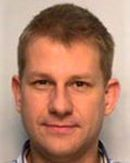
\includegraphics[width=0.8\textwidth]{olz.jpg}
\end{minipage}
\begin{minipage}[t]{0.8\textwidth}
	\vspace{10pt}
	Prof. Dr. Olaf Zimmermann is the \gls{HSR} supervisor of this thesis and incorporates both, the role of the product owner and scrum master. \textit{Product} in this context refers to the thesis itself as well as the functional product. He ensures that all requirements by HSR for a bachelor thesis are met and decides in last instance about the scope of the thesis. 
	As supervisor and coach of the development team, Mr. Zimmermann also performs part of the scrum master role as he coaches the development team.
\end{minipage}


\subsection{Industry Partner}

Our industry partner Zühlke Engineering, represented by W. Giersche, ensured the functional relevancy of this thesis. Mr. Giersche contributed valuable experience from many software engineering projects. He represented part of the product owner role as he played an important role in the functional prioritization to maximize the business value. Being an experienced software architect, he also contributed to the coupling criteria catalog by conducting workshops.


\subsection{Project Team}

Michael Gysel and Lukas Kölbener formed the development team. They worked as an interdisciplinary team in which both were responsible for each part of the project. Both being Certified ScrumMasters\textregistered\cite{scrummaster}, they incorporated part of the scrum master role as they helped maintaining the product backlog and organized everything for correct sprint operation.

\begin{minipage}[t]{0.25\textwidth}
	\vspace{0pt}
	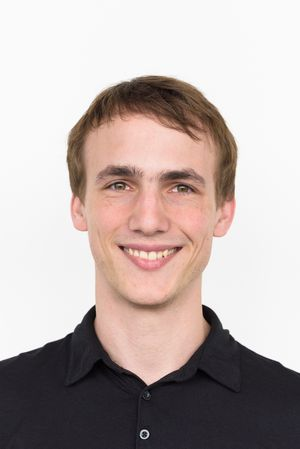
\includegraphics[width=0.8\textwidth]{lukas.jpg}
\end{minipage}
\begin{minipage}[t]{0.8\textwidth}
	\vspace{20pt}
	Lukas Kölbener is an information technology student at \gls{HSR} in his 9\textsuperscript{th} semester. He works part time as Java developer for Super Computing Systems AG in Zurich, building ticket vending machines for the public transport industry.
	\newline
\end{minipage}

\begin{minipage}[t]{0.25\textwidth}
	\vspace{0pt}
	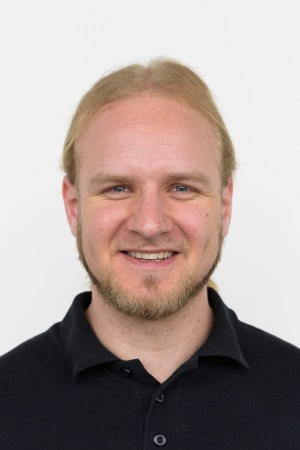
\includegraphics[width=0.8\textwidth]{michi.jpg}
\end{minipage}
\begin{minipage}[t]{0.8\textwidth}
	\vspace{20pt}
	Michael Gysel is an information technology student at \gls{HSR} in his 9\textsuperscript{th} semester. He works part time as Java Developer for FIS, a global provider for banking and payments technologies.
	\newline
\end{minipage}


%\include{anhang_d} % 
%\include{anhang_e} % 

%\renewcommand{\glossarypreamble}{Descriptions of Glossary items have mainly been taken from Wikipedia.org.\newline\newline}

\printglossaries


%%%----------------------------------------------------------
\MakeBibliography
%%%----------------------------------------------------------


\end{document}
